
% Default to the notebook output style

    


% Inherit from the specified cell style.




    
\documentclass[11pt]{article}

\usepackage {float}   
    
    
    \usepackage[T1]{fontenc}
    % Nicer default font (+ math font) than Computer Modern for most use cases
    \usepackage{mathpazo}

    % Basic figure setup, for now with no caption control since it's done
    % automatically by Pandoc (which extracts ![](path) syntax from Markdown).
    \usepackage{graphicx}
    % We will generate all images so they have a width \maxwidth. This means
    % that they will get their normal width if they fit onto the page, but
    % are scaled down if they would overflow the margins.
    \makeatletter
    \def\maxwidth{\ifdim\Gin@nat@width>\linewidth\linewidth
    \else\Gin@nat@width\fi}
    \makeatother
    \let\Oldincludegraphics\includegraphics
    % Set max figure width to be 80% of text width, for now hardcoded.
    \renewcommand{\includegraphics}[1]{\Oldincludegraphics[width=.8\maxwidth]{#1}}
    % Ensure that by default, figures have no caption (until we provide a
    % proper Figure object with a Caption API and a way to capture that
    % in the conversion process - todo).
    \usepackage{caption}
    \DeclareCaptionLabelFormat{nolabel}{}
    \captionsetup{labelformat=nolabel}

    \usepackage{adjustbox} % Used to constrain images to a maximum size 
    \usepackage{xcolor} % Allow colors to be defined
    \usepackage{enumerate} % Needed for markdown enumerations to work
    \usepackage{geometry} % Used to adjust the document margins
    \usepackage{amsmath} % Equations
    \usepackage{amssymb} % Equations
    \usepackage{textcomp} % defines textquotesingle
    % Hack from http://tex.stackexchange.com/a/47451/13684:
    \AtBeginDocument{%
        \def\PYZsq{\textquotesingle}% Upright quotes in Pygmentized code
    }
    \usepackage{upquote} % Upright quotes for verbatim code
    \usepackage{eurosym} % defines \euro
    \usepackage[mathletters]{ucs} % Extended unicode (utf-8) support
    \usepackage[utf8x]{inputenc} % Allow utf-8 characters in the tex document
    \usepackage{fancyvrb} % verbatim replacement that allows latex
    \usepackage{grffile} % extends the file name processing of package graphics 
                         % to support a larger range 
    % The hyperref package gives us a pdf with properly built
    % internal navigation ('pdf bookmarks' for the table of contents,
    % internal cross-reference links, web links for URLs, etc.)
    \usepackage{hyperref}
    \usepackage{longtable} % longtable support required by pandoc >1.10
    \usepackage{booktabs}  % table support for pandoc > 1.12.2
    \usepackage[inline]{enumitem} % IRkernel/repr support (it uses the enumerate* environment)
    \usepackage[normalem]{ulem} % ulem is needed to support strikethroughs (\sout)
                                % normalem makes italics be italics, not underlines
    \usepackage{mathrsfs}
    

    
    
    % Colors for the hyperref package
    \definecolor{urlcolor}{rgb}{0,.145,.698}
    \definecolor{linkcolor}{rgb}{.71,0.21,0.01}
    \definecolor{citecolor}{rgb}{.12,.54,.11}

    % ANSI colors
    \definecolor{ansi-black}{HTML}{3E424D}
    \definecolor{ansi-black-intense}{HTML}{282C36}
    \definecolor{ansi-red}{HTML}{E75C58}
    \definecolor{ansi-red-intense}{HTML}{B22B31}
    \definecolor{ansi-green}{HTML}{00A250}
    \definecolor{ansi-green-intense}{HTML}{007427}
    \definecolor{ansi-yellow}{HTML}{DDB62B}
    \definecolor{ansi-yellow-intense}{HTML}{B27D12}
    \definecolor{ansi-blue}{HTML}{208FFB}
    \definecolor{ansi-blue-intense}{HTML}{0065CA}
    \definecolor{ansi-magenta}{HTML}{D160C4}
    \definecolor{ansi-magenta-intense}{HTML}{A03196}
    \definecolor{ansi-cyan}{HTML}{60C6C8}
    \definecolor{ansi-cyan-intense}{HTML}{258F8F}
    \definecolor{ansi-white}{HTML}{C5C1B4}
    \definecolor{ansi-white-intense}{HTML}{A1A6B2}
    \definecolor{ansi-default-inverse-fg}{HTML}{FFFFFF}
    \definecolor{ansi-default-inverse-bg}{HTML}{000000}

    % commands and environments needed by pandoc snippets
    % extracted from the output of `pandoc -s`
    \providecommand{\tightlist}{%
      \setlength{\itemsep}{0pt}\setlength{\parskip}{0pt}}
    \DefineVerbatimEnvironment{Highlighting}{Verbatim}{commandchars=\\\{\}}
    % Add ',fontsize=\small' for more characters per line
    \newenvironment{Shaded}{}{}
    \newcommand{\KeywordTok}[1]{\textcolor[rgb]{0.00,0.44,0.13}{\textbf{{#1}}}}
    \newcommand{\DataTypeTok}[1]{\textcolor[rgb]{0.56,0.13,0.00}{{#1}}}
    \newcommand{\DecValTok}[1]{\textcolor[rgb]{0.25,0.63,0.44}{{#1}}}
    \newcommand{\BaseNTok}[1]{\textcolor[rgb]{0.25,0.63,0.44}{{#1}}}
    \newcommand{\FloatTok}[1]{\textcolor[rgb]{0.25,0.63,0.44}{{#1}}}
    \newcommand{\CharTok}[1]{\textcolor[rgb]{0.25,0.44,0.63}{{#1}}}
    \newcommand{\StringTok}[1]{\textcolor[rgb]{0.25,0.44,0.63}{{#1}}}
    \newcommand{\CommentTok}[1]{\textcolor[rgb]{0.38,0.63,0.69}{\textit{{#1}}}}
    \newcommand{\OtherTok}[1]{\textcolor[rgb]{0.00,0.44,0.13}{{#1}}}
    \newcommand{\AlertTok}[1]{\textcolor[rgb]{1.00,0.00,0.00}{\textbf{{#1}}}}
    \newcommand{\FunctionTok}[1]{\textcolor[rgb]{0.02,0.16,0.49}{{#1}}}
    \newcommand{\RegionMarkerTok}[1]{{#1}}
    \newcommand{\ErrorTok}[1]{\textcolor[rgb]{1.00,0.00,0.00}{\textbf{{#1}}}}
    \newcommand{\NormalTok}[1]{{#1}}
    
    % Additional commands for more recent versions of Pandoc
    \newcommand{\ConstantTok}[1]{\textcolor[rgb]{0.53,0.00,0.00}{{#1}}}
    \newcommand{\SpecialCharTok}[1]{\textcolor[rgb]{0.25,0.44,0.63}{{#1}}}
    \newcommand{\VerbatimStringTok}[1]{\textcolor[rgb]{0.25,0.44,0.63}{{#1}}}
    \newcommand{\SpecialStringTok}[1]{\textcolor[rgb]{0.73,0.40,0.53}{{#1}}}
    \newcommand{\ImportTok}[1]{{#1}}
    \newcommand{\DocumentationTok}[1]{\textcolor[rgb]{0.73,0.13,0.13}{\textit{{#1}}}}
    \newcommand{\AnnotationTok}[1]{\textcolor[rgb]{0.38,0.63,0.69}{\textbf{\textit{{#1}}}}}
    \newcommand{\CommentVarTok}[1]{\textcolor[rgb]{0.38,0.63,0.69}{\textbf{\textit{{#1}}}}}
    \newcommand{\VariableTok}[1]{\textcolor[rgb]{0.10,0.09,0.49}{{#1}}}
    \newcommand{\ControlFlowTok}[1]{\textcolor[rgb]{0.00,0.44,0.13}{\textbf{{#1}}}}
    \newcommand{\OperatorTok}[1]{\textcolor[rgb]{0.40,0.40,0.40}{{#1}}}
    \newcommand{\BuiltInTok}[1]{{#1}}
    \newcommand{\ExtensionTok}[1]{{#1}}
    \newcommand{\PreprocessorTok}[1]{\textcolor[rgb]{0.74,0.48,0.00}{{#1}}}
    \newcommand{\AttributeTok}[1]{\textcolor[rgb]{0.49,0.56,0.16}{{#1}}}
    \newcommand{\InformationTok}[1]{\textcolor[rgb]{0.38,0.63,0.69}{\textbf{\textit{{#1}}}}}
    \newcommand{\WarningTok}[1]{\textcolor[rgb]{0.38,0.63,0.69}{\textbf{\textit{{#1}}}}}
    
    
    % Define a nice break command that doesn't care if a line doesn't already
    % exist.
    \def\br{\hspace*{\fill} \\* }
    % Math Jax compatibility definitions
    \def\gt{>}
    \def\lt{<}
    \let\Oldtex\TeX
    \let\Oldlatex\LaTeX
    \renewcommand{\TeX}{\textrm{\Oldtex}}
    \renewcommand{\LaTeX}{\textrm{\Oldlatex}}
    % Document parameters
    % Document title
    \title{Bitcoin Price Prediction using LSTM and ARIMA with Quandl API}
    
    
    
    
    

    % Pygments definitions
    
\makeatletter
\def\PY@reset{\let\PY@it=\relax \let\PY@bf=\relax%
    \let\PY@ul=\relax \let\PY@tc=\relax%
    \let\PY@bc=\relax \let\PY@ff=\relax}
\def\PY@tok#1{\csname PY@tok@#1\endcsname}
\def\PY@toks#1+{\ifx\relax#1\empty\else%
    \PY@tok{#1}\expandafter\PY@toks\fi}
\def\PY@do#1{\PY@bc{\PY@tc{\PY@ul{%
    \PY@it{\PY@bf{\PY@ff{#1}}}}}}}
\def\PY#1#2{\PY@reset\PY@toks#1+\relax+\PY@do{#2}}

\expandafter\def\csname PY@tok@w\endcsname{\def\PY@tc##1{\textcolor[rgb]{0.73,0.73,0.73}{##1}}}
\expandafter\def\csname PY@tok@c\endcsname{\let\PY@it=\textit\def\PY@tc##1{\textcolor[rgb]{0.25,0.50,0.50}{##1}}}
\expandafter\def\csname PY@tok@cp\endcsname{\def\PY@tc##1{\textcolor[rgb]{0.74,0.48,0.00}{##1}}}
\expandafter\def\csname PY@tok@k\endcsname{\let\PY@bf=\textbf\def\PY@tc##1{\textcolor[rgb]{0.00,0.50,0.00}{##1}}}
\expandafter\def\csname PY@tok@kp\endcsname{\def\PY@tc##1{\textcolor[rgb]{0.00,0.50,0.00}{##1}}}
\expandafter\def\csname PY@tok@kt\endcsname{\def\PY@tc##1{\textcolor[rgb]{0.69,0.00,0.25}{##1}}}
\expandafter\def\csname PY@tok@o\endcsname{\def\PY@tc##1{\textcolor[rgb]{0.40,0.40,0.40}{##1}}}
\expandafter\def\csname PY@tok@ow\endcsname{\let\PY@bf=\textbf\def\PY@tc##1{\textcolor[rgb]{0.67,0.13,1.00}{##1}}}
\expandafter\def\csname PY@tok@nb\endcsname{\def\PY@tc##1{\textcolor[rgb]{0.00,0.50,0.00}{##1}}}
\expandafter\def\csname PY@tok@nf\endcsname{\def\PY@tc##1{\textcolor[rgb]{0.00,0.00,1.00}{##1}}}
\expandafter\def\csname PY@tok@nc\endcsname{\let\PY@bf=\textbf\def\PY@tc##1{\textcolor[rgb]{0.00,0.00,1.00}{##1}}}
\expandafter\def\csname PY@tok@nn\endcsname{\let\PY@bf=\textbf\def\PY@tc##1{\textcolor[rgb]{0.00,0.00,1.00}{##1}}}
\expandafter\def\csname PY@tok@ne\endcsname{\let\PY@bf=\textbf\def\PY@tc##1{\textcolor[rgb]{0.82,0.25,0.23}{##1}}}
\expandafter\def\csname PY@tok@nv\endcsname{\def\PY@tc##1{\textcolor[rgb]{0.10,0.09,0.49}{##1}}}
\expandafter\def\csname PY@tok@no\endcsname{\def\PY@tc##1{\textcolor[rgb]{0.53,0.00,0.00}{##1}}}
\expandafter\def\csname PY@tok@nl\endcsname{\def\PY@tc##1{\textcolor[rgb]{0.63,0.63,0.00}{##1}}}
\expandafter\def\csname PY@tok@ni\endcsname{\let\PY@bf=\textbf\def\PY@tc##1{\textcolor[rgb]{0.60,0.60,0.60}{##1}}}
\expandafter\def\csname PY@tok@na\endcsname{\def\PY@tc##1{\textcolor[rgb]{0.49,0.56,0.16}{##1}}}
\expandafter\def\csname PY@tok@nt\endcsname{\let\PY@bf=\textbf\def\PY@tc##1{\textcolor[rgb]{0.00,0.50,0.00}{##1}}}
\expandafter\def\csname PY@tok@nd\endcsname{\def\PY@tc##1{\textcolor[rgb]{0.67,0.13,1.00}{##1}}}
\expandafter\def\csname PY@tok@s\endcsname{\def\PY@tc##1{\textcolor[rgb]{0.73,0.13,0.13}{##1}}}
\expandafter\def\csname PY@tok@sd\endcsname{\let\PY@it=\textit\def\PY@tc##1{\textcolor[rgb]{0.73,0.13,0.13}{##1}}}
\expandafter\def\csname PY@tok@si\endcsname{\let\PY@bf=\textbf\def\PY@tc##1{\textcolor[rgb]{0.73,0.40,0.53}{##1}}}
\expandafter\def\csname PY@tok@se\endcsname{\let\PY@bf=\textbf\def\PY@tc##1{\textcolor[rgb]{0.73,0.40,0.13}{##1}}}
\expandafter\def\csname PY@tok@sr\endcsname{\def\PY@tc##1{\textcolor[rgb]{0.73,0.40,0.53}{##1}}}
\expandafter\def\csname PY@tok@ss\endcsname{\def\PY@tc##1{\textcolor[rgb]{0.10,0.09,0.49}{##1}}}
\expandafter\def\csname PY@tok@sx\endcsname{\def\PY@tc##1{\textcolor[rgb]{0.00,0.50,0.00}{##1}}}
\expandafter\def\csname PY@tok@m\endcsname{\def\PY@tc##1{\textcolor[rgb]{0.40,0.40,0.40}{##1}}}
\expandafter\def\csname PY@tok@gh\endcsname{\let\PY@bf=\textbf\def\PY@tc##1{\textcolor[rgb]{0.00,0.00,0.50}{##1}}}
\expandafter\def\csname PY@tok@gu\endcsname{\let\PY@bf=\textbf\def\PY@tc##1{\textcolor[rgb]{0.50,0.00,0.50}{##1}}}
\expandafter\def\csname PY@tok@gd\endcsname{\def\PY@tc##1{\textcolor[rgb]{0.63,0.00,0.00}{##1}}}
\expandafter\def\csname PY@tok@gi\endcsname{\def\PY@tc##1{\textcolor[rgb]{0.00,0.63,0.00}{##1}}}
\expandafter\def\csname PY@tok@gr\endcsname{\def\PY@tc##1{\textcolor[rgb]{1.00,0.00,0.00}{##1}}}
\expandafter\def\csname PY@tok@ge\endcsname{\let\PY@it=\textit}
\expandafter\def\csname PY@tok@gs\endcsname{\let\PY@bf=\textbf}
\expandafter\def\csname PY@tok@gp\endcsname{\let\PY@bf=\textbf\def\PY@tc##1{\textcolor[rgb]{0.00,0.00,0.50}{##1}}}
\expandafter\def\csname PY@tok@go\endcsname{\def\PY@tc##1{\textcolor[rgb]{0.53,0.53,0.53}{##1}}}
\expandafter\def\csname PY@tok@gt\endcsname{\def\PY@tc##1{\textcolor[rgb]{0.00,0.27,0.87}{##1}}}
\expandafter\def\csname PY@tok@err\endcsname{\def\PY@bc##1{\setlength{\fboxsep}{0pt}\fcolorbox[rgb]{1.00,0.00,0.00}{1,1,1}{\strut ##1}}}
\expandafter\def\csname PY@tok@kc\endcsname{\let\PY@bf=\textbf\def\PY@tc##1{\textcolor[rgb]{0.00,0.50,0.00}{##1}}}
\expandafter\def\csname PY@tok@kd\endcsname{\let\PY@bf=\textbf\def\PY@tc##1{\textcolor[rgb]{0.00,0.50,0.00}{##1}}}
\expandafter\def\csname PY@tok@kn\endcsname{\let\PY@bf=\textbf\def\PY@tc##1{\textcolor[rgb]{0.00,0.50,0.00}{##1}}}
\expandafter\def\csname PY@tok@kr\endcsname{\let\PY@bf=\textbf\def\PY@tc##1{\textcolor[rgb]{0.00,0.50,0.00}{##1}}}
\expandafter\def\csname PY@tok@bp\endcsname{\def\PY@tc##1{\textcolor[rgb]{0.00,0.50,0.00}{##1}}}
\expandafter\def\csname PY@tok@fm\endcsname{\def\PY@tc##1{\textcolor[rgb]{0.00,0.00,1.00}{##1}}}
\expandafter\def\csname PY@tok@vc\endcsname{\def\PY@tc##1{\textcolor[rgb]{0.10,0.09,0.49}{##1}}}
\expandafter\def\csname PY@tok@vg\endcsname{\def\PY@tc##1{\textcolor[rgb]{0.10,0.09,0.49}{##1}}}
\expandafter\def\csname PY@tok@vi\endcsname{\def\PY@tc##1{\textcolor[rgb]{0.10,0.09,0.49}{##1}}}
\expandafter\def\csname PY@tok@vm\endcsname{\def\PY@tc##1{\textcolor[rgb]{0.10,0.09,0.49}{##1}}}
\expandafter\def\csname PY@tok@sa\endcsname{\def\PY@tc##1{\textcolor[rgb]{0.73,0.13,0.13}{##1}}}
\expandafter\def\csname PY@tok@sb\endcsname{\def\PY@tc##1{\textcolor[rgb]{0.73,0.13,0.13}{##1}}}
\expandafter\def\csname PY@tok@sc\endcsname{\def\PY@tc##1{\textcolor[rgb]{0.73,0.13,0.13}{##1}}}
\expandafter\def\csname PY@tok@dl\endcsname{\def\PY@tc##1{\textcolor[rgb]{0.73,0.13,0.13}{##1}}}
\expandafter\def\csname PY@tok@s2\endcsname{\def\PY@tc##1{\textcolor[rgb]{0.73,0.13,0.13}{##1}}}
\expandafter\def\csname PY@tok@sh\endcsname{\def\PY@tc##1{\textcolor[rgb]{0.73,0.13,0.13}{##1}}}
\expandafter\def\csname PY@tok@s1\endcsname{\def\PY@tc##1{\textcolor[rgb]{0.73,0.13,0.13}{##1}}}
\expandafter\def\csname PY@tok@mb\endcsname{\def\PY@tc##1{\textcolor[rgb]{0.40,0.40,0.40}{##1}}}
\expandafter\def\csname PY@tok@mf\endcsname{\def\PY@tc##1{\textcolor[rgb]{0.40,0.40,0.40}{##1}}}
\expandafter\def\csname PY@tok@mh\endcsname{\def\PY@tc##1{\textcolor[rgb]{0.40,0.40,0.40}{##1}}}
\expandafter\def\csname PY@tok@mi\endcsname{\def\PY@tc##1{\textcolor[rgb]{0.40,0.40,0.40}{##1}}}
\expandafter\def\csname PY@tok@il\endcsname{\def\PY@tc##1{\textcolor[rgb]{0.40,0.40,0.40}{##1}}}
\expandafter\def\csname PY@tok@mo\endcsname{\def\PY@tc##1{\textcolor[rgb]{0.40,0.40,0.40}{##1}}}
\expandafter\def\csname PY@tok@ch\endcsname{\let\PY@it=\textit\def\PY@tc##1{\textcolor[rgb]{0.25,0.50,0.50}{##1}}}
\expandafter\def\csname PY@tok@cm\endcsname{\let\PY@it=\textit\def\PY@tc##1{\textcolor[rgb]{0.25,0.50,0.50}{##1}}}
\expandafter\def\csname PY@tok@cpf\endcsname{\let\PY@it=\textit\def\PY@tc##1{\textcolor[rgb]{0.25,0.50,0.50}{##1}}}
\expandafter\def\csname PY@tok@c1\endcsname{\let\PY@it=\textit\def\PY@tc##1{\textcolor[rgb]{0.25,0.50,0.50}{##1}}}
\expandafter\def\csname PY@tok@cs\endcsname{\let\PY@it=\textit\def\PY@tc##1{\textcolor[rgb]{0.25,0.50,0.50}{##1}}}

\def\PYZbs{\char`\\}
\def\PYZus{\char`\_}
\def\PYZob{\char`\{}
\def\PYZcb{\char`\}}
\def\PYZca{\char`\^}
\def\PYZam{\char`\&}
\def\PYZlt{\char`\<}
\def\PYZgt{\char`\>}
\def\PYZsh{\char`\#}
\def\PYZpc{\char`\%}
\def\PYZdl{\char`\$}
\def\PYZhy{\char`\-}
\def\PYZsq{\char`\'}
\def\PYZdq{\char`\"}
\def\PYZti{\char`\~}
% for compatibility with earlier versions
\def\PYZat{@}
\def\PYZlb{[}
\def\PYZrb{]}
\makeatother


    % Exact colors from NB
    \definecolor{incolor}{rgb}{0.0, 0.0, 0.5}
    \definecolor{outcolor}{rgb}{0.545, 0.0, 0.0}



    
    % Prevent overflowing lines due to hard-to-break entities
    \sloppy 
    % Setup hyperref package
    \hypersetup{
      breaklinks=true,  % so long urls are correctly broken across lines
      colorlinks=true,
      urlcolor=urlcolor,
      linkcolor=linkcolor,
      citecolor=citecolor,
      }
    % Slightly bigger margins than the latex defaults
    
    \geometry{verbose,tmargin=1in,bmargin=1in,lmargin=1in,rmargin=1in}
    
    

    \begin{document}
    
    
    \maketitle
    
    

    
    \hypertarget{introduction}{%
\section{Introduction}\label{introduction}}

    The objective of this project is to predict the future trend of a
time-series, in this special case the Bitcoin, cryptocurrency and global
payment system created in 2009. The project has been realized in Python
with the use of the open source Jupyter Web application on a dataset
obtained from the ``Quandl'' site. In particular we will use
mathematical concepts, including some studied in class, to modify this
dataset and extract information and graphs. Finally we will also perform
a process of remodeling, aggregation, separation and transformation of
data from a format to a more useful one to calculate results.

    \hypertarget{exploratory-data-analysis-eda}{%
\section{Exploratory Data Analysis
(EDA)}\label{exploratory-data-analysis-eda}}

    Exploratory Data Analysis (EDA) plays a critical role in understanding
the what, why, and how of the problem statement. It's first in the order
of operations that a data analyst will perform when handed a new data
source and problem statement.

    Here's a direct definition: exploratory data analysis is an approach to
analyzing data sets by summarizing their main characteristics with
visualizations. The EDA process is a crucial step prior to building a
model in order to unravel various insights that later become important
in developing a robust algorithmic model.

    The main objective is to cover how to: - Read and examine a dataset and
classify variables by their type: quantitative vs.~categorical - Handle
categorical variables with numerically coded values - Perform univariate
and bivariate analysis and derive meaningful insights about the dataset
- Identify and treat missing values and remove dataset outliers - Build
a correlation matrix to identify relevant variables

    \hypertarget{feature-engineering}{%
\section{Feature Engineering}\label{feature-engineering}}

    Feature engineering, also known as ``feature creation'', is the process
of constructing new features from existing data to train a machine
learning model. Typically, feature engineering is a drawn-out manual
process relying on domain knowledge, intuition, and data manipulation.
Automated feature engineering aims to help the data scientist by
automatically creating many candidate features out of a dataset from
which the best can be selected and used for training.

    Feature engineering efforts mainly have two goals: - Preparing the
proper input dataset, compatible with the machine learning algorithm
requirements - Improving the performance of machine learning models

    \hypertarget{jupyter-notebook-project}{%
\section{Jupyter Notebook Project}\label{jupyter-notebook-project}}

    The first thing we'll do is import the required dependencies:

    \begin{Verbatim}[commandchars=\\\{\}]
{\color{incolor}In [{\color{incolor}1}]:} \PY{k+kn}{import} \PY{n+nn}{quandl}
        \PY{k+kn}{import} \PY{n+nn}{os}
        \PY{k+kn}{import} \PY{n+nn}{plotly}
        \PY{k+kn}{import} \PY{n+nn}{pickle}
        \PY{k+kn}{import} \PY{n+nn}{seaborn}
        \PY{k+kn}{import} \PY{n+nn}{numpy} \PY{k}{as} \PY{n+nn}{np}
        \PY{k+kn}{import} \PY{n+nn}{pandas} \PY{k}{as} \PY{n+nn}{pd}
        \PY{k+kn}{import} \PY{n+nn}{seaborn} \PY{k}{as} \PY{n+nn}{sns}
        \PY{k+kn}{import} \PY{n+nn}{tensorflow} \PY{k}{as} \PY{n+nn}{tf}
        \PY{k+kn}{import} \PY{n+nn}{matplotlib}\PY{n+nn}{.}\PY{n+nn}{pylab} \PY{k}{as} \PY{n+nn}{plt}
        \PY{k+kn}{import} \PY{n+nn}{matplotlib}\PY{n+nn}{.}\PY{n+nn}{pyplot} \PY{k}{as} \PY{n+nn}{plt}
        \PY{k+kn}{import} \PY{n+nn}{time}
        \PY{k+kn}{import} \PY{n+nn}{datetime}
\end{Verbatim}

    \begin{Verbatim}[commandchars=\\\{\}]
{\color{incolor}In [{\color{incolor}2}]:} \PY{k+kn}{from} \PY{n+nn}{math} \PY{k}{import} \PY{n}{sqrt}
        \PY{k+kn}{from} \PY{n+nn}{numpy} \PY{k}{import} \PY{n}{concatenate}
        \PY{k+kn}{from} \PY{n+nn}{matplotlib} \PY{k}{import} \PY{n}{pyplot}
        \PY{k+kn}{from} \PY{n+nn}{sklearn}\PY{n+nn}{.}\PY{n+nn}{preprocessing} \PY{k}{import} \PY{n}{MinMaxScaler}
        \PY{k+kn}{from} \PY{n+nn}{sklearn}\PY{n+nn}{.}\PY{n+nn}{preprocessing} \PY{k}{import} \PY{n}{LabelEncoder}
        \PY{k+kn}{from} \PY{n+nn}{sklearn}\PY{n+nn}{.}\PY{n+nn}{metrics} \PY{k}{import} \PY{n}{mean\PYZus{}squared\PYZus{}error}
        \PY{k+kn}{from} \PY{n+nn}{sklearn}\PY{n+nn}{.}\PY{n+nn}{metrics} \PY{k}{import} \PY{n}{mean\PYZus{}absolute\PYZus{}error}
        \PY{k+kn}{from} \PY{n+nn}{matplotlib}\PY{n+nn}{.}\PY{n+nn}{pylab} \PY{k}{import} \PY{n}{rcParams}
        \PY{k+kn}{from} \PY{n+nn}{matplotlib} \PY{k}{import} \PY{n}{pyplot} \PY{k}{as} \PY{n}{plt}
        \PY{k+kn}{from} \PY{n+nn}{keras}\PY{n+nn}{.}\PY{n+nn}{models} \PY{k}{import} \PY{n}{Sequential}
        \PY{k+kn}{from} \PY{n+nn}{keras}\PY{n+nn}{.}\PY{n+nn}{layers} \PY{k}{import} \PY{n}{Dense}
        \PY{k+kn}{from} \PY{n+nn}{keras}\PY{n+nn}{.}\PY{n+nn}{layers} \PY{k}{import} \PY{n}{LSTM}
        \PY{k+kn}{from} \PY{n+nn}{keras}\PY{n+nn}{.}\PY{n+nn}{layers} \PY{k}{import} \PY{n}{Dropout}
        \PY{k+kn}{from} \PY{n+nn}{pandas} \PY{k}{import} \PY{n}{DataFrame}
        \PY{k+kn}{from} \PY{n+nn}{plotly} \PY{k}{import} \PY{n}{tools}
\end{Verbatim}

    \begin{Verbatim}[commandchars=\\\{\}]
Using TensorFlow backend.

    \end{Verbatim}

    \begin{Verbatim}[commandchars=\\\{\}]
{\color{incolor}In [{\color{incolor}3}]:} \PY{k+kn}{import} \PY{n+nn}{plotly}\PY{n+nn}{.}\PY{n+nn}{plotly} \PY{k}{as} \PY{n+nn}{py}
        \PY{k+kn}{import} \PY{n+nn}{plotly}\PY{n+nn}{.}\PY{n+nn}{offline} \PY{k}{as} \PY{n+nn}{py}
        \PY{k+kn}{import} \PY{n+nn}{plotly}\PY{n+nn}{.}\PY{n+nn}{graph\PYZus{}objs} \PY{k}{as} \PY{n+nn}{go}
        \PY{k+kn}{import} \PY{n+nn}{plotly}\PY{n+nn}{.}\PY{n+nn}{figure\PYZus{}factory} \PY{k}{as} \PY{n+nn}{ff}
        \PY{k+kn}{from} \PY{n+nn}{mpl\PYZus{}finance} \PY{k}{import} \PY{n}{candlestick2\PYZus{}ohlc}\PY{p}{,} \PY{n}{volume\PYZus{}overlay}
        \PY{k+kn}{import} \PY{n+nn}{statsmodels}\PY{n+nn}{.}\PY{n+nn}{api} \PY{k}{as} \PY{n+nn}{sm}
        \PY{k+kn}{import} \PY{n+nn}{warnings}
        \PY{n}{warnings}\PY{o}{.}\PY{n}{filterwarnings}\PY{p}{(}\PY{l+s+s1}{\PYZsq{}}\PY{l+s+s1}{ignore}\PY{l+s+s1}{\PYZsq{}}\PY{p}{)}
        \PY{o}{\PYZpc{}}\PY{k}{matplotlib} inline
        \PY{n}{py}\PY{o}{.}\PY{n}{init\PYZus{}notebook\PYZus{}mode}\PY{p}{(}\PY{n}{connected}\PY{o}{=}\PY{k+kc}{True}\PY{p}{)}
        \PY{n}{plotly}\PY{o}{.}\PY{n}{offline}\PY{o}{.}\PY{n}{init\PYZus{}notebook\PYZus{}mode}\PY{p}{(}\PY{n}{connected}\PY{o}{=}\PY{k+kc}{True}\PY{p}{)}
\end{Verbatim}

    
    
    
    
    \begin{Verbatim}[commandchars=\\\{\}]
{\color{incolor}In [{\color{incolor}4}]:} \PY{k+kn}{from} \PY{n+nn}{fbprophet} \PY{k}{import} \PY{n}{Prophet}
        \PY{k+kn}{from} \PY{n+nn}{datetime} \PY{k}{import} \PY{n}{datetime} \PY{k}{as} \PY{n}{dt}
        \PY{k+kn}{from} \PY{n+nn}{datetime} \PY{k}{import} \PY{n}{timedelta} \PY{k}{as} \PY{n}{td}
\end{Verbatim}

    We get Bitcoin price data using the \textbf{Quandl API}. To facilitate
this data recovery we will define a function to download and cache
Quandl datasets.

    We use ``pickle'' to serialize and save the downloaded data as a file,
thus preventing our script from downloading the same data again every
time we run it. The function will return the data as a Pandas dataframe.

    \begin{Verbatim}[commandchars=\\\{\}]
{\color{incolor}In [{\color{incolor}5}]:} \PY{k}{def} \PY{n+nf}{get\PYZus{}quandl\PYZus{}data}\PY{p}{(}\PY{n}{quandl\PYZus{}id}\PY{p}{)}\PY{p}{:}
            \PY{n}{cache\PYZus{}path} \PY{o}{=} \PY{l+s+s1}{\PYZsq{}}\PY{l+s+si}{\PYZob{}\PYZcb{}}\PY{l+s+s1}{.pkl}\PY{l+s+s1}{\PYZsq{}}\PY{o}{.}\PY{n}{format}\PY{p}{(}\PY{n}{quandl\PYZus{}id}\PY{p}{)}\PY{o}{.}\PY{n}{replace}\PY{p}{(}\PY{l+s+s1}{\PYZsq{}}\PY{l+s+s1}{/}\PY{l+s+s1}{\PYZsq{}}\PY{p}{,}\PY{l+s+s1}{\PYZsq{}}\PY{l+s+s1}{\PYZhy{}}\PY{l+s+s1}{\PYZsq{}}\PY{p}{)}
            \PY{k}{try}\PY{p}{:}
                \PY{n}{f} \PY{o}{=} \PY{n+nb}{open}\PY{p}{(}\PY{n}{cache\PYZus{}path}\PY{p}{,} \PY{l+s+s1}{\PYZsq{}}\PY{l+s+s1}{rb}\PY{l+s+s1}{\PYZsq{}}\PY{p}{)}
                \PY{n}{df} \PY{o}{=} \PY{n}{pickle}\PY{o}{.}\PY{n}{load}\PY{p}{(}\PY{n}{f}\PY{p}{)}   
                \PY{n+nb}{print}\PY{p}{(}\PY{l+s+s1}{\PYZsq{}}\PY{l+s+s1}{Loaded }\PY{l+s+si}{\PYZob{}\PYZcb{}}\PY{l+s+s1}{ from cache}\PY{l+s+s1}{\PYZsq{}}\PY{o}{.}\PY{n}{format}\PY{p}{(}\PY{n}{quandl\PYZus{}id}\PY{p}{)}\PY{p}{)}
            \PY{k}{except} \PY{p}{(}\PY{n+ne}{OSError}\PY{p}{,} \PY{n+ne}{IOError}\PY{p}{)} \PY{k}{as} \PY{n}{e}\PY{p}{:}
                \PY{n+nb}{print}\PY{p}{(}\PY{l+s+s1}{\PYZsq{}}\PY{l+s+s1}{Downloading }\PY{l+s+si}{\PYZob{}\PYZcb{}}\PY{l+s+s1}{ from Quandl}\PY{l+s+s1}{\PYZsq{}}\PY{o}{.}\PY{n}{format}\PY{p}{(}\PY{n}{quandl\PYZus{}id}\PY{p}{)}\PY{p}{)}
                \PY{n}{df} \PY{o}{=} \PY{n}{quandl}\PY{o}{.}\PY{n}{get}\PY{p}{(}\PY{n}{quandl\PYZus{}id}\PY{p}{,} \PY{n}{returns}\PY{o}{=}\PY{l+s+s2}{\PYZdq{}}\PY{l+s+s2}{pandas}\PY{l+s+s2}{\PYZdq{}}\PY{p}{)}
                \PY{n}{df}\PY{o}{.}\PY{n}{to\PYZus{}pickle}\PY{p}{(}\PY{n}{cache\PYZus{}path}\PY{p}{)}
                \PY{n+nb}{print}\PY{p}{(}\PY{l+s+s1}{\PYZsq{}}\PY{l+s+s1}{Cached }\PY{l+s+si}{\PYZob{}\PYZcb{}}\PY{l+s+s1}{ at }\PY{l+s+si}{\PYZob{}\PYZcb{}}\PY{l+s+s1}{\PYZsq{}}\PY{o}{.}\PY{n}{format}\PY{p}{(}\PY{n}{quandl\PYZus{}id}\PY{p}{,} \PY{n}{cache\PYZus{}path}\PY{p}{)}\PY{p}{)}
            \PY{k}{return} \PY{n}{df}
\end{Verbatim}

    \hypertarget{quandl}{%
\subsection{Quandl}\label{quandl}}

    Designed for professional investors, \textbf{Quandl} provides financial
and economic data to over 400,000 users, including analysts from the
best hedge funds and investment banks in the world. Quandl is the first
and only alternative data market that offers investment professionals
access to loopholes from the data economy and gives them an advantage in
their search for profits.

    The platform then provides the finished data product via APIs and tools
familiar to modern investors.

    \begin{Verbatim}[commandchars=\\\{\}]
{\color{incolor}In [{\color{incolor}6}]:} \PY{n}{data} \PY{o}{=} \PY{n}{quandl}\PY{o}{.}\PY{n}{get}\PY{p}{(}\PY{l+s+s2}{\PYZdq{}}\PY{l+s+s2}{BCHAIN/MKPRU}\PY{l+s+s2}{\PYZdq{}}\PY{p}{,} \PY{n}{authtoken}\PY{o}{=}\PY{l+s+s2}{\PYZdq{}}\PY{l+s+s2}{CL4SbyNiw\PYZus{}NWebUiNoWA}\PY{l+s+s2}{\PYZdq{}}\PY{p}{)}
\end{Verbatim}

    With info() we get a brief summary of the dataframe, useful when
performing exploratory data analysis:

    \begin{Verbatim}[commandchars=\\\{\}]
{\color{incolor}In [{\color{incolor}7}]:} \PY{n}{data}\PY{o}{.}\PY{n}{info}\PY{p}{(}\PY{p}{)}
\end{Verbatim}

    \begin{Verbatim}[commandchars=\\\{\}]
<class 'pandas.core.frame.DataFrame'>
DatetimeIndex: 3852 entries, 2009-01-03 to 2019-07-21
Data columns (total 1 columns):
Value    3852 non-null float64
dtypes: float64(1)
memory usage: 60.2 KB

    \end{Verbatim}

    With describe() we display some basic statistical details like
percentile, mean, std ,etc\ldots{}

    \begin{Verbatim}[commandchars=\\\{\}]
{\color{incolor}In [{\color{incolor}8}]:} \PY{n}{data}\PY{o}{.}\PY{n}{describe}\PY{p}{(}\PY{p}{)}
\end{Verbatim}

\begin{Verbatim}[commandchars=\\\{\}]
{\color{outcolor}Out[{\color{outcolor}8}]:}               Value
        count   3852.000000
        mean    1561.372964
        std     2997.954063
        min        0.000000
        25\%        4.880000
        50\%      244.065000
        75\%      831.105000
        max    19498.683333
\end{Verbatim}
            
    We can inspect the first and last 10 rows of the dataframe using the
head() and tail() functions:

    \begin{Verbatim}[commandchars=\\\{\}]
{\color{incolor}In [{\color{incolor}9}]:} \PY{n}{data}\PY{o}{.}\PY{n}{head}\PY{p}{(}\PY{l+m+mi}{10}\PY{p}{)}
\end{Verbatim}

\begin{Verbatim}[commandchars=\\\{\}]
{\color{outcolor}Out[{\color{outcolor}9}]:}             Value
        Date             
        2009-01-03    0.0
        2009-01-04    0.0
        2009-01-05    0.0
        2009-01-06    0.0
        2009-01-07    0.0
        2009-01-08    0.0
        2009-01-09    0.0
        2009-01-10    0.0
        2009-01-11    0.0
        2009-01-12    0.0
\end{Verbatim}
            
    \begin{Verbatim}[commandchars=\\\{\}]
{\color{incolor}In [{\color{incolor}10}]:} \PY{n}{data}\PY{o}{.}\PY{n}{tail}\PY{p}{(}\PY{l+m+mi}{10}\PY{p}{)}
\end{Verbatim}

\begin{Verbatim}[commandchars=\\\{\}]
{\color{outcolor}Out[{\color{outcolor}10}]:}                    Value
         Date                    
         2019-07-12  11560.602500
         2019-07-13  11577.695385
         2019-07-14  11412.124167
         2019-07-15  10852.926667
         2019-07-16  10438.554167
         2019-07-17  10300.411667
         2019-07-18   9584.475833
         2019-07-19  10092.751667
         2019-07-20  10455.730000
         2019-07-21  10685.415000
\end{Verbatim}
            
    We generate a simple graph as a quick visual check that the data looks
correct:

    \begin{Verbatim}[commandchars=\\\{\}]
{\color{incolor}In [{\color{incolor}11}]:} \PY{n}{btc\PYZus{}trace} \PY{o}{=} \PY{n}{go}\PY{o}{.}\PY{n}{Scatter}\PY{p}{(}\PY{n}{x}\PY{o}{=}\PY{n}{data}\PY{o}{.}\PY{n}{index}\PY{p}{,} \PY{n}{y}\PY{o}{=}\PY{n}{data}\PY{p}{[}\PY{l+s+s1}{\PYZsq{}}\PY{l+s+s1}{Value}\PY{l+s+s1}{\PYZsq{}}\PY{p}{]}\PY{p}{)}
\end{Verbatim}

    \begin{Verbatim}[commandchars=\\\{\}]
{\color{incolor}In [{\color{incolor}12}]:} \PY{n}{data} \PY{o}{=} \PY{p}{[}\PY{n}{btc\PYZus{}trace}\PY{p}{]}
         \PY{n}{layout} \PY{o}{=} \PY{n+nb}{dict}\PY{p}{(}\PY{n}{title} \PY{o}{=} \PY{l+s+s1}{\PYZsq{}}\PY{l+s+s1}{Bitcoin Price}\PY{l+s+s1}{\PYZsq{}}\PY{p}{,} \PY{n}{xaxis} \PY{o}{=} \PY{n+nb}{dict}\PY{p}{(}\PY{n}{title} \PY{o}{=} \PY{l+s+s1}{\PYZsq{}}\PY{l+s+s1}{Date}\PY{l+s+s1}{\PYZsq{}}\PY{p}{)}\PY{p}{,}
                       \PY{n}{yaxis} \PY{o}{=} \PY{n+nb}{dict}\PY{p}{(}\PY{n}{title} \PY{o}{=} \PY{l+s+s1}{\PYZsq{}}\PY{l+s+s1}{Price, EUR}\PY{l+s+s1}{\PYZsq{}}\PY{p}{)}\PY{p}{)}
         \PY{n}{fig} \PY{o}{=} \PY{n+nb}{dict}\PY{p}{(}\PY{n}{data}\PY{o}{=}\PY{n}{data}\PY{p}{,} \PY{n}{layout}\PY{o}{=}\PY{n}{layout}\PY{p}{)}
         \PY{n}{plotly}\PY{o}{.}\PY{n}{offline}\PY{o}{.}\PY{n}{iplot}\PY{p}{(}\PY{n}{fig}\PY{p}{)}
\end{Verbatim}

\begin{figure}[H]
	\centering
		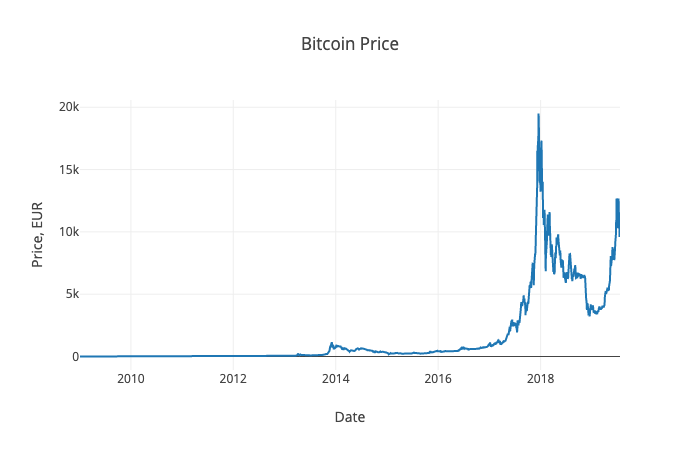
\includegraphics{0.png}
\end{figure}    
    
    \hypertarget{pull-kraken-btc-price-exchange-data}{%
\subsection{Pull Kraken BTC price exchange
data}\label{pull-kraken-btc-price-exchange-data}}

    Kraken is a cryptocurrency exchange in which market participants can
exchange various cryptocurrencies. It is one of the most reliable
exchanges ever, in fact until now it has never been breached.
\textbf{Kraken} was founded in 2011 in San Francisco and officially
started trading in 2013. It is owned by Payward Inc.~and is led by CEO
and co-founder Jesse Powell.

    It provides the easy movement of money to and from the participant's
linked bank accounts and the movement of encryptions to and from the
participant's digital wallets from the trading accounts linked to
Kraken.

    The BTC price from Kraken is downloaded using the Quandl API:

\emph{Daily Bitcoin exchange rate (BTC vs.~EUR) on Kraken. Updated daily
at 6:00 pm EST}

    \begin{Verbatim}[commandchars=\\\{\}]
{\color{incolor}In [{\color{incolor}13}]:} \PY{n}{btc\PYZus{}eur\PYZus{}price\PYZus{}kraken} \PY{o}{=} \PY{n}{quandl}\PY{o}{.}\PY{n}{get}\PY{p}{(}\PY{l+s+s2}{\PYZdq{}}\PY{l+s+s2}{BCHARTS/KRAKENEUR}\PY{l+s+s2}{\PYZdq{}}\PY{p}{,} 
                                           \PY{n}{start\PYZus{}date}\PY{o}{=}\PY{l+s+s2}{\PYZdq{}}\PY{l+s+s2}{2018\PYZhy{}01\PYZhy{}01}\PY{l+s+s2}{\PYZdq{}}\PY{p}{,} 
                                           \PY{n}{authtoken}\PY{o}{=}\PY{l+s+s2}{\PYZdq{}}\PY{l+s+s2}{CL4SbyNiw\PYZus{}NWebUiNoWA}\PY{l+s+s2}{\PYZdq{}}\PY{p}{)}
\end{Verbatim}

    \emph{btc\_eur\_price\_kraken\_} is the daily-price found in the OHLC
format. An OHLC chart is a type of chart typically used to illustrate
the movements in the price of a financial instrument over time and
indicate the open (\emph{Open}), the maximum (\emph{High}), the minimum
(\emph{Low}) and the close (\emph{Close}).

    Also in this case we are going to analyze the data from the dataframe.

    \begin{Verbatim}[commandchars=\\\{\}]
{\color{incolor}In [{\color{incolor}14}]:} \PY{n}{btc\PYZus{}eur\PYZus{}price\PYZus{}kraken}\PY{o}{.}\PY{n}{info}\PY{p}{(}\PY{p}{)}
\end{Verbatim}

    \begin{Verbatim}[commandchars=\\\{\}]
<class 'pandas.core.frame.DataFrame'>
DatetimeIndex: 567 entries, 2018-01-01 to 2019-07-21
Data columns (total 7 columns):
Open                 567 non-null float64
High                 567 non-null float64
Low                  567 non-null float64
Close                567 non-null float64
Volume (BTC)         567 non-null float64
Volume (Currency)    567 non-null float64
Weighted Price       567 non-null float64
dtypes: float64(7)
memory usage: 35.4 KB

    \end{Verbatim}

    In addition to \emph{Open}, \emph{High}, \emph{Low} and \emph{Close} we
also find the \emph{Volume} variable. The exchange volumes in technical
analysis are used to indicate the number of transactions carried out in
a specific period of time. They are very useful to understand how much a
crypto is used and therefore also indicate the strength of the market
behind the title.

    \hypertarget{weighted-price}{%
\subsubsection{Weighted Price}\label{weighted-price}}

    Another variable is \emph{Weighted Price}. In general a price-weighted
index is an index in which the member companies are weighted in
proportion to their price per share, rather than by number of shares
outstanding, market capitalization or other factors. In a price-weighted
index, stocks with higher prices receive a greater weight in the index,
regardless of the issuing company's actual size or the number of shares
outstanding.

    We consider the \emph{Weighted Price} because it is used as a trading
benchmark by investors who aim to be as passive as possible in their
execution, ensuring that the order is in line with the volume of the
market.

    \begin{Verbatim}[commandchars=\\\{\}]
{\color{incolor}In [{\color{incolor}15}]:} \PY{n}{btc\PYZus{}eur\PYZus{}price\PYZus{}kraken}\PY{o}{.}\PY{n}{describe}\PY{p}{(}\PY{p}{)}
\end{Verbatim}

\begin{Verbatim}[commandchars=\\\{\}]
{\color{outcolor}Out[{\color{outcolor}15}]:}                Open          High           Low         Close  Volume (BTC)  \textbackslash{}
         count    567.000000    567.000000    567.000000    567.000000    567.000000   
         mean    5997.238977   6178.148501   5762.107407   5977.371252   6781.432078   
         std     2269.035497   2369.603781   2039.471436   2193.905071   5195.298316   
         min        0.000000      0.000000      0.000000      0.000000      0.000000   
         25\%     4494.050000   4621.800000   4381.400000   4495.250000   3602.906056   
         50\%     5670.000000   5771.700000   5565.600000   5668.100000   5342.879384   
         75\%     7153.450000   7350.850000   6880.500000   7151.400000   8696.192449   
         max    20000.000000  20000.000000  13501.000000  14297.600000  51627.215385   
         
                Volume (Currency)  Weighted Price  
         count       5.670000e+02      567.000000  
         mean        4.318152e+07     5969.924976  
         std         4.022067e+07     2176.530885  
         min         0.000000e+00        0.000000  
         25\%         1.662019e+07     4511.448922  
         50\%         2.995900e+07     5655.395194  
         75\%         5.708206e+07     7127.862832  
         max         2.814326e+08    13906.517090  
\end{Verbatim}
            
    \begin{Verbatim}[commandchars=\\\{\}]
{\color{incolor}In [{\color{incolor}16}]:} \PY{n}{btc\PYZus{}eur\PYZus{}price\PYZus{}kraken}\PY{o}{.}\PY{n}{head}\PY{p}{(}\PY{l+m+mi}{10}\PY{p}{)}
\end{Verbatim}

\begin{Verbatim}[commandchars=\\\{\}]
{\color{outcolor}Out[{\color{outcolor}16}]:}                Open     High      Low    Close  Volume (BTC)  \textbackslash{}
         Date                                                           
         2018-01-01  11993.6  11995.2  11090.0  11350.0   3683.187439   
         2018-01-02  11359.1  12746.0  10905.0  12299.8   6820.728096   
         2018-01-03  12299.8  12887.0  12290.0  12660.0   4919.664762   
         2018-01-04  12643.3  12819.2  12000.0  12750.4   5884.940852   
         2018-01-05  12750.4  14480.0  12412.1  14297.6   6933.182531   
         2018-01-06  14297.4  14333.8  13501.0  14184.0   4159.696979   
         2018-01-07  14184.0  14199.7  13039.8  13237.2   3916.302169   
         2018-01-08  13208.6  13287.3  11605.0  12648.7   6843.762924   
         2018-01-09  12635.1  12768.6  11961.8  12072.9   5723.383169   
         2018-01-10  12072.9  12400.0  11200.0  12399.0   7541.680834   
         
                     Volume (Currency)  Weighted Price  
         Date                                           
         2018-01-01       4.234853e+07    11497.794756  
         2018-01-02       8.050079e+07    11802.375574  
         2018-01-03       6.184691e+07    12571.365849  
         2018-01-04       7.314782e+07    12429.661599  
         2018-01-05       9.287741e+07    13396.071726  
         2018-01-06       5.784690e+07    13906.517090  
         2018-01-07       5.312791e+07    13565.835201  
         2018-01-08       8.558162e+07    12505.053923  
         2018-01-09       7.089031e+07    12386.084568  
         2018-01-10       8.941647e+07    11856.305114  
\end{Verbatim}
            
    \begin{Verbatim}[commandchars=\\\{\}]
{\color{incolor}In [{\color{incolor}17}]:} \PY{n}{btc\PYZus{}eur\PYZus{}price\PYZus{}kraken}\PY{o}{.}\PY{n}{tail}\PY{p}{(}\PY{l+m+mi}{10}\PY{p}{)}
\end{Verbatim}

\begin{Verbatim}[commandchars=\\\{\}]
{\color{outcolor}Out[{\color{outcolor}17}]:}                Open     High     Low    Close  Volume (BTC)  \textbackslash{}
         Date                                                          
         2019-07-12  10088.3  10600.0  9850.0  10484.8   5730.516287   
         2019-07-13  10481.9  10514.3  9612.0  10125.0   5663.306135   
         2019-07-14  10125.0  10195.0  9199.0   9456.1   5722.412256   
         2019-07-15   9471.0   9848.9  8800.0   9633.6   8828.289949   
         2019-07-16   9651.0   9808.7  8350.9   8404.0  11815.108681   
         2019-07-17   8421.1   8905.0  8102.2   8644.4  11292.260413   
         2019-07-18   8648.7   9611.5  8275.6   9445.0  10353.226911   
         2019-07-19   9445.0   9583.6  9040.0   9395.2   6053.787487   
         2019-07-20   9393.1   9900.0  9241.0   9607.5   4195.909244   
         2019-07-21   9607.4   9671.8  9212.5   9437.3   3167.364132   
         
                     Volume (Currency)  Weighted Price  
         Date                                           
         2019-07-12       5.912859e+07    10318.195801  
         2019-07-13       5.678784e+07    10027.330026  
         2019-07-14       5.452587e+07     9528.475743  
         2019-07-15       8.195404e+07     9283.115868  
         2019-07-16       1.061665e+08     8985.659733  
         2019-07-17       9.631642e+07     8529.419110  
         2019-07-18       9.314096e+07     8996.321682  
         2019-07-19       5.619114e+07     9281.981387  
         2019-07-20       4.014711e+07     9568.153822  
         2019-07-21       2.979617e+07     9407.246048  
\end{Verbatim}
            
    We generate a graph considering the \emph{Weighted Price} column:

    \begin{Verbatim}[commandchars=\\\{\}]
{\color{incolor}In [{\color{incolor}18}]:} \PY{n}{btc\PYZus{}trace1} \PY{o}{=} \PY{n}{go}\PY{o}{.}\PY{n}{Scatter}\PY{p}{(}\PY{n}{x}\PY{o}{=}\PY{n}{btc\PYZus{}eur\PYZus{}price\PYZus{}kraken}\PY{o}{.}\PY{n}{index}\PY{p}{,} 
                                \PY{n}{y}\PY{o}{=}\PY{n}{btc\PYZus{}eur\PYZus{}price\PYZus{}kraken}\PY{p}{[}\PY{l+s+s1}{\PYZsq{}}\PY{l+s+s1}{Weighted Price}\PY{l+s+s1}{\PYZsq{}}\PY{p}{]}\PY{p}{)}
\end{Verbatim}

    \begin{Verbatim}[commandchars=\\\{\}]
{\color{incolor}In [{\color{incolor}19}]:} \PY{n}{data} \PY{o}{=} \PY{p}{[}\PY{n}{btc\PYZus{}trace1}\PY{p}{]}
         \PY{n}{layout} \PY{o}{=} \PY{n+nb}{dict}\PY{p}{(}\PY{n}{title} \PY{o}{=} \PY{l+s+s1}{\PYZsq{}}\PY{l+s+s1}{Weighted Price}\PY{l+s+s1}{\PYZsq{}}\PY{p}{,} \PY{n}{xaxis} \PY{o}{=} \PY{n+nb}{dict}\PY{p}{(}\PY{n}{title} \PY{o}{=} \PY{l+s+s1}{\PYZsq{}}\PY{l+s+s1}{Date}\PY{l+s+s1}{\PYZsq{}}\PY{p}{)}\PY{p}{,}
                       \PY{n}{yaxis} \PY{o}{=} \PY{n+nb}{dict}\PY{p}{(}\PY{n}{title} \PY{o}{=} \PY{l+s+s1}{\PYZsq{}}\PY{l+s+s1}{Price, EUR}\PY{l+s+s1}{\PYZsq{}}\PY{p}{)}\PY{p}{)}
         \PY{n}{fig} \PY{o}{=} \PY{n+nb}{dict}\PY{p}{(}\PY{n}{data}\PY{o}{=}\PY{n}{data}\PY{p}{,} \PY{n}{layout}\PY{o}{=}\PY{n}{layout}\PY{p}{)}
         \PY{n}{plotly}\PY{o}{.}\PY{n}{offline}\PY{o}{.}\PY{n}{iplot}\PY{p}{(}\PY{n}{fig}\PY{p}{)}
\end{Verbatim}

\begin{figure}[H]
	\centering
		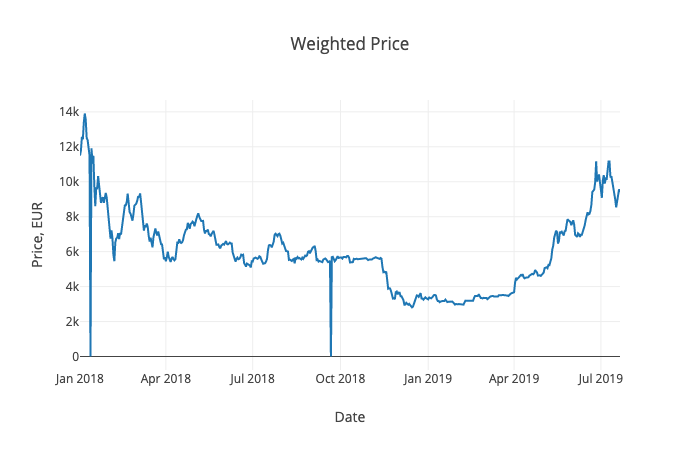
\includegraphics{1.png}
\end{figure}    
    
    We can see that there are irregularities certainly due to the failure to
update the Quandl dataset. We remove all the values 0, since we know
that the price of Bitcoin has never been equal to 0 in the times we are
examining.

    \begin{Verbatim}[commandchars=\\\{\}]
{\color{incolor}In [{\color{incolor}20}]:} \PY{n}{btc\PYZus{}eur\PYZus{}price\PYZus{}kraken}\PY{p}{[}\PY{l+s+s1}{\PYZsq{}}\PY{l+s+s1}{Weighted Price}\PY{l+s+s1}{\PYZsq{}}\PY{p}{]}\PY{o}{.}\PY{n}{replace}\PY{p}{(}\PY{l+m+mi}{0}\PY{p}{,} \PY{n}{np}\PY{o}{.}\PY{n}{nan}\PY{p}{,} \PY{n}{inplace}\PY{o}{=}\PY{k+kc}{True}\PY{p}{)}
         \PY{n}{btc\PYZus{}eur\PYZus{}price\PYZus{}kraken}\PY{p}{[}\PY{l+s+s1}{\PYZsq{}}\PY{l+s+s1}{Weighted Price}\PY{l+s+s1}{\PYZsq{}}\PY{p}{]}\PY{o}{.}\PY{n}{fillna}\PY{p}{(}\PY{n}{method}\PY{o}{=}\PY{l+s+s1}{\PYZsq{}}\PY{l+s+s1}{ffill}\PY{l+s+s1}{\PYZsq{}}\PY{p}{,} \PY{n}{inplace}\PY{o}{=}\PY{k+kc}{True}\PY{p}{)}
\end{Verbatim}

    When we plot again we will see a much cleaner graph without peaks.

    \begin{Verbatim}[commandchars=\\\{\}]
{\color{incolor}In [{\color{incolor}21}]:} \PY{n}{btc\PYZus{}trace2} \PY{o}{=} \PY{n}{go}\PY{o}{.}\PY{n}{Scatter}\PY{p}{(}\PY{n}{x}\PY{o}{=}\PY{n}{btc\PYZus{}eur\PYZus{}price\PYZus{}kraken}\PY{o}{.}\PY{n}{index}\PY{p}{,} 
                                \PY{n}{y}\PY{o}{=}\PY{n}{btc\PYZus{}eur\PYZus{}price\PYZus{}kraken}\PY{p}{[}\PY{l+s+s1}{\PYZsq{}}\PY{l+s+s1}{Weighted Price}\PY{l+s+s1}{\PYZsq{}}\PY{p}{]}\PY{p}{)}
\end{Verbatim}

    \begin{Verbatim}[commandchars=\\\{\}]
{\color{incolor}In [{\color{incolor}22}]:} \PY{n}{data} \PY{o}{=} \PY{p}{[}\PY{n}{btc\PYZus{}trace2}\PY{p}{]}
         \PY{n}{layout} \PY{o}{=} \PY{n+nb}{dict}\PY{p}{(}\PY{n}{title} \PY{o}{=} \PY{l+s+s1}{\PYZsq{}}\PY{l+s+s1}{Weighted Price}\PY{l+s+s1}{\PYZsq{}}\PY{p}{,} \PY{n}{xaxis} \PY{o}{=} \PY{n+nb}{dict}\PY{p}{(}\PY{n}{title} \PY{o}{=} \PY{l+s+s1}{\PYZsq{}}\PY{l+s+s1}{Date}\PY{l+s+s1}{\PYZsq{}}\PY{p}{)}\PY{p}{,}
                       \PY{n}{yaxis} \PY{o}{=} \PY{n+nb}{dict}\PY{p}{(}\PY{n}{title} \PY{o}{=} \PY{l+s+s1}{\PYZsq{}}\PY{l+s+s1}{Price, EUR}\PY{l+s+s1}{\PYZsq{}}\PY{p}{)}\PY{p}{)}
         \PY{n}{fig} \PY{o}{=} \PY{n+nb}{dict}\PY{p}{(}\PY{n}{data}\PY{o}{=}\PY{n}{data}\PY{p}{,} \PY{n}{layout}\PY{o}{=}\PY{n}{layout}\PY{p}{)}
         \PY{n}{plotly}\PY{o}{.}\PY{n}{offline}\PY{o}{.}\PY{n}{iplot}\PY{p}{(}\PY{n}{fig}\PY{p}{)}
\end{Verbatim}

\begin{figure}[H]
	\centering
		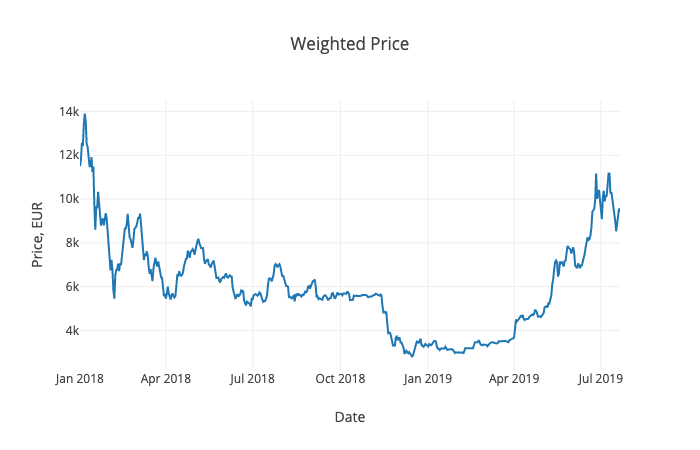
\includegraphics{2.png}
\end{figure}    
    
    A \textbf{correlation matrix} is a table showing the value of the
correlation coefficient between sets of variables (correlation
coefficients are used in statistics to measure how strong a relationship
is between two variables ).

    This analysis allows you to see which pairs have the highest
correlation, the pairs which are highly correlated represent the same
variance of the dataset thus we can further analyze them to understand
which attribute among the pairs are most significant for building the
model. This plot shows you which variables are correlated to each other
from a scale already predefined.

    Below we find the correlation matrix of our initial dataset
``btc\_eur\_price\_kraken'':

    \begin{Verbatim}[commandchars=\\\{\}]
{\color{incolor}In [{\color{incolor}23}]:} \PY{n}{sns}\PY{o}{.}\PY{n}{heatmap}\PY{p}{(}\PY{n}{btc\PYZus{}eur\PYZus{}price\PYZus{}kraken}\PY{o}{.}\PY{n}{corr}\PY{p}{(}\PY{p}{)}\PY{p}{,} \PY{n}{annot}\PY{o}{=}\PY{k+kc}{True}\PY{p}{,} 
                     \PY{n}{cmap}\PY{o}{=}\PY{l+s+s1}{\PYZsq{}}\PY{l+s+s1}{RdYlGn}\PY{l+s+s1}{\PYZsq{}}\PY{p}{,} \PY{n}{linewidths}\PY{o}{=}\PY{l+m+mf}{0.5}\PY{p}{,} \PY{n}{vmin}\PY{o}{=}\PY{l+m+mi}{0}\PY{p}{)}
         \PY{n}{plt}\PY{o}{.}\PY{n}{show}\PY{p}{(}\PY{p}{)}
\end{Verbatim}

    \begin{center}
    \adjustimage{max size={0.9\linewidth}{0.9\paperheight}}{output_58_0.png}
    \end{center}
    { \hspace*{\fill} \\}
    
    From our correlation matrix we can understand that \emph{Volume} is
correlated to \emph{Weighted Price}. \emph{Open}, \emph{High},
\emph{Low} and \emph{Close} are directly related to \emph{Weighted
Price}.

    Below is the code to plot the univariate distribution of the numerical
columns which contains the histograms and the estimated PDF. We use
displot of the seaborn library to plot this graph:

    \begin{Verbatim}[commandchars=\\\{\}]
{\color{incolor}In [{\color{incolor}24}]:} \PY{n}{col\PYZus{}names} \PY{o}{=} \PY{p}{[}\PY{l+s+s1}{\PYZsq{}}\PY{l+s+s1}{Open}\PY{l+s+s1}{\PYZsq{}}\PY{p}{,}\PY{l+s+s1}{\PYZsq{}}\PY{l+s+s1}{High}\PY{l+s+s1}{\PYZsq{}}\PY{p}{,} \PY{l+s+s1}{\PYZsq{}}\PY{l+s+s1}{Low}\PY{l+s+s1}{\PYZsq{}}\PY{p}{,} \PY{l+s+s1}{\PYZsq{}}\PY{l+s+s1}{Close}\PY{l+s+s1}{\PYZsq{}}\PY{p}{,} 
                      \PY{l+s+s1}{\PYZsq{}}\PY{l+s+s1}{Volume (BTC)}\PY{l+s+s1}{\PYZsq{}}\PY{p}{,} \PY{l+s+s1}{\PYZsq{}}\PY{l+s+s1}{Volume (Currency)}\PY{l+s+s1}{\PYZsq{}}\PY{p}{,} 
                      \PY{l+s+s1}{\PYZsq{}}\PY{l+s+s1}{Weighted Price}\PY{l+s+s1}{\PYZsq{}}\PY{p}{]}
\end{Verbatim}

    \begin{Verbatim}[commandchars=\\\{\}]
{\color{incolor}In [{\color{incolor}25}]:} \PY{n}{fig}\PY{p}{,} \PY{n}{ax} \PY{o}{=} \PY{n}{plt}\PY{o}{.}\PY{n}{subplots}\PY{p}{(}\PY{n+nb}{len}\PY{p}{(}\PY{n}{col\PYZus{}names}\PY{p}{)}\PY{p}{,} \PY{n}{figsize}\PY{o}{=}\PY{p}{(}\PY{l+m+mi}{20}\PY{p}{,}\PY{l+m+mi}{15}\PY{p}{)}\PY{p}{)}
         
         \PY{k}{for} \PY{n}{i}\PY{p}{,} \PY{n}{col\PYZus{}val} \PY{o+ow}{in} \PY{n+nb}{enumerate}\PY{p}{(}\PY{n}{col\PYZus{}names}\PY{p}{)}\PY{p}{:}
         
             \PY{n}{sns}\PY{o}{.}\PY{n}{distplot}\PY{p}{(}\PY{n}{btc\PYZus{}eur\PYZus{}price\PYZus{}kraken}\PY{p}{[}\PY{n}{col\PYZus{}val}\PY{p}{]}\PY{p}{,} \PY{n}{hist}\PY{o}{=}\PY{k+kc}{True}\PY{p}{,} \PY{n}{ax}\PY{o}{=}\PY{n}{ax}\PY{p}{[}\PY{n}{i}\PY{p}{]}\PY{p}{)}
             \PY{n}{ax}\PY{p}{[}\PY{n}{i}\PY{p}{]}\PY{o}{.}\PY{n}{set\PYZus{}xlabel}\PY{p}{(}\PY{n}{col\PYZus{}val}\PY{p}{,} \PY{n}{fontsize}\PY{o}{=}\PY{l+m+mi}{15}\PY{p}{)}
             \PY{n}{ax}\PY{p}{[}\PY{n}{i}\PY{p}{]}\PY{o}{.}\PY{n}{set\PYZus{}ylabel}\PY{p}{(}\PY{l+s+s1}{\PYZsq{}}\PY{l+s+s1}{Count}\PY{l+s+s1}{\PYZsq{}}\PY{p}{,} \PY{n}{fontsize}\PY{o}{=}\PY{l+m+mi}{15}\PY{p}{)}
         
         \PY{n}{fig}\PY{o}{.}\PY{n}{tight\PYZus{}layout}\PY{p}{(}\PY{p}{)}
         \PY{n}{plt}\PY{o}{.}\PY{n}{show}\PY{p}{(}\PY{p}{)}
\end{Verbatim}

    \begin{center}
    \adjustimage{max size={0.9\linewidth}{0.9\paperheight}}{output_62_0.png}
    \end{center}
    { \hspace*{\fill} \\}
    
    An outlier might indicate a mistake in the data (like a typo, or a
measuring error, seasonal effects etc), in which case it should be
corrected or removed from the data before calculating summary statistics
or deriving insights from the data, failing to which will lead to
incorrect analysis.

    Below is the code to plot the boxplot of all the column names mentioned
in the list \emph{col\_names}. A boxplot is a standardized way of
displaying the distribution of data based on a five number summary:

\begin{itemize}
\item
  median (Q2/50th Percentile): the middle value of the dataset.
\item
  first quartile (Q1/25th Percentile): the middle number between the
  smallest number (not the ``minimum'') and the median of the dataset.
\item
  third quartile (Q3/75th Percentile): the middle value between the
  median and the highest value (not the ``maximum'') of the dataset.
\item
  maximum: Q3 + 1.5*IQR
\item
  minimum: Q1 - 1.5*IQR
\end{itemize}

IQR: 25th to the 75th percentile
\begin{figure}[H]
	\centering
		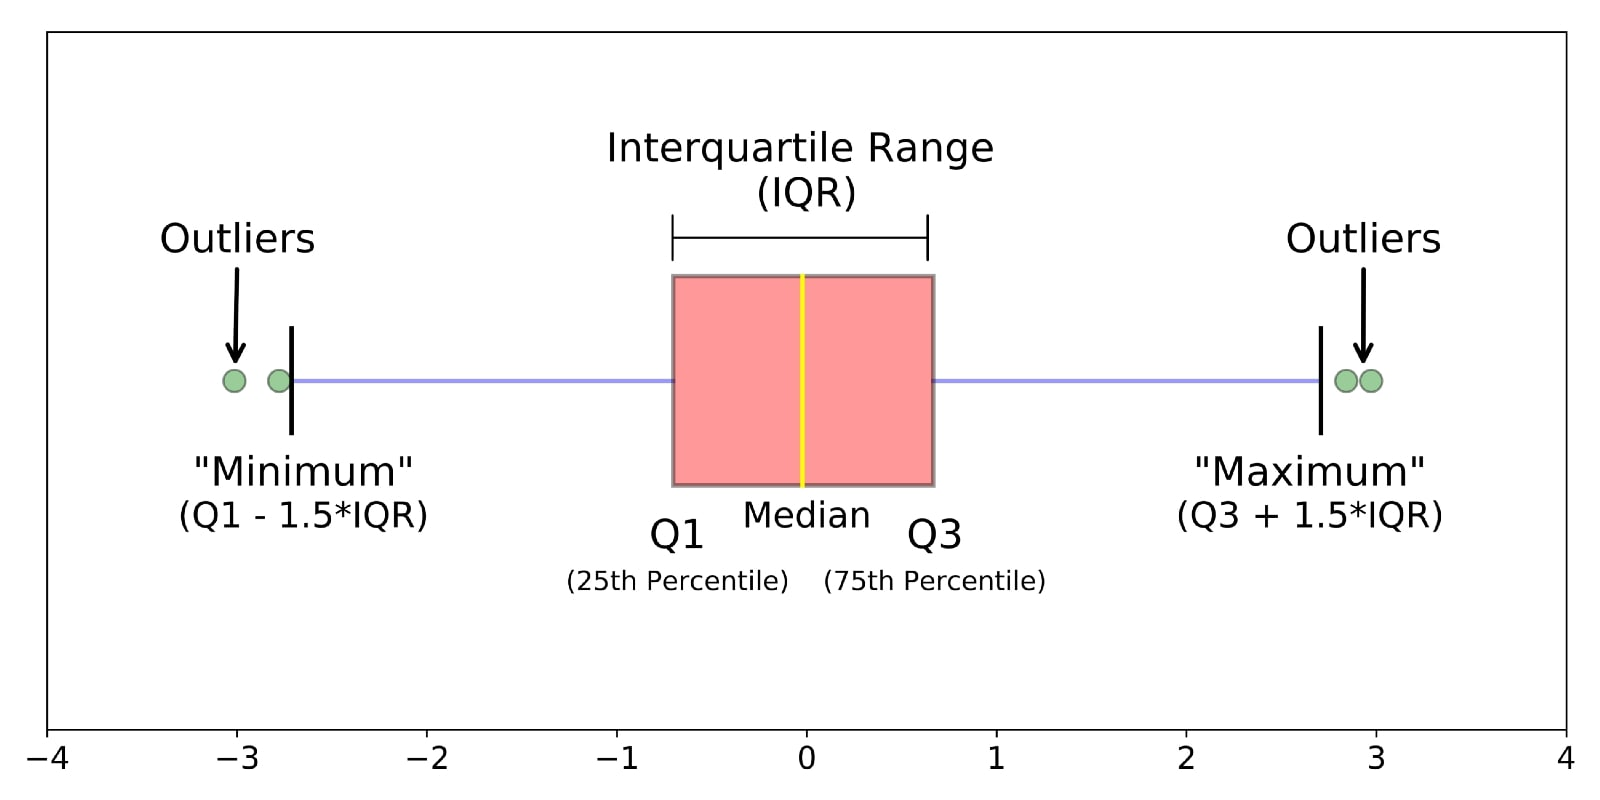
\includegraphics{boxplot.jpg}
		  \caption{Figure 1: Different parts of a boxplot}
\end{figure}

    \begin{Verbatim}[commandchars=\\\{\}]
{\color{incolor}In [{\color{incolor}26}]:} \PY{n}{fig}\PY{p}{,} \PY{n}{ax} \PY{o}{=} \PY{n}{plt}\PY{o}{.}\PY{n}{subplots}\PY{p}{(}\PY{n+nb}{len}\PY{p}{(}\PY{n}{col\PYZus{}names}\PY{p}{)}\PY{p}{,} \PY{n}{figsize}\PY{o}{=}\PY{p}{(}\PY{l+m+mi}{15}\PY{p}{,}\PY{l+m+mi}{25}\PY{p}{)}\PY{p}{)}
         
         \PY{k}{for} \PY{n}{i}\PY{p}{,} \PY{n}{col\PYZus{}val} \PY{o+ow}{in} \PY{n+nb}{enumerate}\PY{p}{(}\PY{n}{col\PYZus{}names}\PY{p}{)}\PY{p}{:}
         
             \PY{n}{sns}\PY{o}{.}\PY{n}{boxplot}\PY{p}{(}\PY{n}{y}\PY{o}{=}\PY{n}{btc\PYZus{}eur\PYZus{}price\PYZus{}kraken}\PY{p}{[}\PY{n}{col\PYZus{}val}\PY{p}{]}\PY{p}{,} \PY{n}{ax}\PY{o}{=}\PY{n}{ax}\PY{p}{[}\PY{n}{i}\PY{p}{]}\PY{p}{)}
             
             \PY{n}{ax}\PY{p}{[}\PY{n}{i}\PY{p}{]}\PY{o}{.}\PY{n}{set\PYZus{}title}\PY{p}{(}\PY{n}{col\PYZus{}val}\PY{p}{,} \PY{n}{fontsize}\PY{o}{=}\PY{l+m+mi}{10}\PY{p}{)}
             \PY{n}{ax}\PY{p}{[}\PY{n}{i}\PY{p}{]}\PY{o}{.}\PY{n}{set\PYZus{}ylabel}\PY{p}{(}\PY{l+s+s1}{\PYZsq{}}\PY{l+s+s1}{Value}\PY{l+s+s1}{\PYZsq{}}\PY{p}{,} \PY{n}{fontsize}\PY{o}{=}\PY{l+m+mi}{10}\PY{p}{)}
         
         \PY{n}{plt}\PY{o}{.}\PY{n}{show}\PY{p}{(}\PY{p}{)}
\end{Verbatim}

    \begin{center}
    \adjustimage{max size={0.9\linewidth}{0.9\paperheight}}{output_66_0.png}
    \end{center}
    { \hspace*{\fill} \\}
    
    In our case the outliers are not due to ``errors'', they are simply
``rare'' values that BTC has assumed. So they should not be removed, but
to get an idea on how to delete these values, we will identify them
using the \textbf{Interquartile Range Rule} and then go and create a new
dataset without an outlier.

    \begin{Verbatim}[commandchars=\\\{\}]
{\color{incolor}In [{\color{incolor}27}]:} \PY{n}{df} \PY{o}{=} \PY{n}{pd}\PY{o}{.}\PY{n}{DataFrame}\PY{p}{(}\PY{n}{btc\PYZus{}eur\PYZus{}price\PYZus{}kraken}\PY{p}{,} 
                          \PY{n}{index} \PY{o}{=} \PY{n}{btc\PYZus{}eur\PYZus{}price\PYZus{}kraken}\PY{o}{.}\PY{n}{index}\PY{p}{,} \PY{n}{columns} \PY{o}{=} \PY{n}{col\PYZus{}names}\PY{p}{)}
         
         \PY{n}{outlier\PYZus{}rang\PYZus{}max}\PY{p}{,} \PY{n}{outlier\PYZus{}rang\PYZus{}min} \PY{o}{=} \PY{n+nb}{dict}\PY{p}{(}\PY{p}{)}\PY{p}{,} \PY{n+nb}{dict}\PY{p}{(}\PY{p}{)}
         
         \PY{n}{df\PYZus{}description} \PY{o}{=} \PY{n}{df}\PY{o}{.}\PY{n}{describe}\PY{p}{(}\PY{p}{)}
         \PY{k}{for} \PY{n}{col\PYZus{}name} \PY{o+ow}{in} \PY{n}{col\PYZus{}names}\PY{p}{:}
             \PY{n}{q1} \PY{o}{=} \PY{n}{df\PYZus{}description}\PY{p}{[}\PY{n}{col\PYZus{}name}\PY{p}{]}\PY{p}{[}\PY{l+s+s1}{\PYZsq{}}\PY{l+s+s1}{25}\PY{l+s+s1}{\PYZpc{}}\PY{l+s+s1}{\PYZsq{}}\PY{p}{]}
             \PY{n}{q3} \PY{o}{=} \PY{n}{df\PYZus{}description}\PY{p}{[}\PY{n}{col\PYZus{}name}\PY{p}{]}\PY{p}{[}\PY{l+s+s1}{\PYZsq{}}\PY{l+s+s1}{75}\PY{l+s+s1}{\PYZpc{}}\PY{l+s+s1}{\PYZsq{}}\PY{p}{]}
             \PY{n}{iqr} \PY{o}{=} \PY{n}{q3}\PY{o}{\PYZhy{}}\PY{n}{q1}
             \PY{n}{fence\PYZus{}low} \PY{o}{=} \PY{n}{q1}\PY{o}{\PYZhy{}}\PY{l+m+mf}{1.5}\PY{o}{*}\PY{n}{iqr}
             \PY{n}{outlier\PYZus{}rang\PYZus{}min}\PY{p}{[}\PY{n}{col\PYZus{}name}\PY{p}{]} \PY{o}{=} \PY{n}{fence\PYZus{}low}
             \PY{n}{fence\PYZus{}high} \PY{o}{=} \PY{n}{q3}\PY{o}{+}\PY{l+m+mf}{1.5}\PY{o}{*}\PY{n}{iqr}
             \PY{n}{outlier\PYZus{}rang\PYZus{}max}\PY{p}{[}\PY{n}{col\PYZus{}name}\PY{p}{]} \PY{o}{=} \PY{n}{fence\PYZus{}high}
         
         \PY{k}{def} \PY{n+nf}{remove\PYZus{}outlier}\PY{p}{(}\PY{n}{df\PYZus{}in}\PY{p}{,} \PY{n}{col\PYZus{}names}\PY{p}{)}\PY{p}{:}
             \PY{n}{q1} \PY{o}{=} \PY{n}{df\PYZus{}in}\PY{p}{[}\PY{n}{col\PYZus{}names}\PY{p}{]}\PY{o}{.}\PY{n}{quantile}\PY{p}{(}\PY{l+m+mf}{0.25}\PY{p}{)}
             \PY{n}{q3} \PY{o}{=} \PY{n}{df\PYZus{}in}\PY{p}{[}\PY{n}{col\PYZus{}names}\PY{p}{]}\PY{o}{.}\PY{n}{quantile}\PY{p}{(}\PY{l+m+mf}{0.75}\PY{p}{)}
             \PY{n}{iqr} \PY{o}{=} \PY{n}{q3}\PY{o}{\PYZhy{}}\PY{n}{q1}
             \PY{n}{fence\PYZus{}low}  \PY{o}{=} \PY{n}{q1}\PY{o}{\PYZhy{}}\PY{l+m+mf}{1.5}\PY{o}{*}\PY{n}{iqr}
             \PY{n}{fence\PYZus{}high} \PY{o}{=} \PY{n}{q3}\PY{o}{+}\PY{l+m+mf}{1.5}\PY{o}{*}\PY{n}{iqr}
             \PY{n}{df\PYZus{}out} \PY{o}{=} \PY{n}{df\PYZus{}in}\PY{o}{.}\PY{n}{loc}\PY{p}{[}\PY{p}{(}\PY{n}{df\PYZus{}in}\PY{p}{[}\PY{n}{col\PYZus{}names}\PY{p}{]} \PY{o}{\PYZgt{}} \PY{n}{fence\PYZus{}low}\PY{p}{)} 
                                \PY{o}{\PYZam{}} \PY{p}{(}\PY{n}{df\PYZus{}in}\PY{p}{[}\PY{n}{col\PYZus{}names}\PY{p}{]} \PY{o}{\PYZlt{}} \PY{n}{fence\PYZus{}high}\PY{p}{)}\PY{p}{]}
             \PY{k}{return} \PY{n}{df\PYZus{}out}
         
         \PY{n}{filtered} \PY{o}{=} \PY{n}{df}\PY{o}{.}\PY{n}{apply}\PY{p}{(}\PY{k}{lambda} \PY{n}{x} \PY{p}{:} \PY{n}{x}\PY{p}{[}\PY{p}{(}\PY{n}{x}\PY{o}{.}\PY{n}{values} \PY{o}{\PYZgt{}} \PY{n}{outlier\PYZus{}rang\PYZus{}min}\PY{p}{[}\PY{n}{x}\PY{o}{.}\PY{n}{name}\PY{p}{]}\PY{p}{)} 
                                          \PY{o}{\PYZam{}} \PY{p}{(}\PY{n}{x}\PY{o}{.}\PY{n}{values} \PY{o}{\PYZlt{}} \PY{n}{outlier\PYZus{}rang\PYZus{}max}\PY{p}{[}\PY{n}{x}\PY{o}{.}\PY{n}{name}\PY{p}{]}\PY{p}{)}\PY{p}{]}\PY{p}{,}
                             \PY{n}{axis} \PY{o}{=} \PY{l+m+mi}{0}\PY{p}{)}
\end{Verbatim}

    Here is the number of outliers eliminated:

    \begin{Verbatim}[commandchars=\\\{\}]
{\color{incolor}In [{\color{incolor}28}]:} \PY{n}{filtered}\PY{o}{.}\PY{n}{isna}\PY{p}{(}\PY{p}{)}\PY{o}{.}\PY{n}{sum}\PY{p}{(}\PY{p}{)}
\end{Verbatim}

\begin{Verbatim}[commandchars=\\\{\}]
{\color{outcolor}Out[{\color{outcolor}28}]:} Open                 18
         High                 20
         Low                  15
         Close                17
         Volume (BTC)         27
         Volume (Currency)    31
         Weighted Price       18
         dtype: int64
\end{Verbatim}
            
    We create a new dataset without outlier and let's trace the graph of the
\emph{Weighted Price} column.

    \begin{Verbatim}[commandchars=\\\{\}]
{\color{incolor}In [{\color{incolor}29}]:} \PY{n}{new} \PY{o}{=} \PY{n}{filtered}\PY{o}{.}\PY{n}{copy}\PY{p}{(}\PY{p}{)}
\end{Verbatim}

    \begin{Verbatim}[commandchars=\\\{\}]
{\color{incolor}In [{\color{incolor}30}]:} \PY{n}{btc\PYZus{}trace3} \PY{o}{=} \PY{n}{go}\PY{o}{.}\PY{n}{Scatter}\PY{p}{(}\PY{n}{x}\PY{o}{=}\PY{n}{new}\PY{o}{.}\PY{n}{index}\PY{p}{,} 
                                 \PY{n}{y}\PY{o}{=}\PY{n}{new}\PY{p}{[}\PY{l+s+s1}{\PYZsq{}}\PY{l+s+s1}{Weighted Price}\PY{l+s+s1}{\PYZsq{}}\PY{p}{]}\PY{p}{)}
\end{Verbatim}

    \begin{Verbatim}[commandchars=\\\{\}]
{\color{incolor}In [{\color{incolor}31}]:} \PY{n}{data} \PY{o}{=} \PY{p}{[}\PY{n}{btc\PYZus{}trace3}\PY{p}{]}
         \PY{n}{layout} \PY{o}{=} \PY{n+nb}{dict}\PY{p}{(}\PY{n}{title} \PY{o}{=} \PY{l+s+s1}{\PYZsq{}}\PY{l+s+s1}{Weighted Price}\PY{l+s+s1}{\PYZsq{}}\PY{p}{,} \PY{n}{xaxis} \PY{o}{=} \PY{n+nb}{dict}\PY{p}{(}\PY{n}{title} \PY{o}{=} \PY{l+s+s1}{\PYZsq{}}\PY{l+s+s1}{Date}\PY{l+s+s1}{\PYZsq{}}\PY{p}{)}\PY{p}{,}
                       \PY{n}{yaxis} \PY{o}{=} \PY{n+nb}{dict}\PY{p}{(}\PY{n}{title} \PY{o}{=} \PY{l+s+s1}{\PYZsq{}}\PY{l+s+s1}{Price, EUR}\PY{l+s+s1}{\PYZsq{}}\PY{p}{)}\PY{p}{)}
         \PY{n}{fig} \PY{o}{=} \PY{n+nb}{dict}\PY{p}{(}\PY{n}{data}\PY{o}{=}\PY{n}{data}\PY{p}{,} \PY{n}{layout}\PY{o}{=}\PY{n}{layout}\PY{p}{)}
         \PY{n}{plotly}\PY{o}{.}\PY{n}{offline}\PY{o}{.}\PY{n}{iplot}\PY{p}{(}\PY{n}{fig}\PY{p}{)}
\end{Verbatim}

\begin{figure}[H]
	\centering
		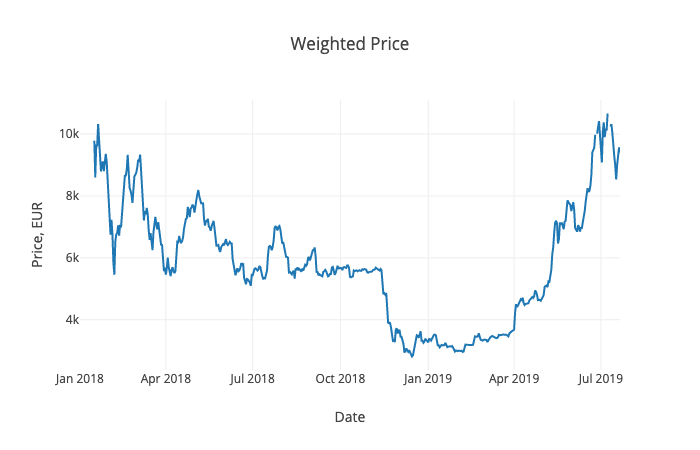
\includegraphics{3.png}
\end{figure}    
    
    \textbf{Candlestick Charts} are a type of financial chart for tracking
the movement of securities. Candlesticks are so named because the
rectangular shape and lines on either end resemble a candle with wicks.

Each candlestick represents one day's worth of price data about a stock
through four pieces of information: the opening price, the closing
price, the high price, and the low price. The color of the central
rectangle (called the real body) tells investors whether the opening
price or the closing price was higher.

    We plot our candlestick chart by taking the ``Open'', ``High'', ``Low''
and ``Close'' columns of our new dataset.

    \begin{Verbatim}[commandchars=\\\{\}]
{\color{incolor}In [{\color{incolor}32}]:} \PY{n}{trace1} \PY{o}{=} \PY{n}{go}\PY{o}{.}\PY{n}{Candlestick}\PY{p}{(}\PY{n}{x}\PY{o}{=}\PY{n}{new}\PY{o}{.}\PY{n}{index}\PY{p}{,}
                         \PY{n+nb}{open}\PY{o}{=}\PY{n}{new}\PY{p}{[}\PY{l+s+s1}{\PYZsq{}}\PY{l+s+s1}{Open}\PY{l+s+s1}{\PYZsq{}}\PY{p}{]}\PY{p}{,}
                         \PY{n}{high}\PY{o}{=}\PY{n}{new}\PY{p}{[}\PY{l+s+s1}{\PYZsq{}}\PY{l+s+s1}{High}\PY{l+s+s1}{\PYZsq{}}\PY{p}{]}\PY{p}{,}
                         \PY{n}{low}\PY{o}{=}\PY{n}{new}\PY{p}{[}\PY{l+s+s1}{\PYZsq{}}\PY{l+s+s1}{Low}\PY{l+s+s1}{\PYZsq{}}\PY{p}{]}\PY{p}{,}
                         \PY{n}{close}\PY{o}{=}\PY{n}{new}\PY{p}{[}\PY{l+s+s1}{\PYZsq{}}\PY{l+s+s1}{Close}\PY{l+s+s1}{\PYZsq{}}\PY{p}{]}\PY{p}{,}\PY{p}{)}                
\end{Verbatim}

    \begin{Verbatim}[commandchars=\\\{\}]
{\color{incolor}In [{\color{incolor}33}]:} \PY{n}{data1} \PY{o}{=} \PY{p}{[}\PY{n}{trace1}\PY{p}{]}
         \PY{n}{layout} \PY{o}{=} \PY{p}{\PYZob{}}
             \PY{l+s+s1}{\PYZsq{}}\PY{l+s+s1}{title}\PY{l+s+s1}{\PYZsq{}}\PY{p}{:} \PY{l+s+s1}{\PYZsq{}}\PY{l+s+s1}{Candlestick}\PY{l+s+s1}{\PYZsq{}}\PY{p}{,}
             \PY{l+s+s1}{\PYZsq{}}\PY{l+s+s1}{yaxis}\PY{l+s+s1}{\PYZsq{}}\PY{p}{:} \PY{p}{\PYZob{}}\PY{l+s+s1}{\PYZsq{}}\PY{l+s+s1}{title}\PY{l+s+s1}{\PYZsq{}}\PY{p}{:} \PY{l+s+s1}{\PYZsq{}}\PY{l+s+s1}{Price (EUR)}\PY{l+s+s1}{\PYZsq{}}\PY{p}{\PYZcb{}}\PY{p}{,}
             \PY{l+s+s1}{\PYZsq{}}\PY{l+s+s1}{xaxis}\PY{l+s+s1}{\PYZsq{}}\PY{p}{:} \PY{p}{\PYZob{}}\PY{l+s+s1}{\PYZsq{}}\PY{l+s+s1}{title}\PY{l+s+s1}{\PYZsq{}}\PY{p}{:} \PY{l+s+s1}{\PYZsq{}}\PY{l+s+s1}{Date}\PY{l+s+s1}{\PYZsq{}}\PY{p}{\PYZcb{}}\PY{p}{,}
         \PY{p}{\PYZcb{}}
         \PY{n}{fig} \PY{o}{=} \PY{n+nb}{dict}\PY{p}{(}\PY{n}{data}\PY{o}{=}\PY{n}{data1}\PY{p}{,} \PY{n}{layout}\PY{o}{=}\PY{n}{layout}\PY{p}{)}
         \PY{n}{plotly}\PY{o}{.}\PY{n}{offline}\PY{o}{.}\PY{n}{iplot}\PY{p}{(}\PY{n}{fig}\PY{p}{,} \PY{n}{filename}\PY{o}{=}\PY{l+s+s1}{\PYZsq{}}\PY{l+s+s1}{candlestick}\PY{l+s+s1}{\PYZsq{}}\PY{p}{)}
\end{Verbatim}

\begin{figure}[H]
	\centering
		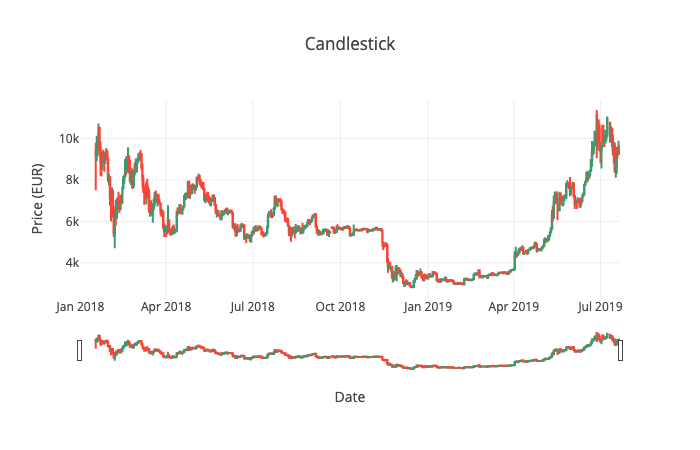
\includegraphics{4.png}
\end{figure}    
    
    \hypertarget{pull-pricing-data-for-one-more-btc-exchange}{%
\subsection{Pull pricing data for one more BTC
exchange}\label{pull-pricing-data-for-one-more-btc-exchange}}

    The nature of Bitcoin exchanges is that the pricing is determined by
supply and demand, hence no single exchange contains a true ``master
price'' of Bitcoin. To solve this issue we will pull data from one more
major Bitcoin exchange to calculate an aggregate Bitcoin price index.

    Let's analyze now the \emph{Weighted Price} data for one more BTC
exchange and our dataset without outliers. The exchange in question is
\textbf{Bitstamp} and we always find it on Quandl. Founded in 2011,
Bitstamp is the world's foremost Bitcoin exchange, providing customers
with an easy to use, secure and reliable service.

    We will download the data from each exchange into a dictionary of
dataframes:

    \begin{Verbatim}[commandchars=\\\{\}]
{\color{incolor}In [{\color{incolor}34}]:} \PY{n}{exchanges} \PY{o}{=} \PY{p}{[}\PY{l+s+s1}{\PYZsq{}}\PY{l+s+s1}{BITSTAMP}\PY{l+s+s1}{\PYZsq{}}\PY{p}{,}\PY{p}{]}
         
         \PY{n}{exchange\PYZus{}data} \PY{o}{=} \PY{p}{\PYZob{}}\PY{p}{\PYZcb{}}
         \PY{n}{exchange\PYZus{}data}\PY{p}{[}\PY{l+s+s1}{\PYZsq{}}\PY{l+s+s1}{KRAKEN}\PY{l+s+s1}{\PYZsq{}}\PY{p}{]} \PY{o}{=} \PY{n}{btc\PYZus{}eur\PYZus{}price\PYZus{}kraken}
         
         \PY{k}{for} \PY{n}{exchange} \PY{o+ow}{in} \PY{n}{exchanges}\PY{p}{:}
             \PY{n}{exchange\PYZus{}code} \PY{o}{=} \PY{l+s+s1}{\PYZsq{}}\PY{l+s+s1}{BCHARTS/}\PY{l+s+si}{\PYZob{}\PYZcb{}}\PY{l+s+s1}{EUR}\PY{l+s+s1}{\PYZsq{}}\PY{o}{.}\PY{n}{format}\PY{p}{(}\PY{n}{exchange}\PY{p}{)}
             \PY{n}{btc\PYZus{}exchange\PYZus{}df} \PY{o}{=} \PY{n}{quandl}\PY{o}{.}\PY{n}{get}\PY{p}{(}\PY{l+s+s2}{\PYZdq{}}\PY{l+s+s2}{BCHARTS/BITSTAMPEUR}\PY{l+s+s2}{\PYZdq{}}\PY{p}{,}
                                          \PY{n}{start\PYZus{}date}\PY{o}{=}\PY{l+s+s2}{\PYZdq{}}\PY{l+s+s2}{2018\PYZhy{}01\PYZhy{}01}\PY{l+s+s2}{\PYZdq{}}\PY{p}{,}
                                          \PY{n}{authtoken}\PY{o}{=}\PY{l+s+s2}{\PYZdq{}}\PY{l+s+s2}{CL4SbyNiw\PYZus{}NWebUiNoWA}\PY{l+s+s2}{\PYZdq{}}\PY{p}{)}
             \PY{n}{exchange\PYZus{}data}\PY{p}{[}\PY{n}{exchange}\PY{p}{]} \PY{o}{=} \PY{n}{btc\PYZus{}exchange\PYZus{}df}
         \PY{n}{btc\PYZus{}exchange\PYZus{}df}\PY{p}{[}\PY{l+s+s1}{\PYZsq{}}\PY{l+s+s1}{Weighted Price}\PY{l+s+s1}{\PYZsq{}}\PY{p}{]}\PY{o}{.}\PY{n}{replace}\PY{p}{(}\PY{l+m+mi}{0}\PY{p}{,} \PY{n}{np}\PY{o}{.}\PY{n}{nan}\PY{p}{,} \PY{n}{inplace}\PY{o}{=}\PY{k+kc}{True}\PY{p}{)}
         \PY{n}{btc\PYZus{}exchange\PYZus{}df}\PY{p}{[}\PY{l+s+s1}{\PYZsq{}}\PY{l+s+s1}{Weighted Price}\PY{l+s+s1}{\PYZsq{}}\PY{p}{]}\PY{o}{.}\PY{n}{fillna}\PY{p}{(}\PY{n}{method}\PY{o}{=}\PY{l+s+s1}{\PYZsq{}}\PY{l+s+s1}{ffill}\PY{l+s+s1}{\PYZsq{}}\PY{p}{,} \PY{n}{inplace}\PY{o}{=}\PY{k+kc}{True}\PY{p}{)}
\end{Verbatim}

    We will define a simple function to merge a common column of each
dataframe into a new combined dataframe:

    \begin{Verbatim}[commandchars=\\\{\}]
{\color{incolor}In [{\color{incolor}35}]:} \PY{k}{def} \PY{n+nf}{merge\PYZus{}dfs\PYZus{}on\PYZus{}column}\PY{p}{(}\PY{n}{dataframes}\PY{p}{,} \PY{n}{labels}\PY{p}{,} \PY{n}{col}\PY{p}{)}\PY{p}{:}
             \PY{n}{series\PYZus{}dict} \PY{o}{=} \PY{p}{\PYZob{}}\PY{p}{\PYZcb{}}
             \PY{k}{for} \PY{n}{index} \PY{o+ow}{in} \PY{n+nb}{range}\PY{p}{(}\PY{n+nb}{len}\PY{p}{(}\PY{n}{dataframes}\PY{p}{)}\PY{p}{)}\PY{p}{:}
                 \PY{n}{series\PYZus{}dict}\PY{p}{[}\PY{n}{labels}\PY{p}{[}\PY{n}{index}\PY{p}{]}\PY{p}{]} \PY{o}{=} \PY{n}{dataframes}\PY{p}{[}\PY{n}{index}\PY{p}{]}\PY{p}{[}\PY{n}{col}\PY{p}{]}
                 
             \PY{k}{return} \PY{n}{pd}\PY{o}{.}\PY{n}{DataFrame}\PY{p}{(}\PY{n}{series\PYZus{}dict}\PY{p}{)}
\end{Verbatim}

    Now we will merge all of the dataframes together on their \emph{Weighted
Price} column.

    \begin{Verbatim}[commandchars=\\\{\}]
{\color{incolor}In [{\color{incolor}36}]:} \PY{n}{btc\PYZus{}eur\PYZus{}datasets} \PY{o}{=} \PY{n}{merge\PYZus{}dfs\PYZus{}on\PYZus{}column}\PY{p}{(}\PY{n+nb}{list}\PY{p}{(}\PY{n}{exchange\PYZus{}data}\PY{o}{.}\PY{n}{values}\PY{p}{(}\PY{p}{)}\PY{p}{)}\PY{p}{,}
                                                \PY{n+nb}{list}\PY{p}{(}\PY{n}{exchange\PYZus{}data}\PY{o}{.}\PY{n}{keys}\PY{p}{(}\PY{p}{)}\PY{p}{)}\PY{p}{,}
                                                \PY{l+s+s1}{\PYZsq{}}\PY{l+s+s1}{Weighted Price}\PY{l+s+s1}{\PYZsq{}}\PY{p}{)}
\end{Verbatim}

    \begin{Verbatim}[commandchars=\\\{\}]
{\color{incolor}In [{\color{incolor}37}]:} \PY{n}{btc\PYZus{}eur\PYZus{}datasets}\PY{o}{.}\PY{n}{head}\PY{p}{(}\PY{l+m+mi}{10}\PY{p}{)}
\end{Verbatim}

\begin{Verbatim}[commandchars=\\\{\}]
{\color{outcolor}Out[{\color{outcolor}37}]:}                   KRAKEN  BITSTAMP
         Date                              
         2018-01-01  11497.794756       NaN
         2018-01-02  11802.375574       NaN
         2018-01-03  12571.365849       NaN
         2018-01-04  12429.661599       NaN
         2018-01-05  13396.071726       NaN
         2018-01-06  13906.517090       NaN
         2018-01-07  13565.835201       NaN
         2018-01-08  12505.053923       NaN
         2018-01-09  12386.084568       NaN
         2018-01-10  11856.305114       NaN
\end{Verbatim}
            
    Remark: these NaN values that we find above are due to the fact that the
dataset on Bitstamp's Quandl is updated from February 14th 2018, as can
be seen also from the graph that we find later.

    \begin{Verbatim}[commandchars=\\\{\}]
{\color{incolor}In [{\color{incolor}38}]:} \PY{n}{btc\PYZus{}eur\PYZus{}datasets}\PY{o}{.}\PY{n}{tail}\PY{p}{(}\PY{l+m+mi}{10}\PY{p}{)}
\end{Verbatim}

\begin{Verbatim}[commandchars=\\\{\}]
{\color{outcolor}Out[{\color{outcolor}38}]:}                   KRAKEN      BITSTAMP
         Date                                  
         2019-07-12  10318.195801  10315.065593
         2019-07-13  10027.330026   9998.375962
         2019-07-14   9528.475743   9452.399483
         2019-07-15   9283.115868   9249.151153
         2019-07-16   8985.659733   8961.383481
         2019-07-17   8529.419110   8518.594049
         2019-07-18   8996.321682   9041.362954
         2019-07-19   9281.981387   9284.399048
         2019-07-20   9568.153822   9584.360872
         2019-07-21   9407.246048   9397.018878
\end{Verbatim}
            
    The prices look to be as expected: they are in similar ranges, but with
slight variations based on the supply and demand of each individual
Bitcoin exchange.

    The next logical step is to visualize how these pricing datasets
compare. For this, we'll define a helper function to provide a
single-line command to generate a graph from the dataframe:

    \begin{Verbatim}[commandchars=\\\{\}]
{\color{incolor}In [{\color{incolor}39}]:} \PY{k}{def} \PY{n+nf}{df\PYZus{}scatter}\PY{p}{(}\PY{n}{df}\PY{p}{,} \PY{n}{title}\PY{p}{,} \PY{n}{seperate\PYZus{}y\PYZus{}axis}\PY{o}{=}\PY{k+kc}{False}\PY{p}{,}
                        \PY{n}{y\PYZus{}axis\PYZus{}label}\PY{o}{=}\PY{l+s+s1}{\PYZsq{}}\PY{l+s+s1}{\PYZsq{}}\PY{p}{,} \PY{n}{scale}\PY{o}{=}\PY{l+s+s1}{\PYZsq{}}\PY{l+s+s1}{linear}\PY{l+s+s1}{\PYZsq{}}\PY{p}{,} \PY{n}{initial\PYZus{}hide}\PY{o}{=}\PY{k+kc}{False}\PY{p}{)}\PY{p}{:}
             \PY{n}{label\PYZus{}arr} \PY{o}{=} \PY{n+nb}{list}\PY{p}{(}\PY{n}{df}\PY{p}{)}
             \PY{n}{series\PYZus{}arr} \PY{o}{=} \PY{n+nb}{list}\PY{p}{(}\PY{n+nb}{map}\PY{p}{(}\PY{k}{lambda} \PY{n}{col}\PY{p}{:} \PY{n}{df}\PY{p}{[}\PY{n}{col}\PY{p}{]}\PY{p}{,} \PY{n}{label\PYZus{}arr}\PY{p}{)}\PY{p}{)}
             
             \PY{n}{layout} \PY{o}{=} \PY{n}{go}\PY{o}{.}\PY{n}{Layout}\PY{p}{(}
                 \PY{n}{title}\PY{o}{=}\PY{n}{title}\PY{p}{,}
                 \PY{n}{legend}\PY{o}{=}\PY{n+nb}{dict}\PY{p}{(}\PY{n}{orientation}\PY{o}{=}\PY{l+s+s2}{\PYZdq{}}\PY{l+s+s2}{h}\PY{l+s+s2}{\PYZdq{}}\PY{p}{)}\PY{p}{,}
                 \PY{n}{xaxis}\PY{o}{=}\PY{n+nb}{dict}\PY{p}{(}\PY{n+nb}{type}\PY{o}{=}\PY{l+s+s1}{\PYZsq{}}\PY{l+s+s1}{date}\PY{l+s+s1}{\PYZsq{}}\PY{p}{)}\PY{p}{,}
                 \PY{n}{yaxis}\PY{o}{=}\PY{n+nb}{dict}\PY{p}{(}
                     \PY{n}{title}\PY{o}{=}\PY{n}{y\PYZus{}axis\PYZus{}label}\PY{p}{,}
                     \PY{n}{showticklabels}\PY{o}{=} \PY{o+ow}{not} \PY{n}{seperate\PYZus{}y\PYZus{}axis}\PY{p}{,}
                     \PY{n+nb}{type}\PY{o}{=}\PY{n}{scale}
                 \PY{p}{)}
             \PY{p}{)}
             
             \PY{n}{y\PYZus{}axis\PYZus{}config} \PY{o}{=} \PY{n+nb}{dict}\PY{p}{(}
                 \PY{n}{overlaying}\PY{o}{=}\PY{l+s+s1}{\PYZsq{}}\PY{l+s+s1}{y}\PY{l+s+s1}{\PYZsq{}}\PY{p}{,}
                 \PY{n}{showticklabels}\PY{o}{=}\PY{k+kc}{False}\PY{p}{,}
                 \PY{n+nb}{type}\PY{o}{=}\PY{n}{scale} \PY{p}{)}
             
             \PY{n}{visibility} \PY{o}{=} \PY{l+s+s1}{\PYZsq{}}\PY{l+s+s1}{visible}\PY{l+s+s1}{\PYZsq{}}
             \PY{k}{if} \PY{n}{initial\PYZus{}hide}\PY{p}{:}
                 \PY{n}{visibility} \PY{o}{=} \PY{l+s+s1}{\PYZsq{}}\PY{l+s+s1}{legendonly}\PY{l+s+s1}{\PYZsq{}}
                 
         \PY{c+c1}{\PYZsh{} Form Trace For Each Series}
             \PY{n}{trace\PYZus{}arr} \PY{o}{=} \PY{p}{[}\PY{p}{]}
             \PY{k}{for} \PY{n}{index}\PY{p}{,} \PY{n}{series} \PY{o+ow}{in} \PY{n+nb}{enumerate}\PY{p}{(}\PY{n}{series\PYZus{}arr}\PY{p}{)}\PY{p}{:}
                 \PY{n}{trace} \PY{o}{=} \PY{n}{go}\PY{o}{.}\PY{n}{Scatter}\PY{p}{(}
                     \PY{n}{x}\PY{o}{=}\PY{n}{series}\PY{o}{.}\PY{n}{index}\PY{p}{,} 
                     \PY{n}{y}\PY{o}{=}\PY{n}{series}\PY{p}{,} 
                     \PY{n}{name}\PY{o}{=}\PY{n}{label\PYZus{}arr}\PY{p}{[}\PY{n}{index}\PY{p}{]}\PY{p}{,}
                     \PY{n}{visible}\PY{o}{=}\PY{k+kc}{True}
                 \PY{p}{)}
                 
         \PY{c+c1}{\PYZsh{} Add seperate axis for the series}
                 \PY{k}{if} \PY{n}{seperate\PYZus{}y\PYZus{}axis}\PY{p}{:}
                     \PY{n}{trace}\PY{p}{[}\PY{l+s+s1}{\PYZsq{}}\PY{l+s+s1}{yaxis}\PY{l+s+s1}{\PYZsq{}}\PY{p}{]} \PY{o}{=} \PY{l+s+s1}{\PYZsq{}}\PY{l+s+s1}{y}\PY{l+s+si}{\PYZob{}\PYZcb{}}\PY{l+s+s1}{\PYZsq{}}\PY{o}{.}\PY{n}{format}\PY{p}{(}\PY{n}{index} \PY{o}{+} \PY{l+m+mi}{1}\PY{p}{)}
                     \PY{n}{layout}\PY{p}{[}\PY{l+s+s1}{\PYZsq{}}\PY{l+s+s1}{yaxis}\PY{l+s+si}{\PYZob{}\PYZcb{}}\PY{l+s+s1}{\PYZsq{}}\PY{o}{.}\PY{n}{format}\PY{p}{(}\PY{n}{index} \PY{o}{+} \PY{l+m+mi}{1}\PY{p}{)}\PY{p}{]} \PY{o}{=} \PY{n}{y\PYZus{}axis\PYZus{}config}    
                 \PY{n}{trace\PYZus{}arr}\PY{o}{.}\PY{n}{append}\PY{p}{(}\PY{n}{trace}\PY{p}{)}
         
             \PY{n}{fig} \PY{o}{=} \PY{n}{go}\PY{o}{.}\PY{n}{Figure}\PY{p}{(}\PY{n}{data}\PY{o}{=}\PY{n}{trace\PYZus{}arr}\PY{p}{,} \PY{n}{layout}\PY{o}{=}\PY{n}{layout}\PY{p}{)}
             \PY{n}{plotly}\PY{o}{.}\PY{n}{offline}\PY{o}{.}\PY{n}{iplot}\PY{p}{(}\PY{n}{fig}\PY{p}{)}
\end{Verbatim}

    We can now easily generate a graph for the Bitcoin pricing data:

    \begin{Verbatim}[commandchars=\\\{\}]
{\color{incolor}In [{\color{incolor}40}]:} \PY{n}{df\PYZus{}scatter}\PY{p}{(}\PY{n}{btc\PYZus{}eur\PYZus{}datasets}\PY{p}{,} \PY{l+s+s1}{\PYZsq{}}\PY{l+s+s1}{Bitcoin Price (EUR) By Exchange}\PY{l+s+s1}{\PYZsq{}}\PY{p}{)}
\end{Verbatim}

\begin{figure}[H]
	\centering
		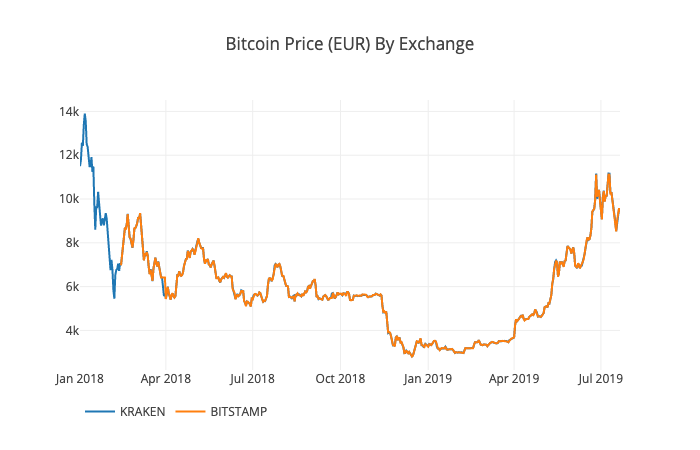
\includegraphics{5.png}
\end{figure}    
    
    We can now calculate a new column containing the average daily Bitcoin
price across all of the exchanges.

    \begin{Verbatim}[commandchars=\\\{\}]
{\color{incolor}In [{\color{incolor}41}]:} \PY{n}{btc\PYZus{}eur\PYZus{}datasets}\PY{p}{[}\PY{l+s+s1}{\PYZsq{}}\PY{l+s+s1}{avg\PYZus{}btc\PYZus{}price\PYZus{}eur}\PY{l+s+s1}{\PYZsq{}}\PY{p}{]} \PY{o}{=} \PY{n}{btc\PYZus{}eur\PYZus{}datasets}\PY{o}{.}\PY{n}{mean}\PY{p}{(}\PY{n}{axis}\PY{o}{=}\PY{l+m+mi}{1}\PY{p}{)}
\end{Verbatim}

    \begin{Verbatim}[commandchars=\\\{\}]
{\color{incolor}In [{\color{incolor}42}]:} \PY{n}{btc\PYZus{}trace4} \PY{o}{=} \PY{n}{go}\PY{o}{.}\PY{n}{Scatter}\PY{p}{(}\PY{n}{x}\PY{o}{=}\PY{n}{btc\PYZus{}eur\PYZus{}datasets}\PY{o}{.}\PY{n}{index}\PY{p}{,}
                                \PY{n}{y}\PY{o}{=}\PY{n}{btc\PYZus{}eur\PYZus{}datasets}\PY{p}{[}\PY{l+s+s1}{\PYZsq{}}\PY{l+s+s1}{avg\PYZus{}btc\PYZus{}price\PYZus{}eur}\PY{l+s+s1}{\PYZsq{}}\PY{p}{]}\PY{p}{)}
\end{Verbatim}

    \begin{Verbatim}[commandchars=\\\{\}]
{\color{incolor}In [{\color{incolor}43}]:} \PY{n}{data} \PY{o}{=} \PY{p}{[}\PY{n}{btc\PYZus{}trace4}\PY{p}{]}
         \PY{n}{layout} \PY{o}{=} \PY{n+nb}{dict}\PY{p}{(}\PY{n}{title} \PY{o}{=} \PY{l+s+s1}{\PYZsq{}}\PY{l+s+s1}{Average Price}\PY{l+s+s1}{\PYZsq{}}\PY{p}{,} \PY{n}{xaxis} \PY{o}{=} \PY{n+nb}{dict}\PY{p}{(}\PY{n}{title} \PY{o}{=} \PY{l+s+s1}{\PYZsq{}}\PY{l+s+s1}{Date}\PY{l+s+s1}{\PYZsq{}}\PY{p}{)}\PY{p}{,}
                       \PY{n}{yaxis} \PY{o}{=} \PY{n+nb}{dict}\PY{p}{(}\PY{n}{title} \PY{o}{=} \PY{l+s+s1}{\PYZsq{}}\PY{l+s+s1}{Price, EUR}\PY{l+s+s1}{\PYZsq{}}\PY{p}{)}\PY{p}{)}
         \PY{n}{fig} \PY{o}{=} \PY{n+nb}{dict}\PY{p}{(}\PY{n}{data}\PY{o}{=}\PY{n}{data}\PY{p}{,} \PY{n}{layout}\PY{o}{=}\PY{n}{layout}\PY{p}{)}
         \PY{n}{plotly}\PY{o}{.}\PY{n}{offline}\PY{o}{.}\PY{n}{iplot}\PY{p}{(}\PY{n}{fig}\PY{p}{)}
\end{Verbatim}

\begin{figure}[H]
	\centering
		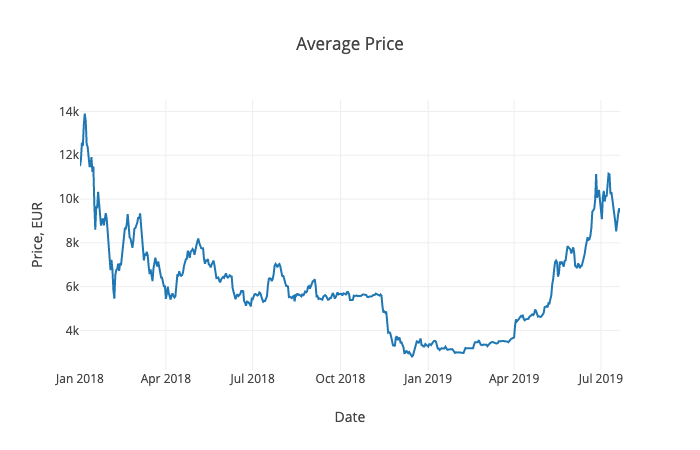
\includegraphics{6.png}
\end{figure}     
    
    This new column is our Bitcoin pricing index.

    Conclusions: In recent months we have witnessed an exponential growth of
Bitcoins. From 1 January 2017 to 1 January 2018, Bitcoin had a
percentage gain of 1418\%. Bitcoin's historic high was \$ 20089, reached
near the arrival of CBOE futures (Chicago Board Option Exchange) and CME
(Chicago Mercantile Exchange).

    The commercial use of Bitcoin, and in general of cryptocurrencies, in
the purchases of everyday life is profoundly influenced by volatility
since the purchase of an asset, and therefore the passage of money, must
guarantee a certain stability of value.

    \hypertarget{researching-the-model-that-will-be-best-for-the-type-of-data}{%
\section{Researching the model that will be best for the type of
data}\label{researching-the-model-that-will-be-best-for-the-type-of-data}}

    Our main goal is to train the best performing model possible, using the
pre-processed data.

    In Supervised learning, an AI system is presented with data which is
labelled, which means that each data tagged with the correct label. The
supervised learning is categorized into 2 other categories which are
``Classification'' and ``Regression''.

    \hypertarget{training-and-testing-the-model-on-data}{%
\section{Training and testing the model on
data}\label{training-and-testing-the-model-on-data}}

    In general for training a model we initially split the model into 3
three sections which are ``Training data'' ,``Validation data'' and
``Testing data''.

\begin{itemize}
\tightlist
\item
  Training set: The training set is the material through which the
  computer learns how to process information. Machine learning uses
  algorithms to perform the training part. A set of data used for
  learning, that is to fit the parameters of the classifier.
\item
  Validation set: Cross-validation is primarily used in applied machine
  learning to estimate the skill of a machine learning model on unseen
  data. A set of unseen data is used from the training data to tune the
  parameters of a classifier.
\item
  Test set: A set of unseen data used only to assess the performance of
  a fully-specified classifier.
\end{itemize}

    Once the data is divided into the 3 given segments we can start the
training process. In our case we only use train and test for LSTM and
ARIMA models.

\begin{figure}[H]
	\centering
		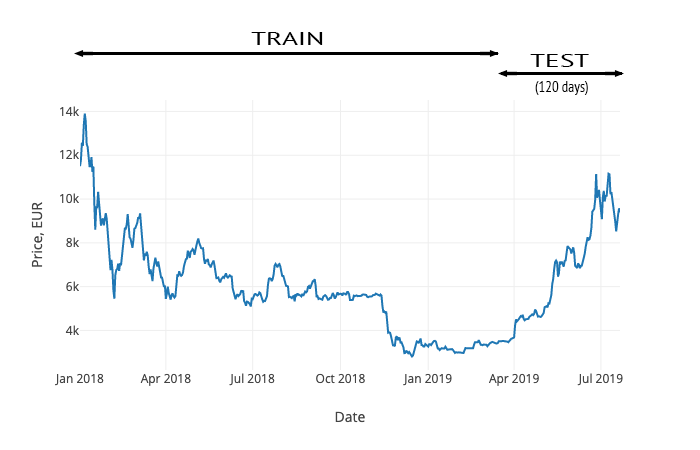
\includegraphics{traintest.png}
		  \caption{Figure 2 : Train and Test model}
\end{figure} 

    \hypertarget{lstm}{%
\section{LSTM}\label{lstm}}

    Since we are using a time series dataset, it is not viable to use a
feedforward-only neural network as tomorrow's BTC price is most
correlated with today's, not a month ago's.

A recurrent neural network (RNN) is a class of artificial neural network
where connections between nodes form a directed graph along a sequence.
An RNN shows temporal dynamic behavior for a time sequence and it can
use its internal state to process sequences.

    Time series forecasting is quite different from other machine learning
models because: 1. It is time dependent. 2. Along with an increasing or
decreasing trend, most time series have some form of seasonality trends,
i.e.~variations specific to a particular time frame.

    \textbf{Long Short Term Memory networks (LSTM)} are a special kind of
RNN (Recurrent Neural Network) capable of learning long-term
dependencies. They were introduced by Hochreiter \& Schmidhuber (1997)
and were refined and popularized by many people in following work. They
work tremendously well on a large variety of problems, and are now
widely used.

    LSTMs are explicitly designed to avoid the long-term dependency problem.
Remembering information for long periods of time is practically their
default behavior.

\begin{figure}[H]
	\centering
		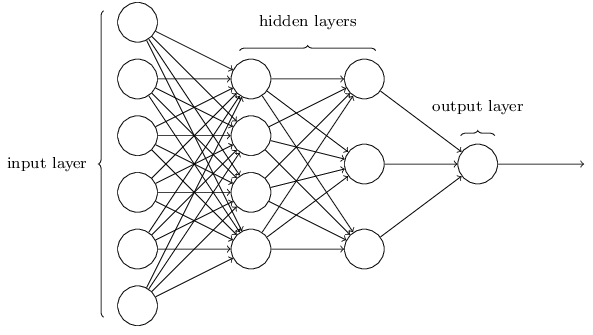
\includegraphics{nn.png}
		  \caption{Figure 3 : Neural Network (NN)}
\end{figure} 
    
\begin{figure}[H]
	\centering
		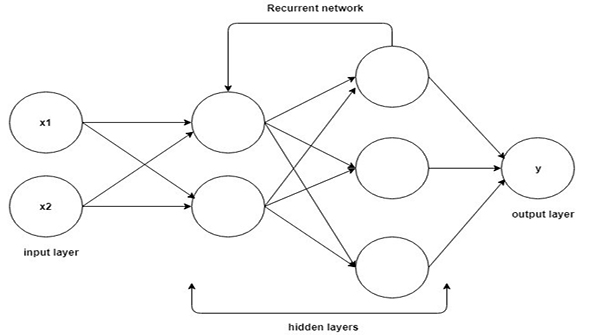
\includegraphics{rnn.jpeg}
		  \caption{Figure 4 : Recurrent Neural Network (RNN)}
\end{figure} 


    We begin to import our original dataset and defining it as \emph{data}:

    \begin{Verbatim}[commandchars=\\\{\}]
{\color{incolor}In [{\color{incolor}44}]:} \PY{n}{data} \PY{o}{=} \PY{n}{btc\PYZus{}eur\PYZus{}price\PYZus{}kraken}
\end{Verbatim}

    We Use MinMaxScaler, estimator scales and translates each feature
individually such that it is in the given range on the training set to
normalize \emph{Weighted Price} to range from \(0\) to \(1\):

    \begin{Verbatim}[commandchars=\\\{\}]
{\color{incolor}In [{\color{incolor}45}]:} \PY{n}{values} \PY{o}{=} \PY{n}{data}\PY{p}{[}\PY{l+s+s1}{\PYZsq{}}\PY{l+s+s1}{Weighted Price}\PY{l+s+s1}{\PYZsq{}}\PY{p}{]}\PY{o}{.}\PY{n}{values}\PY{o}{.}\PY{n}{reshape}\PY{p}{(}\PY{o}{\PYZhy{}}\PY{l+m+mi}{1}\PY{p}{,}\PY{l+m+mi}{1}\PY{p}{)}
         \PY{n}{values} \PY{o}{=} \PY{n}{values}\PY{o}{.}\PY{n}{astype}\PY{p}{(}\PY{l+s+s1}{\PYZsq{}}\PY{l+s+s1}{float32}\PY{l+s+s1}{\PYZsq{}}\PY{p}{)}
         \PY{n}{scaler} \PY{o}{=} \PY{n}{MinMaxScaler}\PY{p}{(}\PY{n}{feature\PYZus{}range}\PY{o}{=}\PY{p}{(}\PY{l+m+mi}{0}\PY{p}{,} \PY{l+m+mi}{1}\PY{p}{)}\PY{p}{)}
         \PY{n}{scaled} \PY{o}{=} \PY{n}{scaler}\PY{o}{.}\PY{n}{fit\PYZus{}transform}\PY{p}{(}\PY{n}{values}\PY{p}{)}
\end{Verbatim}

    Data scaling or normalization is a process of making model data in a
standard format so that the training is improved, accurate, and faster.
The method of scaling data in neural networks is similar to data
normalization in any machine learning problem.

    A Machine Learning algorithm needs to be trained on a set of data to
learn the relationships between different features and how these
features affect the target variable. For this we need to divide the
entire data set into two sets. One is the training set on which we are
going to train our algorithm to build a model. The other is the testing
set on which we will test our model to see how accurate its predictions
are.

    We want to predict the BTC price for three month, so we take the data of
last 120 days as the test set.

    \begin{Verbatim}[commandchars=\\\{\}]
{\color{incolor}In [{\color{incolor}46}]:} \PY{n}{prediction\PYZus{}days} \PY{o}{=} \PY{l+m+mi}{120}
         \PY{n}{train}\PY{o}{=} \PY{n}{scaled}\PY{p}{[}\PY{p}{:}\PY{n+nb}{len}\PY{p}{(}\PY{n}{scaled}\PY{p}{)} \PY{o}{\PYZhy{}} \PY{n}{prediction\PYZus{}days}\PY{p}{]}
         \PY{n}{test}\PY{o}{=} \PY{n}{scaled}\PY{p}{[}\PY{n+nb}{len}\PY{p}{(}\PY{n}{scaled}\PY{p}{)} \PY{o}{\PYZhy{}} \PY{n}{prediction\PYZus{}days}\PY{p}{:}\PY{p}{]}
         \PY{n+nb}{print}\PY{p}{(}\PY{n+nb}{len}\PY{p}{(}\PY{n}{train}\PY{p}{)}\PY{p}{,} \PY{n+nb}{len}\PY{p}{(}\PY{n}{test}\PY{p}{)}\PY{p}{)}
\end{Verbatim}

    \begin{Verbatim}[commandchars=\\\{\}]
447 120

    \end{Verbatim}

    In the next cell we define a function which creates \emph{X} inputs and
\emph{Y} labels for our model. In the sequential forecasting, we predict
the future value based on some previous and current values. So, our
\emph{Y} label is the value from the next (future) point of time while
the \emph{X} inputs are one or several values from the past.

\begin{figure}[H]
	\centering
		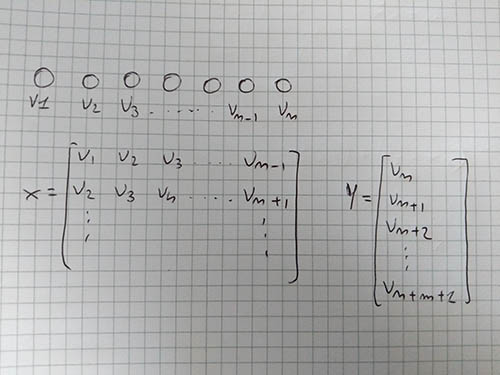
\includegraphics{xy.png}
\end{figure} 

    The amount of these values we can set by tuning the parameter
\emph{look\_back} in our function. If we set it to \emph{1}, this means
that we predict current value \emph{t} based on the previous value
\emph{(t-1)}. The value \emph{t} corresponds to the current day.

    \begin{Verbatim}[commandchars=\\\{\}]
{\color{incolor}In [{\color{incolor}47}]:} \PY{k}{def} \PY{n+nf}{create\PYZus{}dataset}\PY{p}{(}\PY{n}{dataset}\PY{p}{,} \PY{n}{look\PYZus{}back}\PY{o}{=}\PY{l+m+mi}{1}\PY{p}{)}\PY{p}{:}
             \PY{n}{dataX}\PY{p}{,} \PY{n}{dataY} \PY{o}{=} \PY{p}{[}\PY{p}{]}\PY{p}{,} \PY{p}{[}\PY{p}{]}
             \PY{k}{for} \PY{n}{i} \PY{o+ow}{in} \PY{n+nb}{range}\PY{p}{(}\PY{n+nb}{len}\PY{p}{(}\PY{n}{dataset}\PY{p}{)} \PY{o}{\PYZhy{}} \PY{n}{look\PYZus{}back}\PY{p}{)}\PY{p}{:}
                 \PY{n}{a} \PY{o}{=} \PY{n}{dataset}\PY{p}{[}\PY{n}{i}\PY{p}{:}\PY{p}{(}\PY{n}{i} \PY{o}{+} \PY{n}{look\PYZus{}back}\PY{p}{)}\PY{p}{,} \PY{l+m+mi}{0}\PY{p}{]}
                 \PY{n}{dataX}\PY{o}{.}\PY{n}{append}\PY{p}{(}\PY{n}{a}\PY{p}{)}
                 \PY{n}{dataY}\PY{o}{.}\PY{n}{append}\PY{p}{(}\PY{n}{dataset}\PY{p}{[}\PY{n}{i} \PY{o}{+} \PY{n}{look\PYZus{}back}\PY{p}{,} \PY{l+m+mi}{0}\PY{p}{]}\PY{p}{)}
             \PY{n+nb}{print}\PY{p}{(}\PY{n+nb}{len}\PY{p}{(}\PY{n}{dataY}\PY{p}{)}\PY{p}{)}
             \PY{k}{return} \PY{n}{np}\PY{o}{.}\PY{n}{array}\PY{p}{(}\PY{n}{dataX}\PY{p}{)}\PY{p}{,} \PY{n}{np}\PY{o}{.}\PY{n}{array}\PY{p}{(}\PY{n}{dataY}\PY{p}{)}
\end{Verbatim}

    We generate dataset for \emph{trainX}, \emph{trainY}, \emph{testX},
\emph{testY} and reshape \emph{X} for model training to give a new shape
without changing the data:

    \begin{Verbatim}[commandchars=\\\{\}]
{\color{incolor}In [{\color{incolor}48}]:} \PY{n}{look\PYZus{}back} \PY{o}{=} \PY{l+m+mi}{1}
         \PY{n}{trainX}\PY{p}{,} \PY{n}{trainY} \PY{o}{=} \PY{n}{create\PYZus{}dataset}\PY{p}{(}\PY{n}{train}\PY{p}{,} \PY{n}{look\PYZus{}back}\PY{p}{)}
         \PY{n}{testX}\PY{p}{,} \PY{n}{testY} \PY{o}{=} \PY{n}{create\PYZus{}dataset}\PY{p}{(}\PY{n}{test}\PY{p}{,} \PY{n}{look\PYZus{}back}\PY{p}{)}
\end{Verbatim}

    \begin{Verbatim}[commandchars=\\\{\}]
446
119

    \end{Verbatim}

    \begin{Verbatim}[commandchars=\\\{\}]
{\color{incolor}In [{\color{incolor}49}]:} \PY{n}{trainX} \PY{o}{=} \PY{n}{np}\PY{o}{.}\PY{n}{reshape}\PY{p}{(}\PY{n}{trainX}\PY{p}{,} \PY{p}{(}\PY{n}{trainX}\PY{o}{.}\PY{n}{shape}\PY{p}{[}\PY{l+m+mi}{0}\PY{p}{]}\PY{p}{,} \PY{l+m+mi}{1}\PY{p}{,} \PY{n}{trainX}\PY{o}{.}\PY{n}{shape}\PY{p}{[}\PY{l+m+mi}{1}\PY{p}{]}\PY{p}{)}\PY{p}{)}
         \PY{n}{testX} \PY{o}{=} \PY{n}{np}\PY{o}{.}\PY{n}{reshape}\PY{p}{(}\PY{n}{testX}\PY{p}{,} \PY{p}{(}\PY{n}{testX}\PY{o}{.}\PY{n}{shape}\PY{p}{[}\PY{l+m+mi}{0}\PY{p}{]}\PY{p}{,} \PY{l+m+mi}{1}\PY{p}{,} \PY{n}{testX}\PY{o}{.}\PY{n}{shape}\PY{p}{[}\PY{l+m+mi}{1}\PY{p}{]}\PY{p}{)}\PY{p}{)}
\end{Verbatim}

    Eventually, we can build and train our model.

    The LSTM model that we are going to create will be a sequential model
with multiple layers.

    We imported the Sequential class from keras.models library and LSTM and
Dense classes from keras.layers library.

    The first parameter to the LSTM layer is the number of neurons or nodes
that we want in the layer.

    Dropout layer is added to avoid overfitting, which is a phenomenon where
a machine learning model performs better on the training data compared
to the test data.

    To make our model more robust we add a dense layer at the end of the
model. The number of neurons in the dense layer will be set to 1 since
we want to predict a single value in the output.

    We call the compile method on the Sequential model object which is
``model'' in our case. We use the mean squared error as loss function
and to reduce the loss or to optimize the algorithm, we use the adam
optimizer.

    \hypertarget{adam-algorithm}{%
\subsection{Adam Algorithm}\label{adam-algorithm}}

    Adam is an optimization algorithm that can used instead of the classical
stochastic gradient descent procedure to update network weights
iterative based in training data.

    The Adam optimization algorithm is a combination of the gradient descent
with momentum algorithm and the RMS (Root Mean Square) Prop algorithm.

    Adam is an optimization algorithm that can used instead of the classical
stochastic gradient descent procedure to update network weights
iterative based in training data.

The Adam optimization algorithm is a combination of the gradient descent
with momentum algorithm and the RMS (Root Mean Square) Prop algorithm.

There are several advantages of the Adam Algorithm and some of them are
listed below:

\begin{itemize}
\tightlist
\item
  Easy to implement
\item
  Quite computationally efficient
\item
  Requires little memory space
\item
  Good for non-stationary objectives
\item
  Works well on problems with noisy or sparse gradients
\item
  Works well with large data sets and large parameters
\end{itemize}

    Adam takes into account the moving average of the prime moments \(m\)
and the second \(v\) of the gradient using the correct estimators
\(hat{m}\) and \(hat{v}\) to contrast the bias towards \emph{0} in the
first iterations. Indicating the parameters with \(w_{t}\) for the
iteration \(t\) and with \(Q\) the cost function to optimize, we have:

\(m_{t+1}=\beta_{1}m_{t}+(1-\beta_{1})\nabla Q(w_{t})\)

\(v_{t+1}=\beta_{1}v_{t}+(1-\beta_{2})(\nabla Q(w_{t}))^2\)

\(\hat{m}=\frac{m_{t+1}}{1-\beta_{1}^{t+1}}\)

\(\hat{v}=\frac{v_{t+1}}{1-\beta_{2}^{t+1}}\)

\(w_{t+1}=w_{t}-\eta{\frac{\hat{m}}{{\sqrt{\hat{v}}}+\epsilon}}\)

where \(\epsilon\) is a smoothing term added for the purpose of
numerical stability, \(\beta_{1}\) and \(\beta_{2}\) are hyperparameters
that control exponential decay.

    IMPORTANT: We keep track of both the training and test loss during
training by setting the validation\_data argument in the fit() function.
At the end of the run both the training and test loss are plotted. We
don't need to use a validation data set, it's a choice.

    Now is the time to train the model that we defined in the previous few
steps. To do so we call the fit method on the model and pass it our
training features and labels as shown below:

    \begin{Verbatim}[commandchars=\\\{\}]
{\color{incolor}In [{\color{incolor}50}]:} \PY{n}{model} \PY{o}{=} \PY{n}{Sequential}\PY{p}{(}\PY{p}{)}
         \PY{n}{model}\PY{o}{.}\PY{n}{add}\PY{p}{(}\PY{n}{LSTM}\PY{p}{(}\PY{l+m+mi}{100}\PY{p}{,} \PY{n}{input\PYZus{}shape}\PY{o}{=}\PY{p}{(}\PY{n}{trainX}\PY{o}{.}\PY{n}{shape}\PY{p}{[}\PY{l+m+mi}{1}\PY{p}{]}\PY{p}{,} \PY{n}{trainX}\PY{o}{.}\PY{n}{shape}\PY{p}{[}\PY{l+m+mi}{2}\PY{p}{]}\PY{p}{)}\PY{p}{)}\PY{p}{)}
         \PY{n}{model}\PY{o}{.}\PY{n}{add}\PY{p}{(}\PY{n}{Dropout}\PY{p}{(}\PY{l+m+mf}{0.2}\PY{p}{)}\PY{p}{)}
         \PY{n}{model}\PY{o}{.}\PY{n}{add}\PY{p}{(}\PY{n}{Dense}\PY{p}{(}\PY{l+m+mi}{1}\PY{p}{)}\PY{p}{)}
         \PY{n}{model}\PY{o}{.}\PY{n}{compile}\PY{p}{(}\PY{n}{loss}\PY{o}{=}\PY{l+s+s1}{\PYZsq{}}\PY{l+s+s1}{mse}\PY{l+s+s1}{\PYZsq{}}\PY{p}{,} \PY{n}{optimizer}\PY{o}{=}\PY{l+s+s1}{\PYZsq{}}\PY{l+s+s1}{adam}\PY{l+s+s1}{\PYZsq{}}\PY{p}{)}
         \PY{n}{history} \PY{o}{=} \PY{n}{model}\PY{o}{.}\PY{n}{fit}\PY{p}{(}\PY{n}{trainX}\PY{p}{,} \PY{n}{trainY}\PY{p}{,} 
                                         \PY{n}{epochs}\PY{o}{=}\PY{l+m+mi}{1000}\PY{p}{,} \PY{n}{batch\PYZus{}size}\PY{o}{=}\PY{l+m+mi}{200}\PY{p}{,} 
                                         \PY{n}{validation\PYZus{}data}\PY{o}{=}\PY{p}{(}\PY{n}{testX}\PY{p}{,} \PY{n}{testY}\PY{p}{)}\PY{p}{,} 
                                         \PY{n}{verbose}\PY{o}{=}\PY{l+m+mi}{0}\PY{p}{,} \PY{n}{shuffle}\PY{o}{=}\PY{k+kc}{False}\PY{p}{)}
\end{Verbatim}

    \begin{Verbatim}[commandchars=\\\{\}]
WARNING:tensorflow:From /Library/Frameworks/Python.framework/Versions/3.7/lib/python3.7/site-packages/tensorflow/python/framework/op\_def\_library.py:263: colocate\_with (from tensorflow.python.framework.ops) is deprecated and will be removed in a future version.
Instructions for updating:
Colocations handled automatically by placer.

    \end{Verbatim}

    \begin{Verbatim}[commandchars=\\\{\}]
WARNING:tensorflow:From /Library/Frameworks/Python.framework/Versions/3.7/lib/python3.7/site-packages/tensorflow/python/framework/op\_def\_library.py:263: colocate\_with (from tensorflow.python.framework.ops) is deprecated and will be removed in a future version.
Instructions for updating:
Colocations handled automatically by placer.

    \end{Verbatim}

    \begin{Verbatim}[commandchars=\\\{\}]
WARNING:tensorflow:From /Library/Frameworks/Python.framework/Versions/3.7/lib/python3.7/site-packages/keras/backend/tensorflow\_backend.py:3445: calling dropout (from tensorflow.python.ops.nn\_ops) with keep\_prob is deprecated and will be removed in a future version.
Instructions for updating:
Please use `rate` instead of `keep\_prob`. Rate should be set to `rate = 1 - keep\_prob`.

    \end{Verbatim}

    \begin{Verbatim}[commandchars=\\\{\}]
WARNING:tensorflow:From /Library/Frameworks/Python.framework/Versions/3.7/lib/python3.7/site-packages/keras/backend/tensorflow\_backend.py:3445: calling dropout (from tensorflow.python.ops.nn\_ops) with keep\_prob is deprecated and will be removed in a future version.
Instructions for updating:
Please use `rate` instead of `keep\_prob`. Rate should be set to `rate = 1 - keep\_prob`.

    \end{Verbatim}

    \begin{Verbatim}[commandchars=\\\{\}]
WARNING:tensorflow:From /Library/Frameworks/Python.framework/Versions/3.7/lib/python3.7/site-packages/tensorflow/python/ops/math\_ops.py:3066: to\_int32 (from tensorflow.python.ops.math\_ops) is deprecated and will be removed in a future version.
Instructions for updating:
Use tf.cast instead.

    \end{Verbatim}

    \begin{Verbatim}[commandchars=\\\{\}]
WARNING:tensorflow:From /Library/Frameworks/Python.framework/Versions/3.7/lib/python3.7/site-packages/tensorflow/python/ops/math\_ops.py:3066: to\_int32 (from tensorflow.python.ops.math\_ops) is deprecated and will be removed in a future version.
Instructions for updating:
Use tf.cast instead.

    \end{Verbatim}

    We have trained our model.

    On the plot below we compare the Train and Test loss on each iteration
of the training process. We can see, that after some iterations the
train and test loss became very similar, which is a good sign (this
means we are not overfitting the train set).

    \begin{Verbatim}[commandchars=\\\{\}]
{\color{incolor}In [{\color{incolor}51}]:} \PY{n}{pyplot}\PY{o}{.}\PY{n}{plot}\PY{p}{(}\PY{n}{history}\PY{o}{.}\PY{n}{history}\PY{p}{[}\PY{l+s+s1}{\PYZsq{}}\PY{l+s+s1}{loss}\PY{l+s+s1}{\PYZsq{}}\PY{p}{]}\PY{p}{,} \PY{n}{label}\PY{o}{=}\PY{l+s+s1}{\PYZsq{}}\PY{l+s+s1}{train}\PY{l+s+s1}{\PYZsq{}}\PY{p}{)}
         \PY{n}{pyplot}\PY{o}{.}\PY{n}{plot}\PY{p}{(}\PY{n}{history}\PY{o}{.}\PY{n}{history}\PY{p}{[}\PY{l+s+s1}{\PYZsq{}}\PY{l+s+s1}{val\PYZus{}loss}\PY{l+s+s1}{\PYZsq{}}\PY{p}{]}\PY{p}{,} \PY{n}{label}\PY{o}{=}\PY{l+s+s1}{\PYZsq{}}\PY{l+s+s1}{test}\PY{l+s+s1}{\PYZsq{}}\PY{p}{)}
         \PY{n}{pyplot}\PY{o}{.}\PY{n}{legend}\PY{p}{(}\PY{p}{)}
         \PY{n}{pyplot}\PY{o}{.}\PY{n}{show}\PY{p}{(}\PY{p}{)}
\end{Verbatim}

    \begin{center}
    \adjustimage{max size={0.9\linewidth}{0.9\paperheight}}{output_147_0.png}
    \end{center}
    { \hspace*{\fill} \\}
    
    We make prediction using \emph{textX} and plotting line graph against
\emph{testY}.

    \begin{Verbatim}[commandchars=\\\{\}]
{\color{incolor}In [{\color{incolor}52}]:} \PY{n}{yhat} \PY{o}{=} \PY{n}{model}\PY{o}{.}\PY{n}{predict}\PY{p}{(}\PY{n}{testX}\PY{p}{)}
         \PY{n}{pyplot}\PY{o}{.}\PY{n}{plot}\PY{p}{(}\PY{n}{yhat}\PY{p}{,} \PY{n}{label}\PY{o}{=}\PY{l+s+s1}{\PYZsq{}}\PY{l+s+s1}{predict}\PY{l+s+s1}{\PYZsq{}}\PY{p}{)}
         \PY{n}{pyplot}\PY{o}{.}\PY{n}{plot}\PY{p}{(}\PY{n}{testY}\PY{p}{,} \PY{n}{label}\PY{o}{=}\PY{l+s+s1}{\PYZsq{}}\PY{l+s+s1}{true}\PY{l+s+s1}{\PYZsq{}}\PY{p}{)}
         \PY{n}{pyplot}\PY{o}{.}\PY{n}{legend}\PY{p}{(}\PY{p}{)}
         \PY{n}{pyplot}\PY{o}{.}\PY{n}{show}\PY{p}{(}\PY{p}{)}
\end{Verbatim}

    \begin{center}
    \adjustimage{max size={0.9\linewidth}{0.9\paperheight}}{output_149_0.png}
    \end{center}
    { \hspace*{\fill} \\}
    
    We scaler Inverse \emph{Y} back to normal value:

    \begin{Verbatim}[commandchars=\\\{\}]
{\color{incolor}In [{\color{incolor}53}]:} \PY{n}{yhat\PYZus{}inverse} \PY{o}{=} \PY{n}{scaler}\PY{o}{.}\PY{n}{inverse\PYZus{}transform}\PY{p}{(}\PY{n}{yhat}\PY{o}{.}\PY{n}{reshape}\PY{p}{(}\PY{o}{\PYZhy{}}\PY{l+m+mi}{1}\PY{p}{,} \PY{l+m+mi}{1}\PY{p}{)}\PY{p}{)}
         \PY{n}{testY\PYZus{}inverse} \PY{o}{=} \PY{n}{scaler}\PY{o}{.}\PY{n}{inverse\PYZus{}transform}\PY{p}{(}\PY{n}{testY}\PY{o}{.}\PY{n}{reshape}\PY{p}{(}\PY{o}{\PYZhy{}}\PY{l+m+mi}{1}\PY{p}{,} \PY{l+m+mi}{1}\PY{p}{)}\PY{p}{)}
\end{Verbatim}

    Evaluating the model accuracy is an essential part of the process in
creating machine learning models to describe how well the model is
performing in its predictions.

    We calculate the MSE, MAE and RMSE metrics, mainly used to evaluate the
prediction error rates and model performance in regression analysis:

    \begin{itemize}
\tightlist
\item
  \textbf{MAE (Mean Absolute Error)} : represents the difference between
  the original and predicted values extracted by averaged the absolute
  difference over the data set
\end{itemize}

    \begin{itemize}
\tightlist
\item
  \textbf{MSE (Mean Squared Error)} : represents the difference between
  the original and predicted values extracted by squared the average
  difference over the data set
\end{itemize}

    \begin{itemize}
\tightlist
\item
  \textbf{RMSE (Root Mean Squared Error)} : is the error rate by the
  square root of MSE
\end{itemize}

RMSE is an intuitive estimator of the quality of the model.

    \begin{Verbatim}[commandchars=\\\{\}]
{\color{incolor}In [{\color{incolor}54}]:} \PY{n}{mae} \PY{o}{=} \PY{n}{mean\PYZus{}absolute\PYZus{}error}\PY{p}{(}\PY{n}{testY\PYZus{}inverse}\PY{p}{,} \PY{n}{yhat\PYZus{}inverse}\PY{p}{)}
         \PY{n+nb}{print}\PY{p}{(}\PY{l+s+s1}{\PYZsq{}}\PY{l+s+s1}{MAE: }\PY{l+s+si}{\PYZpc{}.3f}\PY{l+s+s1}{\PYZsq{}} \PY{o}{\PYZpc{}} \PY{n}{mae}\PY{p}{)}
         \PY{n}{mse} \PY{o}{=} \PY{n}{mean\PYZus{}squared\PYZus{}error}\PY{p}{(}\PY{n}{testY\PYZus{}inverse}\PY{p}{,} \PY{n}{yhat\PYZus{}inverse}\PY{p}{)}
         \PY{n+nb}{print}\PY{p}{(}\PY{l+s+s1}{\PYZsq{}}\PY{l+s+s1}{MSE: }\PY{l+s+si}{\PYZpc{}.3f}\PY{l+s+s1}{\PYZsq{}} \PY{o}{\PYZpc{}} \PY{n}{mse}\PY{p}{)}
         \PY{n}{rmse} \PY{o}{=} \PY{n}{sqrt}\PY{p}{(}\PY{n}{mse}\PY{p}{)}
         \PY{n+nb}{print}\PY{p}{(}\PY{l+s+s1}{\PYZsq{}}\PY{l+s+s1}{RMSE: }\PY{l+s+si}{\PYZpc{}.3f}\PY{l+s+s1}{\PYZsq{}} \PY{o}{\PYZpc{}} \PY{n}{rmse}\PY{p}{)}
\end{Verbatim}

    \begin{Verbatim}[commandchars=\\\{\}]
MAE: 216.265
MSE: 103660.195
RMSE: 321.963

    \end{Verbatim}

    We plot line graph with \emph{Y} as \emph{EUR}.

    \begin{Verbatim}[commandchars=\\\{\}]
{\color{incolor}In [{\color{incolor}55}]:} \PY{n}{pyplot}\PY{o}{.}\PY{n}{plot}\PY{p}{(}\PY{n}{yhat\PYZus{}inverse}\PY{p}{,} \PY{n}{label}\PY{o}{=}\PY{l+s+s1}{\PYZsq{}}\PY{l+s+s1}{predict}\PY{l+s+s1}{\PYZsq{}}\PY{p}{)}
         \PY{n}{pyplot}\PY{o}{.}\PY{n}{plot}\PY{p}{(}\PY{n}{testY\PYZus{}inverse}\PY{p}{,} \PY{n}{label}\PY{o}{=}\PY{l+s+s1}{\PYZsq{}}\PY{l+s+s1}{actual}\PY{l+s+s1}{\PYZsq{}}\PY{p}{)}
         \PY{n}{pyplot}\PY{o}{.}\PY{n}{legend}\PY{p}{(}\PY{p}{)}
         \PY{n}{pyplot}\PY{o}{.}\PY{n}{show}\PY{p}{(}\PY{p}{)}
\end{Verbatim}

    \begin{center}
    \adjustimage{max size={0.9\linewidth}{0.9\paperheight}}{output_159_0.png}
    \end{center}
    { \hspace*{\fill} \\}
    
    We convert \emph{X} to dates and reshape \emph{testY} and \emph{yhat}
for plotly.

    \begin{Verbatim}[commandchars=\\\{\}]
{\color{incolor}In [{\color{incolor}56}]:} \PY{n}{predictDates} \PY{o}{=} \PY{n}{data}\PY{o}{.}\PY{n}{tail}\PY{p}{(}\PY{n+nb}{len}\PY{p}{(}\PY{n}{testX}\PY{p}{)}\PY{p}{)}\PY{o}{.}\PY{n}{index}
\end{Verbatim}

    \begin{Verbatim}[commandchars=\\\{\}]
{\color{incolor}In [{\color{incolor}57}]:} \PY{n}{testY\PYZus{}reshape} \PY{o}{=} \PY{n}{testY\PYZus{}inverse}\PY{o}{.}\PY{n}{reshape}\PY{p}{(}\PY{n+nb}{len}\PY{p}{(}\PY{n}{testY\PYZus{}inverse}\PY{p}{)}\PY{p}{)}
         \PY{n}{yhat\PYZus{}reshape} \PY{o}{=} \PY{n}{yhat\PYZus{}inverse}\PY{o}{.}\PY{n}{reshape}\PY{p}{(}\PY{n+nb}{len}\PY{p}{(}\PY{n}{yhat\PYZus{}inverse}\PY{p}{)}\PY{p}{)}
\end{Verbatim}

    We plot predicted and actual line graph with \emph{X=dates},
\emph{Y=EUR}:

    \begin{Verbatim}[commandchars=\\\{\}]
{\color{incolor}In [{\color{incolor}58}]:} \PY{n}{actual\PYZus{}chart} \PY{o}{=} \PY{n}{go}\PY{o}{.}\PY{n}{Scatter}\PY{p}{(}\PY{n}{x}\PY{o}{=}\PY{n}{predictDates}\PY{p}{,} \PY{n}{y}\PY{o}{=}\PY{n}{testY\PYZus{}reshape}\PY{p}{,} \PY{n}{name}\PY{o}{=} \PY{l+s+s1}{\PYZsq{}}\PY{l+s+s1}{Actual Price}\PY{l+s+s1}{\PYZsq{}}\PY{p}{)}
         \PY{n}{predict\PYZus{}chart} \PY{o}{=} \PY{n}{go}\PY{o}{.}\PY{n}{Scatter}\PY{p}{(}\PY{n}{x}\PY{o}{=}\PY{n}{predictDates}\PY{p}{,} \PY{n}{y}\PY{o}{=}\PY{n}{yhat\PYZus{}reshape}\PY{p}{,} \PY{n}{name}\PY{o}{=} \PY{l+s+s1}{\PYZsq{}}\PY{l+s+s1}{Predict Price}\PY{l+s+s1}{\PYZsq{}}\PY{p}{)}
         \PY{n}{plotly}\PY{o}{.}\PY{n}{offline}\PY{o}{.}\PY{n}{iplot}\PY{p}{(}\PY{p}{[}\PY{n}{predict\PYZus{}chart}\PY{p}{,} \PY{n}{actual\PYZus{}chart}\PY{p}{]}\PY{p}{)}
\end{Verbatim}

\begin{figure}[H]
	\centering
		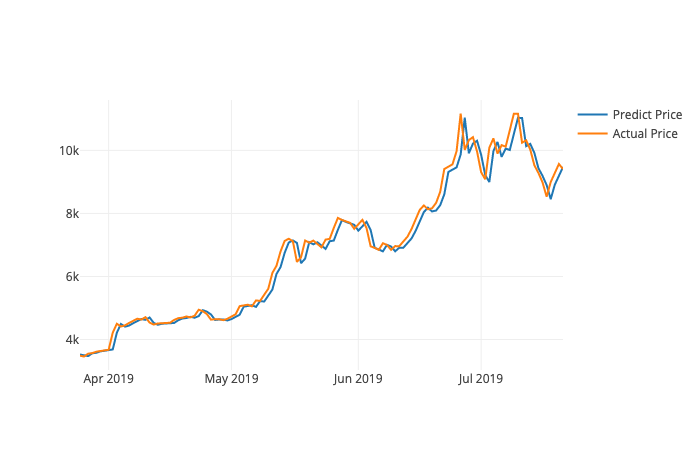
\includegraphics{7.png}
\end{figure}     
    
    Let's calculate a symmetric mean absolute percentage error (SMAPE). It
will show how good our predictions are in percentage. We define function
\emph{symmetric\_mean\_absolute\_percentage\_error} which will perform
all necessary calculations:

\(SMAPE=\frac {100\%}{n}\sum_{t=1}^{n}{\frac{\left|F_{t}-A_{t}\right|}{(|A_{t}|+|F_{t}|)/2}}\)

where \(F_t\) is the forecast value and \(A_t\) is the actual value.

    \begin{Verbatim}[commandchars=\\\{\}]
{\color{incolor}In [{\color{incolor}59}]:} \PY{k}{def} \PY{n+nf}{symmetric\PYZus{}mean\PYZus{}absolute\PYZus{}percentage\PYZus{}error}\PY{p}{(}\PY{n}{y\PYZus{}true}\PY{p}{,} \PY{n}{y\PYZus{}pred}\PY{p}{)}\PY{p}{:}
             \PY{k}{return} \PY{n}{np}\PY{o}{.}\PY{n}{mean}\PY{p}{(}\PY{n}{np}\PY{o}{.}\PY{n}{abs}\PY{p}{(}\PY{n}{y\PYZus{}pred} \PY{o}{\PYZhy{}} \PY{n}{y\PYZus{}true}\PY{p}{)} \PY{o}{/} \PY{p}{(}\PY{p}{(}\PY{n}{np}\PY{o}{.}\PY{n}{abs}\PY{p}{(}\PY{n}{y\PYZus{}true}\PY{p}{)} \PY{o}{+} \PY{n}{np}\PY{o}{.}\PY{n}{abs}\PY{p}{(}\PY{n}{y\PYZus{}pred}\PY{p}{)}\PY{p}{)}\PY{o}{/}\PY{l+m+mi}{2}\PY{p}{)}\PY{p}{)} \PY{o}{*} \PY{l+m+mi}{100}
         
         \PY{n}{SMAPE} \PY{o}{=} \PY{n}{symmetric\PYZus{}mean\PYZus{}absolute\PYZus{}percentage\PYZus{}error}\PY{p}{(}\PY{n}{testY\PYZus{}inverse}\PY{p}{,} \PY{n}{yhat\PYZus{}inverse}\PY{p}{)}
         
         \PY{n+nb}{print}\PY{p}{(}\PY{l+s+s1}{\PYZsq{}}\PY{l+s+s1}{Test SMAPE (percentage): }\PY{l+s+si}{\PYZpc{}.3f}\PY{l+s+s1}{\PYZsq{}} \PY{o}{\PYZpc{}} \PY{n}{SMAPE}\PY{p}{)}
\end{Verbatim}

    \begin{Verbatim}[commandchars=\\\{\}]
Test SMAPE (percentage): 2.869

    \end{Verbatim}

    \hypertarget{using-additional-features-for-model-training}{%
\subsection{Using additional features for model
training}\label{using-additional-features-for-model-training}}

    As we have seen before in the correlation matrix of our original
dataset, \emph{Volume} is correlated to \emph{Weighted Price}. Let's go
and work on this data.

    Machine learning methods like deep learning can be used for time series
forecasting. Before machine learning can be used, time series
forecasting problems must be re-framed as supervised learning problems
from a sequence to pairs of input and output.

    A key function to help transform time series data into a supervised
learning problem is the Pandas \emph{shift()} function.

    Given a DataFrame, the \emph{shift()} function can be used to create
copies of columns that are pushed forward (rows of NaN values added to
the front) or pulled back (rows of NaN values added to the end).

    We define a function named \emph{series\_to\_supervised()} that takes a
univariate or multivariate time series and frames it as a supervised
learning dataset.

    The function takes four arguments:

\begin{itemize}
\tightlist
\item
  data: Sequence of observations as a list or 2D NumPy array (Required).
\item
  n\_in: Number of lag observations as input (X). Values may be between
  \emph{{[}1..len(data){]}} (Optional, defaults to 1).
\item
  n\_out: Number of observations as output (y). Values may be between
  \emph{{[}0..len(data)-1{]}} (Optional, defaults to 1).
\item
  dropnan: Boolean whether or not to drop rows with NaN values
  (Optional, defaults to True).
\end{itemize}

The function returns a single value:

\begin{itemize}
\tightlist
\item
  return: Pandas DataFrame of series framed for supervised learning.
\end{itemize}

    The function to convert the series into supervised learning is this:

    \begin{Verbatim}[commandchars=\\\{\}]
{\color{incolor}In [{\color{incolor}60}]:} \PY{k}{def} \PY{n+nf}{series\PYZus{}to\PYZus{}supervised}\PY{p}{(}\PY{n}{data}\PY{p}{,} \PY{n}{n\PYZus{}in}\PY{o}{=}\PY{l+m+mi}{1}\PY{p}{,} \PY{n}{n\PYZus{}out}\PY{o}{=}\PY{l+m+mi}{1}\PY{p}{,} \PY{n}{dropnan}\PY{o}{=}\PY{k+kc}{True}\PY{p}{)}\PY{p}{:}
             \PY{n}{n\PYZus{}vars} \PY{o}{=} \PY{l+m+mi}{1} \PY{k}{if} \PY{n+nb}{type}\PY{p}{(}\PY{n}{data}\PY{p}{)} \PY{o+ow}{is} \PY{n+nb}{list} \PY{k}{else} \PY{n}{data}\PY{o}{.}\PY{n}{shape}\PY{p}{[}\PY{l+m+mi}{1}\PY{p}{]}
             \PY{n}{df} \PY{o}{=} \PY{n}{pd}\PY{o}{.}\PY{n}{DataFrame}\PY{p}{(}\PY{n}{data}\PY{p}{)}
             \PY{n}{cols}\PY{p}{,} \PY{n}{names} \PY{o}{=} \PY{n+nb}{list}\PY{p}{(}\PY{p}{)}\PY{p}{,} \PY{n+nb}{list}\PY{p}{(}\PY{p}{)}
         \PY{c+c1}{\PYZsh{} input sequence (t\PYZhy{}n, ... t\PYZhy{}1)}
             \PY{k}{for} \PY{n}{i} \PY{o+ow}{in} \PY{n+nb}{range}\PY{p}{(}\PY{n}{n\PYZus{}in}\PY{p}{,} \PY{l+m+mi}{0}\PY{p}{,} \PY{o}{\PYZhy{}}\PY{l+m+mi}{1}\PY{p}{)}\PY{p}{:}
                 \PY{n}{cols}\PY{o}{.}\PY{n}{append}\PY{p}{(}\PY{n}{df}\PY{o}{.}\PY{n}{shift}\PY{p}{(}\PY{n}{i}\PY{p}{)}\PY{p}{)}
                 \PY{n}{names} \PY{o}{+}\PY{o}{=} \PY{p}{[}\PY{p}{(}\PY{l+s+s1}{\PYZsq{}}\PY{l+s+s1}{var}\PY{l+s+si}{\PYZpc{}d}\PY{l+s+s1}{(t\PYZhy{}}\PY{l+s+si}{\PYZpc{}d}\PY{l+s+s1}{)}\PY{l+s+s1}{\PYZsq{}} \PY{o}{\PYZpc{}} \PY{p}{(}\PY{n}{j}\PY{o}{+}\PY{l+m+mi}{1}\PY{p}{,} \PY{n}{i}\PY{p}{)}\PY{p}{)} \PY{k}{for} \PY{n}{j} \PY{o+ow}{in} \PY{n+nb}{range}\PY{p}{(}\PY{n}{n\PYZus{}vars}\PY{p}{)}\PY{p}{]}
         \PY{c+c1}{\PYZsh{} forecast sequence (t, t+1, ... t+n)}
             \PY{k}{for} \PY{n}{i} \PY{o+ow}{in} \PY{n+nb}{range}\PY{p}{(}\PY{l+m+mi}{0}\PY{p}{,} \PY{n}{n\PYZus{}out}\PY{p}{)}\PY{p}{:}
                 \PY{n}{cols}\PY{o}{.}\PY{n}{append}\PY{p}{(}\PY{n}{df}\PY{o}{.}\PY{n}{shift}\PY{p}{(}\PY{o}{\PYZhy{}}\PY{n}{i}\PY{p}{)}\PY{p}{)}
                 \PY{k}{if} \PY{n}{i} \PY{o}{==} \PY{l+m+mi}{0}\PY{p}{:}
                     \PY{n}{names} \PY{o}{+}\PY{o}{=} \PY{p}{[}\PY{p}{(}\PY{l+s+s1}{\PYZsq{}}\PY{l+s+s1}{var}\PY{l+s+si}{\PYZpc{}d}\PY{l+s+s1}{(t)}\PY{l+s+s1}{\PYZsq{}} \PY{o}{\PYZpc{}} \PY{p}{(}\PY{n}{j}\PY{o}{+}\PY{l+m+mi}{1}\PY{p}{)}\PY{p}{)} \PY{k}{for} \PY{n}{j} \PY{o+ow}{in} \PY{n+nb}{range}\PY{p}{(}\PY{n}{n\PYZus{}vars}\PY{p}{)}\PY{p}{]}
                 \PY{k}{else}\PY{p}{:}
                     \PY{n}{names} \PY{o}{+}\PY{o}{=} \PY{p}{[}\PY{p}{(}\PY{l+s+s1}{\PYZsq{}}\PY{l+s+s1}{var}\PY{l+s+si}{\PYZpc{}d}\PY{l+s+s1}{(t+}\PY{l+s+si}{\PYZpc{}d}\PY{l+s+s1}{)}\PY{l+s+s1}{\PYZsq{}} \PY{o}{\PYZpc{}} \PY{p}{(}\PY{n}{j}\PY{o}{+}\PY{l+m+mi}{1}\PY{p}{,} \PY{n}{i}\PY{p}{)}\PY{p}{)} \PY{k}{for} \PY{n}{j} \PY{o+ow}{in} \PY{n+nb}{range}\PY{p}{(}\PY{n}{n\PYZus{}vars}\PY{p}{)}\PY{p}{]}
         \PY{c+c1}{\PYZsh{} put it all together}
             \PY{n}{agg} \PY{o}{=} \PY{n}{pd}\PY{o}{.}\PY{n}{concat}\PY{p}{(}\PY{n}{cols}\PY{p}{,} \PY{n}{axis}\PY{o}{=}\PY{l+m+mi}{1}\PY{p}{)}
             \PY{n}{agg}\PY{o}{.}\PY{n}{columns} \PY{o}{=} \PY{n}{names}
         \PY{c+c1}{\PYZsh{} drop rows with NaN values}
             \PY{k}{if} \PY{n}{dropnan}\PY{p}{:}
                 \PY{n}{agg}\PY{o}{.}\PY{n}{dropna}\PY{p}{(}\PY{n}{inplace}\PY{o}{=}\PY{k+kc}{True}\PY{p}{)}
             \PY{k}{return} \PY{n}{agg}
\end{Verbatim}

    We Get all data values, normalize features to range from \(0\) to \(1\)
and frame as supervised learning.

    \begin{Verbatim}[commandchars=\\\{\}]
{\color{incolor}In [{\color{incolor}61}]:} \PY{n}{values} \PY{o}{=} \PY{n}{data}\PY{p}{[}\PY{p}{[}\PY{l+s+s1}{\PYZsq{}}\PY{l+s+s1}{Weighted Price}\PY{l+s+s1}{\PYZsq{}}\PY{p}{]} 
                       \PY{o}{+} \PY{p}{[}\PY{l+s+s1}{\PYZsq{}}\PY{l+s+s1}{Volume (BTC)}\PY{l+s+s1}{\PYZsq{}}\PY{p}{]} \PY{o}{+} \PY{p}{[}\PY{l+s+s1}{\PYZsq{}}\PY{l+s+s1}{Volume (Currency)}\PY{l+s+s1}{\PYZsq{}}\PY{p}{]}\PY{p}{]}\PY{o}{.}\PY{n}{values}
         \PY{n}{values} \PY{o}{=} \PY{n}{values}\PY{o}{.}\PY{n}{astype}\PY{p}{(}\PY{l+s+s1}{\PYZsq{}}\PY{l+s+s1}{float32}\PY{l+s+s1}{\PYZsq{}}\PY{p}{)}
\end{Verbatim}

    \begin{Verbatim}[commandchars=\\\{\}]
{\color{incolor}In [{\color{incolor}62}]:} \PY{n}{scaler} \PY{o}{=} \PY{n}{MinMaxScaler}\PY{p}{(}\PY{n}{feature\PYZus{}range}\PY{o}{=}\PY{p}{(}\PY{l+m+mi}{0}\PY{p}{,} \PY{l+m+mi}{1}\PY{p}{)}\PY{p}{)}
         \PY{n}{scaled} \PY{o}{=} \PY{n}{scaler}\PY{o}{.}\PY{n}{fit\PYZus{}transform}\PY{p}{(}\PY{n}{values}\PY{p}{)}
\end{Verbatim}

    \begin{Verbatim}[commandchars=\\\{\}]
{\color{incolor}In [{\color{incolor}63}]:} \PY{n}{reframed} \PY{o}{=} \PY{n}{series\PYZus{}to\PYZus{}supervised}\PY{p}{(}\PY{n}{scaled}\PY{p}{,} \PY{l+m+mi}{1}\PY{p}{,} \PY{l+m+mi}{1}\PY{p}{)}
         \PY{n}{reframed}\PY{o}{.}\PY{n}{head}\PY{p}{(}\PY{p}{)}
\end{Verbatim}

\begin{Verbatim}[commandchars=\\\{\}]
{\color{outcolor}Out[{\color{outcolor}63}]:}    var1(t-1)  var2(t-1)  var3(t-1)   var1(t)   var2(t)   var3(t)
         1   0.782892   0.071342   0.150475  0.810345  0.132115  0.286039
         2   0.810345   0.132115   0.286039  0.879658  0.095292  0.219757
         3   0.879658   0.095292   0.219757  0.866885  0.113989  0.259912
         4   0.866885   0.113989   0.259912  0.953992  0.134293  0.330017
         5   0.953992   0.134293   0.330017  1.000000  0.080572  0.205544
\end{Verbatim}
            
    We drop unnecessary columns and split again data for training and
testing.

    \begin{Verbatim}[commandchars=\\\{\}]
{\color{incolor}In [{\color{incolor}64}]:} \PY{n}{reframed}\PY{o}{.}\PY{n}{drop}\PY{p}{(}\PY{n}{reframed}\PY{o}{.}\PY{n}{columns}\PY{p}{[}\PY{p}{[}\PY{l+m+mi}{4}\PY{p}{,}\PY{l+m+mi}{5}\PY{p}{]}\PY{p}{]}\PY{p}{,} \PY{n}{axis}\PY{o}{=}\PY{l+m+mi}{1}\PY{p}{,} \PY{n}{inplace}\PY{o}{=}\PY{k+kc}{True}\PY{p}{)}
         \PY{n+nb}{print}\PY{p}{(}\PY{n}{reframed}\PY{o}{.}\PY{n}{head}\PY{p}{(}\PY{p}{)}\PY{p}{)}
\end{Verbatim}

    \begin{Verbatim}[commandchars=\\\{\}]
   var1(t-1)  var2(t-1)  var3(t-1)   var1(t)
1   0.782892   0.071342   0.150475  0.810345
2   0.810345   0.132115   0.286039  0.879658
3   0.879658   0.095292   0.219757  0.866885
4   0.866885   0.113989   0.259912  0.953992
5   0.953992   0.134293   0.330017  1.000000

    \end{Verbatim}

    \begin{Verbatim}[commandchars=\\\{\}]
{\color{incolor}In [{\color{incolor}65}]:} \PY{n}{values} \PY{o}{=} \PY{n}{reframed}\PY{o}{.}\PY{n}{values}
         \PY{n}{n\PYZus{}train} \PY{o}{=} \PY{l+m+mi}{120}
         \PY{n}{train}\PY{o}{=} \PY{n}{values}\PY{p}{[}\PY{p}{:}\PY{n+nb}{len}\PY{p}{(}\PY{n}{values}\PY{p}{)} \PY{o}{\PYZhy{}} \PY{n}{n\PYZus{}train}\PY{p}{]}
         \PY{n}{test}\PY{o}{=} \PY{n}{values}\PY{p}{[}\PY{n+nb}{len}\PY{p}{(}\PY{n}{values}\PY{p}{)} \PY{o}{\PYZhy{}} \PY{n}{n\PYZus{}train}\PY{p}{:}\PY{p}{]}
         
         \PY{c+c1}{\PYZsh{} split into input and outputs}
         \PY{n}{train\PYZus{}X}\PY{p}{,} \PY{n}{train\PYZus{}y} \PY{o}{=} \PY{n}{train}\PY{p}{[}\PY{p}{:}\PY{p}{,} \PY{p}{:}\PY{o}{\PYZhy{}}\PY{l+m+mi}{1}\PY{p}{]}\PY{p}{,} \PY{n}{train}\PY{p}{[}\PY{p}{:}\PY{p}{,} \PY{o}{\PYZhy{}}\PY{l+m+mi}{1}\PY{p}{]}
         \PY{n}{test\PYZus{}X}\PY{p}{,} \PY{n}{test\PYZus{}y} \PY{o}{=} \PY{n}{test}\PY{p}{[}\PY{p}{:}\PY{p}{,} \PY{p}{:}\PY{o}{\PYZhy{}}\PY{l+m+mi}{1}\PY{p}{]}\PY{p}{,} \PY{n}{test}\PY{p}{[}\PY{p}{:}\PY{p}{,} \PY{o}{\PYZhy{}}\PY{l+m+mi}{1}\PY{p}{]}
         \PY{c+c1}{\PYZsh{} reshape input to be 3D}
         \PY{n}{train\PYZus{}X} \PY{o}{=} \PY{n}{train\PYZus{}X}\PY{o}{.}\PY{n}{reshape}\PY{p}{(}\PY{p}{(}\PY{n}{train\PYZus{}X}\PY{o}{.}\PY{n}{shape}\PY{p}{[}\PY{l+m+mi}{0}\PY{p}{]}\PY{p}{,} \PY{l+m+mi}{1}\PY{p}{,} \PY{n}{train\PYZus{}X}\PY{o}{.}\PY{n}{shape}\PY{p}{[}\PY{l+m+mi}{1}\PY{p}{]}\PY{p}{)}\PY{p}{)}
         \PY{n}{test\PYZus{}X} \PY{o}{=} \PY{n}{test\PYZus{}X}\PY{o}{.}\PY{n}{reshape}\PY{p}{(}\PY{p}{(}\PY{n}{test\PYZus{}X}\PY{o}{.}\PY{n}{shape}\PY{p}{[}\PY{l+m+mi}{0}\PY{p}{]}\PY{p}{,} \PY{l+m+mi}{1}\PY{p}{,} \PY{n}{test\PYZus{}X}\PY{o}{.}\PY{n}{shape}\PY{p}{[}\PY{l+m+mi}{1}\PY{p}{]}\PY{p}{)}\PY{p}{)}
         \PY{n+nb}{print}\PY{p}{(}\PY{n}{train\PYZus{}X}\PY{o}{.}\PY{n}{shape}\PY{p}{,} \PY{n}{train\PYZus{}y}\PY{o}{.}\PY{n}{shape}\PY{p}{,} \PY{n}{test\PYZus{}X}\PY{o}{.}\PY{n}{shape}\PY{p}{,} \PY{n}{test\PYZus{}y}\PY{o}{.}\PY{n}{shape}\PY{p}{)}
\end{Verbatim}

    \begin{Verbatim}[commandchars=\\\{\}]
(446, 1, 3) (446,) (120, 1, 3) (120,)

    \end{Verbatim}

    \begin{Verbatim}[commandchars=\\\{\}]
{\color{incolor}In [{\color{incolor}66}]:} \PY{n}{multi\PYZus{}model} \PY{o}{=} \PY{n}{Sequential}\PY{p}{(}\PY{p}{)}
         \PY{n}{multi\PYZus{}model}\PY{o}{.}\PY{n}{add}\PY{p}{(}\PY{n}{LSTM}\PY{p}{(}\PY{l+m+mi}{100}\PY{p}{,} \PY{n}{input\PYZus{}shape}\PY{o}{=}\PY{p}{(}\PY{n}{train\PYZus{}X}\PY{o}{.}\PY{n}{shape}\PY{p}{[}\PY{l+m+mi}{1}\PY{p}{]}\PY{p}{,} \PY{n}{train\PYZus{}X}\PY{o}{.}\PY{n}{shape}\PY{p}{[}\PY{l+m+mi}{2}\PY{p}{]}\PY{p}{)}\PY{p}{)}\PY{p}{)}
         \PY{n}{multi\PYZus{}model}\PY{o}{.}\PY{n}{add}\PY{p}{(}\PY{n}{Dropout}\PY{p}{(}\PY{l+m+mf}{0.2}\PY{p}{)}\PY{p}{)}
         \PY{n}{multi\PYZus{}model}\PY{o}{.}\PY{n}{add}\PY{p}{(}\PY{n}{Dense}\PY{p}{(}\PY{l+m+mi}{1}\PY{p}{)}\PY{p}{)}
         \PY{n}{multi\PYZus{}model}\PY{o}{.}\PY{n}{compile}\PY{p}{(}\PY{n}{loss}\PY{o}{=}\PY{l+s+s1}{\PYZsq{}}\PY{l+s+s1}{mse}\PY{l+s+s1}{\PYZsq{}}\PY{p}{,} \PY{n}{optimizer}\PY{o}{=}\PY{l+s+s1}{\PYZsq{}}\PY{l+s+s1}{adam}\PY{l+s+s1}{\PYZsq{}}\PY{p}{)}
         \PY{n}{multi\PYZus{}history} \PY{o}{=} \PY{n}{multi\PYZus{}model}\PY{o}{.}\PY{n}{fit}\PY{p}{(}\PY{n}{train\PYZus{}X}\PY{p}{,} \PY{n}{train\PYZus{}y}\PY{p}{,} 
                                         \PY{n}{epochs}\PY{o}{=}\PY{l+m+mi}{1000}\PY{p}{,} \PY{n}{batch\PYZus{}size}\PY{o}{=}\PY{l+m+mi}{200}\PY{p}{,} 
                                         \PY{n}{validation\PYZus{}data}\PY{o}{=}\PY{p}{(}\PY{n}{test\PYZus{}X}\PY{p}{,} \PY{n}{test\PYZus{}y}\PY{p}{)}\PY{p}{,} 
                                         \PY{n}{verbose}\PY{o}{=}\PY{l+m+mi}{0}\PY{p}{,} \PY{n}{shuffle}\PY{o}{=}\PY{k+kc}{False}\PY{p}{)}
\end{Verbatim}

    \begin{Verbatim}[commandchars=\\\{\}]
{\color{incolor}In [{\color{incolor}67}]:} \PY{n}{pyplot}\PY{o}{.}\PY{n}{plot}\PY{p}{(}\PY{n}{multi\PYZus{}history}\PY{o}{.}\PY{n}{history}\PY{p}{[}\PY{l+s+s1}{\PYZsq{}}\PY{l+s+s1}{loss}\PY{l+s+s1}{\PYZsq{}}\PY{p}{]}\PY{p}{,} \PY{n}{label}\PY{o}{=}\PY{l+s+s1}{\PYZsq{}}\PY{l+s+s1}{multi\PYZus{}train}\PY{l+s+s1}{\PYZsq{}}\PY{p}{)}
         \PY{n}{pyplot}\PY{o}{.}\PY{n}{plot}\PY{p}{(}\PY{n}{multi\PYZus{}history}\PY{o}{.}\PY{n}{history}\PY{p}{[}\PY{l+s+s1}{\PYZsq{}}\PY{l+s+s1}{val\PYZus{}loss}\PY{l+s+s1}{\PYZsq{}}\PY{p}{]}\PY{p}{,} \PY{n}{label}\PY{o}{=}\PY{l+s+s1}{\PYZsq{}}\PY{l+s+s1}{multi\PYZus{}test}\PY{l+s+s1}{\PYZsq{}}\PY{p}{)}
         \PY{n}{pyplot}\PY{o}{.}\PY{n}{legend}\PY{p}{(}\PY{p}{)}
         \PY{n}{pyplot}\PY{o}{.}\PY{n}{show}\PY{p}{(}\PY{p}{)}
\end{Verbatim}

    \begin{center}
    \adjustimage{max size={0.9\linewidth}{0.9\paperheight}}{output_184_0.png}
    \end{center}
    { \hspace*{\fill} \\}
    
    \begin{Verbatim}[commandchars=\\\{\}]
{\color{incolor}In [{\color{incolor}68}]:} \PY{n}{yhat} \PY{o}{=} \PY{n}{multi\PYZus{}model}\PY{o}{.}\PY{n}{predict}\PY{p}{(}\PY{n}{test\PYZus{}X}\PY{p}{)}
         \PY{n}{pyplot}\PY{o}{.}\PY{n}{plot}\PY{p}{(}\PY{n}{yhat}\PY{p}{,} \PY{n}{label}\PY{o}{=}\PY{l+s+s1}{\PYZsq{}}\PY{l+s+s1}{predict}\PY{l+s+s1}{\PYZsq{}}\PY{p}{)}
         \PY{n}{pyplot}\PY{o}{.}\PY{n}{plot}\PY{p}{(}\PY{n}{test\PYZus{}y}\PY{p}{,} \PY{n}{label}\PY{o}{=}\PY{l+s+s1}{\PYZsq{}}\PY{l+s+s1}{true}\PY{l+s+s1}{\PYZsq{}}\PY{p}{)}
         \PY{n}{pyplot}\PY{o}{.}\PY{n}{legend}\PY{p}{(}\PY{p}{)}
         \PY{n}{pyplot}\PY{o}{.}\PY{n}{show}\PY{p}{(}\PY{p}{)}
\end{Verbatim}

    \begin{center}
    \adjustimage{max size={0.9\linewidth}{0.9\paperheight}}{output_185_0.png}
    \end{center}
    { \hspace*{\fill} \\}
    
    \begin{Verbatim}[commandchars=\\\{\}]
{\color{incolor}In [{\color{incolor}69}]:} \PY{n}{test\PYZus{}X} \PY{o}{=} \PY{n}{test\PYZus{}X}\PY{o}{.}\PY{n}{reshape}\PY{p}{(}\PY{p}{(}\PY{n}{test\PYZus{}X}\PY{o}{.}\PY{n}{shape}\PY{p}{[}\PY{l+m+mi}{0}\PY{p}{]}\PY{p}{,} \PY{n}{test\PYZus{}X}\PY{o}{.}\PY{n}{shape}\PY{p}{[}\PY{l+m+mi}{2}\PY{p}{]}\PY{p}{)}\PY{p}{)}
         
         \PY{n}{inv\PYZus{}yhat} \PY{o}{=} \PY{n}{concatenate}\PY{p}{(}\PY{p}{(}\PY{n}{yhat}\PY{p}{,} \PY{n}{test\PYZus{}X}\PY{p}{[}\PY{p}{:}\PY{p}{,} \PY{l+m+mi}{1}\PY{p}{:}\PY{p}{]}\PY{p}{)}\PY{p}{,} \PY{n}{axis}\PY{o}{=}\PY{l+m+mi}{1}\PY{p}{)}
         \PY{n}{inv\PYZus{}yhat} \PY{o}{=} \PY{n}{scaler}\PY{o}{.}\PY{n}{inverse\PYZus{}transform}\PY{p}{(}\PY{n}{inv\PYZus{}yhat}\PY{p}{)}
         \PY{n}{inv\PYZus{}yhat} \PY{o}{=} \PY{n}{inv\PYZus{}yhat}\PY{p}{[}\PY{p}{:}\PY{p}{,}\PY{l+m+mi}{0}\PY{p}{]}
         
         \PY{n}{test\PYZus{}y} \PY{o}{=} \PY{n}{test\PYZus{}y}\PY{o}{.}\PY{n}{reshape}\PY{p}{(}\PY{p}{(}\PY{n+nb}{len}\PY{p}{(}\PY{n}{test\PYZus{}y}\PY{p}{)}\PY{p}{,} \PY{l+m+mi}{1}\PY{p}{)}\PY{p}{)}
         \PY{n}{inv\PYZus{}y} \PY{o}{=} \PY{n}{concatenate}\PY{p}{(}\PY{p}{(}\PY{n}{test\PYZus{}y}\PY{p}{,} \PY{n}{test\PYZus{}X}\PY{p}{[}\PY{p}{:}\PY{p}{,} \PY{l+m+mi}{1}\PY{p}{:}\PY{p}{]}\PY{p}{)}\PY{p}{,} \PY{n}{axis}\PY{o}{=}\PY{l+m+mi}{1}\PY{p}{)}
         \PY{n}{inv\PYZus{}y} \PY{o}{=} \PY{n}{scaler}\PY{o}{.}\PY{n}{inverse\PYZus{}transform}\PY{p}{(}\PY{n}{inv\PYZus{}y}\PY{p}{)}
         \PY{n}{inv\PYZus{}y} \PY{o}{=} \PY{n}{inv\PYZus{}y}\PY{p}{[}\PY{p}{:}\PY{p}{,}\PY{l+m+mi}{0}\PY{p}{]}
\end{Verbatim}

    The MAE, MSE and RMSE are:

    \begin{Verbatim}[commandchars=\\\{\}]
{\color{incolor}In [{\color{incolor}70}]:} \PY{n}{mae} \PY{o}{=} \PY{n}{mean\PYZus{}absolute\PYZus{}error}\PY{p}{(}\PY{n}{inv\PYZus{}y}\PY{p}{,} \PY{n}{inv\PYZus{}yhat}\PY{p}{)}
         \PY{n+nb}{print}\PY{p}{(}\PY{l+s+s1}{\PYZsq{}}\PY{l+s+s1}{MAE: }\PY{l+s+si}{\PYZpc{}.3f}\PY{l+s+s1}{\PYZsq{}} \PY{o}{\PYZpc{}} \PY{n}{mae}\PY{p}{)}
         \PY{n}{mse} \PY{o}{=} \PY{n}{mean\PYZus{}squared\PYZus{}error}\PY{p}{(}\PY{n}{inv\PYZus{}y}\PY{p}{,} \PY{n}{inv\PYZus{}yhat}\PY{p}{)}
         \PY{n+nb}{print}\PY{p}{(}\PY{l+s+s1}{\PYZsq{}}\PY{l+s+s1}{MSE: }\PY{l+s+si}{\PYZpc{}.3f}\PY{l+s+s1}{\PYZsq{}} \PY{o}{\PYZpc{}} \PY{n}{mse}\PY{p}{)}
         \PY{n}{rmse} \PY{o}{=} \PY{n}{sqrt}\PY{p}{(}\PY{n}{mse}\PY{p}{)}
         \PY{n+nb}{print}\PY{p}{(}\PY{l+s+s1}{\PYZsq{}}\PY{l+s+s1}{RMSE: }\PY{l+s+si}{\PYZpc{}.3f}\PY{l+s+s1}{\PYZsq{}} \PY{o}{\PYZpc{}} \PY{n}{rmse}\PY{p}{)}
\end{Verbatim}

    \begin{Verbatim}[commandchars=\\\{\}]
MAE: 211.778
MSE: 100583.203
RMSE: 317.149

    \end{Verbatim}

    We plot line graph with actual price, predicted price with feature
\emph{Weighted Price} and predicted price with features \emph{Volume}
and \emph{Weighted Price}.

    \begin{Verbatim}[commandchars=\\\{\}]
{\color{incolor}In [{\color{incolor}71}]:} \PY{n}{actual\PYZus{}chart} \PY{o}{=} \PY{n}{go}\PY{o}{.}\PY{n}{Scatter}\PY{p}{(}\PY{n}{x}\PY{o}{=}\PY{n}{predictDates}\PY{p}{,} 
                                   \PY{n}{y}\PY{o}{=}\PY{n}{inv\PYZus{}y}\PY{p}{,} \PY{n}{name}\PY{o}{=} \PY{l+s+s1}{\PYZsq{}}\PY{l+s+s1}{Actual Price}\PY{l+s+s1}{\PYZsq{}}\PY{p}{)}
         \PY{n}{multi\PYZus{}predict\PYZus{}chart} \PY{o}{=} \PY{n}{go}\PY{o}{.}\PY{n}{Scatter}\PY{p}{(}\PY{n}{x}\PY{o}{=}\PY{n}{predictDates}\PY{p}{,} 
                                          \PY{n}{y}\PY{o}{=}\PY{n}{inv\PYZus{}yhat}\PY{p}{,} \PY{n}{name}\PY{o}{=} \PY{l+s+s1}{\PYZsq{}}\PY{l+s+s1}{Multi Predict Price}\PY{l+s+s1}{\PYZsq{}}\PY{p}{)}
         \PY{n}{predict\PYZus{}chart} \PY{o}{=} \PY{n}{go}\PY{o}{.}\PY{n}{Scatter}\PY{p}{(}\PY{n}{x}\PY{o}{=}\PY{n}{predictDates}\PY{p}{,} 
                                    \PY{n}{y}\PY{o}{=}\PY{n}{yhat\PYZus{}reshape}\PY{p}{,} \PY{n}{name}\PY{o}{=} \PY{l+s+s1}{\PYZsq{}}\PY{l+s+s1}{Predict Price}\PY{l+s+s1}{\PYZsq{}}\PY{p}{)}
         \PY{n}{plotly}\PY{o}{.}\PY{n}{offline}\PY{o}{.}\PY{n}{iplot}\PY{p}{(}\PY{p}{[}\PY{n}{predict\PYZus{}chart}\PY{p}{,} \PY{n}{multi\PYZus{}predict\PYZus{}chart}\PY{p}{,} \PY{n}{actual\PYZus{}chart}\PY{p}{]}\PY{p}{)}
\end{Verbatim}

\begin{figure}[H]
	\centering
		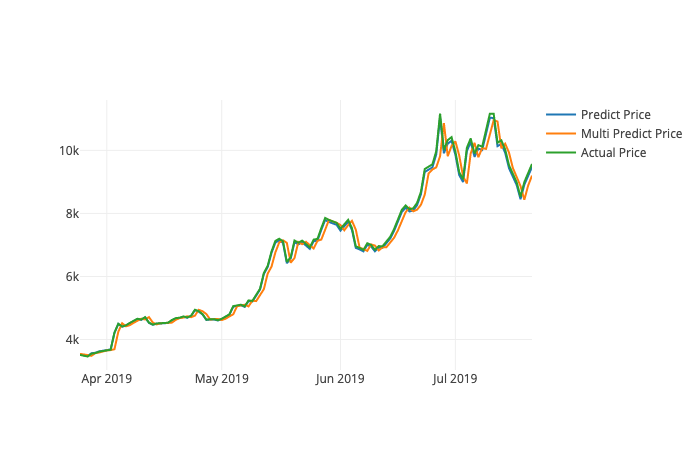
\includegraphics{8.png}
\end{figure}     
    
    The symmetric mean absolute percentage error (SMAPE) is:

    \begin{Verbatim}[commandchars=\\\{\}]
{\color{incolor}In [{\color{incolor}72}]:} \PY{k}{def} \PY{n+nf}{symmetric\PYZus{}mean\PYZus{}absolute\PYZus{}percentage\PYZus{}error}\PY{p}{(}\PY{n}{y\PYZus{}true}\PY{p}{,} \PY{n}{y\PYZus{}pred}\PY{p}{)}\PY{p}{:}
             \PY{k}{return} \PY{n}{np}\PY{o}{.}\PY{n}{mean}\PY{p}{(}\PY{n}{np}\PY{o}{.}\PY{n}{abs}\PY{p}{(}\PY{n}{y\PYZus{}pred} \PY{o}{\PYZhy{}} \PY{n}{y\PYZus{}true}\PY{p}{)} \PY{o}{/} \PY{p}{(}\PY{p}{(}\PY{n}{np}\PY{o}{.}\PY{n}{abs}\PY{p}{(}\PY{n}{y\PYZus{}true}\PY{p}{)} \PY{o}{+} \PY{n}{np}\PY{o}{.}\PY{n}{abs}\PY{p}{(}\PY{n}{y\PYZus{}pred}\PY{p}{)}\PY{p}{)}\PY{o}{/}\PY{l+m+mi}{2}\PY{p}{)}\PY{p}{)} \PY{o}{*} \PY{l+m+mi}{100}
         
         \PY{n}{SMAPE} \PY{o}{=} \PY{n}{symmetric\PYZus{}mean\PYZus{}absolute\PYZus{}percentage\PYZus{}error}\PY{p}{(}\PY{n}{inv\PYZus{}y}\PY{p}{,} \PY{n}{inv\PYZus{}yhat}\PY{p}{)}
         
         \PY{n+nb}{print}\PY{p}{(}\PY{l+s+s1}{\PYZsq{}}\PY{l+s+s1}{Test SMAPE (percentage): }\PY{l+s+si}{\PYZpc{}.3f}\PY{l+s+s1}{\PYZsq{}} \PY{o}{\PYZpc{}} \PY{n}{SMAPE}\PY{p}{)}
\end{Verbatim}

    \begin{Verbatim}[commandchars=\\\{\}]
Test SMAPE (percentage): 2.793

    \end{Verbatim}

    \hypertarget{arima}{%
\section{ARIMA}\label{arima}}

    A time series is a sequence where a metric is recorded over regular time
intervals. Forecasting a time series (like demand and sales) is often of
tremendous commercial value.

    A TS is said to be stationary if its statistical properties such as
mean, variance remain constant over time. But why is it important? Most
of the TS models work on the assumption that the TS is stationary.

    We can check stationarity using the following:

\begin{enumerate}
\def\labelenumi{\arabic{enumi}.}
\item
  \textbf{Plotting Rolling Statistics}: Plot the moving average or
  moving variance and see if it varies with time. By moving
  average/variance I mean that at any instant \emph{t}, we'll take the
  average/variance of the last year, i.e.~last 12 months (this is a
  visual technique)
\item
  \textbf{Dickey-Fuller Test}: This is one of the statistical tests for
  checking stationarity. Here the null hypothesis is that the time
  series is non-stationary. The test results comprise of a Test
  Statistic and some Critical Values for difference confidence levels.
  If the ``Test Statistic'' is less than the ``Critical Value'', we can
  reject the null hypothesis and say that the series is stationary.
  Statistical tests make strong assumptions about your data
\end{enumerate}

    \emph{Null Hypothesis (H0)}: If accepted, it suggests the time series
has a unit root, meaning it is non-stationary. It has some time
dependent structure.

    \emph{Alternate Hypothesis (H1)}: The null hypothesis is rejected, it
suggests the time series does not have a unit root, meaning it is
stationary. It does not have time-dependent structure. We interpret this
result using the p-value from the test.

    A p-value below a threshold (such as 5\% or 1\%) suggests we reject the
null hypothesis (stationary), otherwise a p-value above the threshold
suggests we accept the null hypothesis (non-stationary).

\begin{itemize}
\item
  \emph{p-value \textgreater{} 0.05}: Accept the null hypothesis
  \emph{(H0)}, the data has a unit root and is non-stationary.
\item
  \emph{p-value \textless= 0.05}: Reject the null hypothesis
  \emph{(H0)}, the data does not have a unit root and is stationary.
\end{itemize}

    \textbf{ARIMA} model is implemented to compare its predictability with
the LSTM and figure out which is the most suitable method for time
series data which has huge fluctuations.

    An ARIMA model is a class of statistical models for analyzing and
forecasting time series data. It explicitly caters to a suite of
standard structures in time series data, and as such provides a simple
yet powerful method for making skillful time series forecasts.

    ARIMA is an acronym that stands for AutoRegressive Integrated Moving
Average. It is a generalization of the simpler AutoRegressive Moving
Average and adds the notion of integration. This acronym is descriptive,
capturing the key aspects of the model itself. Briefly, they are:

\begin{itemize}
\tightlist
\item
  \textbf{AR}: Autoregression: A model that uses the dependent
  relationship between an observation and some number of lagged
  observations
\item
  \textbf{I}: Integrated: The use of differencing of raw observations
  (e.g.~subtracting an observation from an observation at the previous
  time step) in order to make the time series stationary
\item
  \textbf{MA}: Moving Average: A model that uses the dependency between
  an observation and a residual error from a moving average model
  applied to lagged observations
\end{itemize}

A standard notation is used of ARIMA (p, d, q) where the parameters are
substituted with integer values to quickly indicate the specific ARIMA
model being used.

    The parameters of the ARIMA model are defined as follows:

\begin{itemize}
\tightlist
\item
  \textbf{p}: The number of lag observations included in the model, also
  called the lag order
\item
  \textbf{d}: The number of times that the raw observations are
  differenced, also called the ``degree of differencing''
\item
  \textbf{q}: The size of the moving average window, also called the
  order of moving average
\end{itemize}

    A linear regression model is constructed including the specified number
and type of terms, and the data is prepared by a degree of differencing
in order to make it stationary, i.e.~to remove trend and seasonal
structures that negatively affect the regression model.

    An importance concern here is how to determine the value of `p' and `q'.
We use two plots to determine these numbers:

\begin{itemize}
\item
  \textbf{Autocorrelation Function (ACF)}: It is a measure of the
  correlation between the the TS with a lagged version of itself
\item
  \textbf{Partial Autocorrelation Function (PACF)}: This measures the
  correlation between the TS with a lagged version of itself but after
  eliminating the variations already explained by the intervening
  comparisons
\end{itemize}

    We import the required dependencies taking the \emph{Weighted Price}
data:

    \begin{Verbatim}[commandchars=\\\{\}]
{\color{incolor}In [{\color{incolor}73}]:} \PY{k+kn}{from} \PY{n+nn}{matplotlib}\PY{n+nn}{.}\PY{n+nn}{pylab} \PY{k}{import} \PY{n}{rcParams}
         \PY{k+kn}{from} \PY{n+nn}{statsmodels}\PY{n+nn}{.}\PY{n+nn}{tsa}\PY{n+nn}{.}\PY{n+nn}{arima\PYZus{}model} \PY{k}{import} \PY{n}{ARIMA}
         \PY{k+kn}{from} \PY{n+nn}{statsmodels}\PY{n+nn}{.}\PY{n+nn}{tsa}\PY{n+nn}{.}\PY{n+nn}{stattools} \PY{k}{import} \PY{n}{acf}\PY{p}{,} \PY{n}{pacf}
         \PY{k+kn}{from} \PY{n+nn}{statsmodels}\PY{n+nn}{.}\PY{n+nn}{tsa}\PY{n+nn}{.}\PY{n+nn}{stattools} \PY{k}{import} \PY{n}{adfuller}
\end{Verbatim}

    \begin{Verbatim}[commandchars=\\\{\}]
{\color{incolor}In [{\color{incolor}74}]:} \PY{n}{ts} \PY{o}{=} \PY{n}{data}\PY{p}{[}\PY{l+s+s1}{\PYZsq{}}\PY{l+s+s1}{Weighted Price}\PY{l+s+s1}{\PYZsq{}}\PY{p}{]}
\end{Verbatim}

    As we have said before,, the first important thing when forecasting time
series is to check if the data is stationary. This means that our data
is influenced by such factors as trend or seasonality.

    The seasonal component, given a ``period'', is the value of the
measurement under examination that is repeated the same for each period.

    The trend component, using the moving averages, is the one that
identifies the macroscopic trend of the series. In simple terms, the
trend shows whether compared to the seasonal trend, the value of the
measurement under examination is further rising or falling.

    The residual component is the noise which, as can be guessed,
corresponds to what remains of the value under examination by
subtracting the two previous components.

    We can see also the actual price movements (``observed'').

    \begin{Verbatim}[commandchars=\\\{\}]
{\color{incolor}In [{\color{incolor}75}]:} \PY{n}{s} \PY{o}{=} \PY{n}{sm}\PY{o}{.}\PY{n}{tsa}\PY{o}{.}\PY{n}{seasonal\PYZus{}decompose}\PY{p}{(}\PY{n}{btc\PYZus{}eur\PYZus{}price\PYZus{}kraken}\PY{p}{[}\PY{l+s+s1}{\PYZsq{}}\PY{l+s+s1}{Weighted Price}\PY{l+s+s1}{\PYZsq{}}\PY{p}{]}\PY{o}{.}\PY{n}{values}\PY{p}{,} \PY{n}{freq}\PY{o}{=}\PY{l+m+mi}{60}\PY{p}{)}
\end{Verbatim}

    \begin{Verbatim}[commandchars=\\\{\}]
{\color{incolor}In [{\color{incolor}76}]:} \PY{n}{trace1} \PY{o}{=} \PY{n}{go}\PY{o}{.}\PY{n}{Scatter}\PY{p}{(}\PY{n}{x} \PY{o}{=} \PY{n}{np}\PY{o}{.}\PY{n}{arange}\PY{p}{(}\PY{l+m+mi}{0}\PY{p}{,} \PY{n+nb}{len}\PY{p}{(}\PY{n}{s}\PY{o}{.}\PY{n}{trend}\PY{p}{)}\PY{p}{,} \PY{l+m+mi}{1}\PY{p}{)}\PY{p}{,}
                             \PY{n}{y} \PY{o}{=} \PY{n}{s}\PY{o}{.}\PY{n}{trend}\PY{p}{,}\PY{n}{mode} \PY{o}{=} \PY{l+s+s1}{\PYZsq{}}\PY{l+s+s1}{lines}\PY{l+s+s1}{\PYZsq{}}\PY{p}{,}\PY{n}{name} \PY{o}{=} \PY{l+s+s1}{\PYZsq{}}\PY{l+s+s1}{Trend}\PY{l+s+s1}{\PYZsq{}}\PY{p}{,}
             \PY{n}{line} \PY{o}{=} \PY{n+nb}{dict}\PY{p}{(}\PY{n}{color} \PY{o}{=} \PY{p}{(}\PY{l+s+s1}{\PYZsq{}}\PY{l+s+s1}{rgb(244, 146, 65)}\PY{l+s+s1}{\PYZsq{}}\PY{p}{)}\PY{p}{,} \PY{n}{width} \PY{o}{=} \PY{l+m+mi}{4}\PY{p}{)}\PY{p}{)}
         \PY{n}{trace2} \PY{o}{=} \PY{n}{go}\PY{o}{.}\PY{n}{Scatter}\PY{p}{(}\PY{n}{x} \PY{o}{=} \PY{n}{np}\PY{o}{.}\PY{n}{arange}\PY{p}{(}\PY{l+m+mi}{0}\PY{p}{,} \PY{n+nb}{len}\PY{p}{(}\PY{n}{s}\PY{o}{.}\PY{n}{seasonal}\PY{p}{)}\PY{p}{,} \PY{l+m+mi}{1}\PY{p}{)}\PY{p}{,}
                             \PY{n}{y} \PY{o}{=} \PY{n}{s}\PY{o}{.}\PY{n}{seasonal}\PY{p}{,}\PY{n}{mode} \PY{o}{=} \PY{l+s+s1}{\PYZsq{}}\PY{l+s+s1}{lines}\PY{l+s+s1}{\PYZsq{}}\PY{p}{,}\PY{n}{name} \PY{o}{=} \PY{l+s+s1}{\PYZsq{}}\PY{l+s+s1}{Seasonal}\PY{l+s+s1}{\PYZsq{}}\PY{p}{,}
             \PY{n}{line} \PY{o}{=} \PY{n+nb}{dict}\PY{p}{(}\PY{n}{color} \PY{o}{=} \PY{p}{(}\PY{l+s+s1}{\PYZsq{}}\PY{l+s+s1}{rgb(66, 244, 155)}\PY{l+s+s1}{\PYZsq{}}\PY{p}{)}\PY{p}{,} \PY{n}{width} \PY{o}{=} \PY{l+m+mi}{2}\PY{p}{)}\PY{p}{)}
         
         \PY{n}{trace3} \PY{o}{=} \PY{n}{go}\PY{o}{.}\PY{n}{Scatter}\PY{p}{(}\PY{n}{x} \PY{o}{=} \PY{n}{np}\PY{o}{.}\PY{n}{arange}\PY{p}{(}\PY{l+m+mi}{0}\PY{p}{,} \PY{n+nb}{len}\PY{p}{(}\PY{n}{s}\PY{o}{.}\PY{n}{resid}\PY{p}{)}\PY{p}{,} \PY{l+m+mi}{1}\PY{p}{)}\PY{p}{,}
                             \PY{n}{y} \PY{o}{=} \PY{n}{s}\PY{o}{.}\PY{n}{resid}\PY{p}{,}\PY{n}{mode} \PY{o}{=} \PY{l+s+s1}{\PYZsq{}}\PY{l+s+s1}{lines}\PY{l+s+s1}{\PYZsq{}}\PY{p}{,}\PY{n}{name} \PY{o}{=} \PY{l+s+s1}{\PYZsq{}}\PY{l+s+s1}{Residual}\PY{l+s+s1}{\PYZsq{}}\PY{p}{,}
             \PY{n}{line} \PY{o}{=} \PY{n+nb}{dict}\PY{p}{(}\PY{n}{color} \PY{o}{=} \PY{p}{(}\PY{l+s+s1}{\PYZsq{}}\PY{l+s+s1}{rgb(209, 244, 66)}\PY{l+s+s1}{\PYZsq{}}\PY{p}{)}\PY{p}{,} \PY{n}{width} \PY{o}{=} \PY{l+m+mi}{2}\PY{p}{)}\PY{p}{)}
         
         \PY{n}{trace4} \PY{o}{=} \PY{n}{go}\PY{o}{.}\PY{n}{Scatter}\PY{p}{(}\PY{n}{x} \PY{o}{=} \PY{n}{np}\PY{o}{.}\PY{n}{arange}\PY{p}{(}\PY{l+m+mi}{0}\PY{p}{,} \PY{n+nb}{len}\PY{p}{(}\PY{n}{s}\PY{o}{.}\PY{n}{observed}\PY{p}{)}\PY{p}{,} \PY{l+m+mi}{1}\PY{p}{)}\PY{p}{,}
                             \PY{n}{y} \PY{o}{=} \PY{n}{s}\PY{o}{.}\PY{n}{observed}\PY{p}{,}\PY{n}{mode} \PY{o}{=} \PY{l+s+s1}{\PYZsq{}}\PY{l+s+s1}{lines}\PY{l+s+s1}{\PYZsq{}}\PY{p}{,}\PY{n}{name} \PY{o}{=} \PY{l+s+s1}{\PYZsq{}}\PY{l+s+s1}{Observed}\PY{l+s+s1}{\PYZsq{}}\PY{p}{,}
             \PY{n}{line} \PY{o}{=} \PY{n+nb}{dict}\PY{p}{(}\PY{n}{color} \PY{o}{=} \PY{p}{(}\PY{l+s+s1}{\PYZsq{}}\PY{l+s+s1}{rgb(66, 134, 244)}\PY{l+s+s1}{\PYZsq{}}\PY{p}{)}\PY{p}{,} \PY{n}{width} \PY{o}{=} \PY{l+m+mi}{2}\PY{p}{)}\PY{p}{)}
         
         \PY{n}{data} \PY{o}{=} \PY{p}{[}\PY{n}{trace1}\PY{p}{,} \PY{n}{trace2}\PY{p}{,} \PY{n}{trace3}\PY{p}{,} \PY{n}{trace4}\PY{p}{]}
         \PY{n}{layout} \PY{o}{=} \PY{n+nb}{dict}\PY{p}{(}\PY{n}{title} \PY{o}{=} \PY{l+s+s1}{\PYZsq{}}\PY{l+s+s1}{Seasonal decomposition}\PY{l+s+s1}{\PYZsq{}}\PY{p}{,} \PY{n}{xaxis} \PY{o}{=} \PY{n+nb}{dict}\PY{p}{(}\PY{n}{title} \PY{o}{=} \PY{l+s+s1}{\PYZsq{}}\PY{l+s+s1}{Time}\PY{l+s+s1}{\PYZsq{}}\PY{p}{)}\PY{p}{,}
                       \PY{n}{yaxis} \PY{o}{=} \PY{n+nb}{dict}\PY{p}{(}\PY{n}{title} \PY{o}{=} \PY{l+s+s1}{\PYZsq{}}\PY{l+s+s1}{Price, USD}\PY{l+s+s1}{\PYZsq{}}\PY{p}{)}\PY{p}{)}
         \PY{n}{fig} \PY{o}{=} \PY{n+nb}{dict}\PY{p}{(}\PY{n}{data}\PY{o}{=}\PY{n}{data}\PY{p}{,} \PY{n}{layout}\PY{o}{=}\PY{n}{layout}\PY{p}{)}
         \PY{n}{plotly}\PY{o}{.}\PY{n}{offline}\PY{o}{.}\PY{n}{iplot}\PY{p}{(}\PY{n}{fig}\PY{p}{,} \PY{n}{filename}\PY{o}{=}\PY{l+s+s1}{\PYZsq{}}\PY{l+s+s1}{seasonal\PYZus{}decomposition}\PY{l+s+s1}{\PYZsq{}}\PY{p}{)}
\end{Verbatim}

\begin{figure}[H]
	\centering
		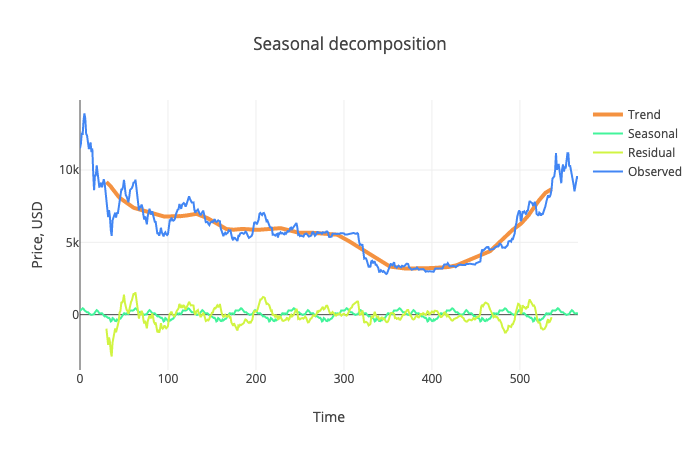
\includegraphics{9.png}
\end{figure}     
    
    Most business and economic time series are far from stationary when
expressed in their original units of measurement, and even after
diminution or seasonal adjustment they will typically still exhibit
trends, cycles, random-walking, and other non-stationary behavior. If
the series has a stable long-run trend and tends to revert to the trend
line following a disturbance, it may be possible to stationarize it by
de-trending (e.g.~including the time index as an independent variable in
a regression or ARIMA model). Such a series is said to be
trend-stationary.

    However, sometimes even de-trending is not sufficient to make the series
stationary, in which case it may be necessary to transform it into a
series of period-to-period and/or season-to-season differences. If the
mean, variance, and autocorrelations of the original series are not
constant in time, even after detrending, perhaps the statistics of the
changes in the series between periods or between seasons will be
constant. Such a series is said to be difference-stationary.

    The next thing we do is the examination of the autocorrelation. It is
the similarity between observations as a function of the time lag
between them. It is important for finding repeating patterns in the
data.

    \begin{Verbatim}[commandchars=\\\{\}]
{\color{incolor}In [{\color{incolor}77}]:} \PY{n}{plt}\PY{o}{.}\PY{n}{figure}\PY{p}{(}\PY{n}{figsize}\PY{o}{=}\PY{p}{(}\PY{l+m+mi}{13}\PY{p}{,}\PY{l+m+mi}{7}\PY{p}{)}\PY{p}{)}
         \PY{n}{ax} \PY{o}{=} \PY{n}{plt}\PY{o}{.}\PY{n}{subplot}\PY{p}{(}\PY{l+m+mi}{211}\PY{p}{)}
         \PY{n}{sm}\PY{o}{.}\PY{n}{graphics}\PY{o}{.}\PY{n}{tsa}\PY{o}{.}\PY{n}{plot\PYZus{}acf}\PY{p}{(}\PY{n}{btc\PYZus{}eur\PYZus{}price\PYZus{}kraken}\PY{p}{[}\PY{l+s+s1}{\PYZsq{}}\PY{l+s+s1}{Weighted Price}\PY{l+s+s1}{\PYZsq{}}\PY{p}{]}\PY{o}{.}\PY{n}{values}\PY{o}{.}\PY{n}{squeeze}\PY{p}{(}\PY{p}{)}\PY{p}{,}
                                  \PY{n}{lags}\PY{o}{=}\PY{l+m+mi}{48}\PY{p}{,} \PY{n}{ax}\PY{o}{=}\PY{n}{ax}\PY{p}{)}
         \PY{n}{ax} \PY{o}{=} \PY{n}{plt}\PY{o}{.}\PY{n}{subplot}\PY{p}{(}\PY{l+m+mi}{212}\PY{p}{)}
         \PY{n}{sm}\PY{o}{.}\PY{n}{graphics}\PY{o}{.}\PY{n}{tsa}\PY{o}{.}\PY{n}{plot\PYZus{}pacf}\PY{p}{(}\PY{n}{btc\PYZus{}eur\PYZus{}price\PYZus{}kraken}\PY{p}{[}\PY{l+s+s1}{\PYZsq{}}\PY{l+s+s1}{Weighted Price}\PY{l+s+s1}{\PYZsq{}}\PY{p}{]}\PY{o}{.}\PY{n}{values}\PY{o}{.}\PY{n}{squeeze}\PY{p}{(}\PY{p}{)}\PY{p}{,}
                                   \PY{n}{lags}\PY{o}{=}\PY{l+m+mi}{48}\PY{p}{,} \PY{n}{ax}\PY{o}{=}\PY{n}{ax}\PY{p}{)}
         \PY{n}{plt}\PY{o}{.}\PY{n}{tight\PYZus{}layout}\PY{p}{(}\PY{p}{)}
         \PY{n}{plt}\PY{o}{.}\PY{n}{show}\PY{p}{(}\PY{p}{)}
\end{Verbatim}

    \begin{center}
    \adjustimage{max size={0.9\linewidth}{0.9\paperheight}}{output_219_0.png}
    \end{center}
    { \hspace*{\fill} \\}
    
    In this plot, the two dotted lines on either sides of 0 are the
confidence intervals. These can be used to determine the \(p\) and \(q\)
values, parameters of the ARIMA model.

    We Determine rolling statistics and Perform Dickey-Fuller test.

    \begin{Verbatim}[commandchars=\\\{\}]
{\color{incolor}In [{\color{incolor}78}]:} \PY{k}{def} \PY{n+nf}{test\PYZus{}stationarity}\PY{p}{(}\PY{n}{timeseries}\PY{p}{)}\PY{p}{:}
             
             \PY{n}{rolmean} \PY{o}{=} \PY{n}{timeseries}\PY{o}{.}\PY{n}{rolling}\PY{p}{(}\PY{l+m+mi}{12}\PY{p}{)}\PY{o}{.}\PY{n}{mean}\PY{p}{(}\PY{p}{)}
             \PY{n}{rolstd} \PY{o}{=} \PY{n}{timeseries}\PY{o}{.}\PY{n}{rolling}\PY{p}{(}\PY{l+m+mi}{12}\PY{p}{)}\PY{o}{.}\PY{n}{std}\PY{p}{(}\PY{p}{)}
         
             \PY{n}{orig} \PY{o}{=} \PY{n}{plt}\PY{o}{.}\PY{n}{plot}\PY{p}{(}\PY{n}{timeseries}\PY{p}{,} \PY{n}{color}\PY{o}{=}\PY{l+s+s1}{\PYZsq{}}\PY{l+s+s1}{blue}\PY{l+s+s1}{\PYZsq{}}\PY{p}{,}\PY{n}{label}\PY{o}{=}\PY{l+s+s1}{\PYZsq{}}\PY{l+s+s1}{Original}\PY{l+s+s1}{\PYZsq{}}\PY{p}{)}
             \PY{n}{mean} \PY{o}{=} \PY{n}{plt}\PY{o}{.}\PY{n}{plot}\PY{p}{(}\PY{n}{rolmean}\PY{p}{,} \PY{n}{color}\PY{o}{=}\PY{l+s+s1}{\PYZsq{}}\PY{l+s+s1}{red}\PY{l+s+s1}{\PYZsq{}}\PY{p}{,} \PY{n}{label}\PY{o}{=}\PY{l+s+s1}{\PYZsq{}}\PY{l+s+s1}{Rolling Mean}\PY{l+s+s1}{\PYZsq{}}\PY{p}{)}
             \PY{n}{std} \PY{o}{=} \PY{n}{plt}\PY{o}{.}\PY{n}{plot}\PY{p}{(}\PY{n}{rolstd}\PY{p}{,} \PY{n}{color}\PY{o}{=}\PY{l+s+s1}{\PYZsq{}}\PY{l+s+s1}{black}\PY{l+s+s1}{\PYZsq{}}\PY{p}{,} \PY{n}{label} \PY{o}{=} \PY{l+s+s1}{\PYZsq{}}\PY{l+s+s1}{Rolling Std}\PY{l+s+s1}{\PYZsq{}}\PY{p}{)}
             \PY{n}{plt}\PY{o}{.}\PY{n}{legend}\PY{p}{(}\PY{n}{loc}\PY{o}{=}\PY{l+s+s1}{\PYZsq{}}\PY{l+s+s1}{best}\PY{l+s+s1}{\PYZsq{}}\PY{p}{)}
             \PY{n}{plt}\PY{o}{.}\PY{n}{title}\PY{p}{(}\PY{l+s+s1}{\PYZsq{}}\PY{l+s+s1}{Rolling Mean \PYZam{} Standard Deviation}\PY{l+s+s1}{\PYZsq{}}\PY{p}{)}
             \PY{n}{plt}\PY{o}{.}\PY{n}{show}\PY{p}{(}\PY{n}{block}\PY{o}{=}\PY{k+kc}{False}\PY{p}{)}
             
             \PY{n+nb}{print} \PY{p}{(}\PY{l+s+s1}{\PYZsq{}}\PY{l+s+s1}{Results of Dickey\PYZhy{}Fuller Test:}\PY{l+s+s1}{\PYZsq{}}\PY{p}{)}
             \PY{n}{dftest} \PY{o}{=} \PY{n}{adfuller}\PY{p}{(}\PY{n}{timeseries}\PY{p}{,} \PY{n}{autolag}\PY{o}{=}\PY{l+s+s1}{\PYZsq{}}\PY{l+s+s1}{AIC}\PY{l+s+s1}{\PYZsq{}}\PY{p}{)}
             \PY{n}{dfoutput} \PY{o}{=} \PY{n}{pd}\PY{o}{.}\PY{n}{Series}\PY{p}{(}\PY{n}{dftest}\PY{p}{[}\PY{l+m+mi}{0}\PY{p}{:}\PY{l+m+mi}{4}\PY{p}{]}\PY{p}{,}
             \PY{n}{index}\PY{o}{=}\PY{p}{[}\PY{l+s+s1}{\PYZsq{}}\PY{l+s+s1}{Test Statistic}\PY{l+s+s1}{\PYZsq{}}\PY{p}{,}\PY{l+s+s1}{\PYZsq{}}\PY{l+s+s1}{p\PYZhy{}value}\PY{l+s+s1}{\PYZsq{}}\PY{p}{,}\PY{l+s+s1}{\PYZsq{}}\PY{l+s+s1}{\PYZsh{}Lags Used}\PY{l+s+s1}{\PYZsq{}}\PY{p}{,}\PY{l+s+s1}{\PYZsq{}}\PY{l+s+s1}{Number of Observations Used}\PY{l+s+s1}{\PYZsq{}}\PY{p}{]}\PY{p}{)}
             \PY{k}{for} \PY{n}{key}\PY{p}{,}\PY{n}{value} \PY{o+ow}{in} \PY{n}{dftest}\PY{p}{[}\PY{l+m+mi}{4}\PY{p}{]}\PY{o}{.}\PY{n}{items}\PY{p}{(}\PY{p}{)}\PY{p}{:}
                 \PY{n}{dfoutput}\PY{p}{[}\PY{l+s+s1}{\PYZsq{}}\PY{l+s+s1}{Critical Value (}\PY{l+s+si}{\PYZpc{}s}\PY{l+s+s1}{)}\PY{l+s+s1}{\PYZsq{}}\PY{o}{\PYZpc{}}\PY{k}{key}] = value
             \PY{n+nb}{print} \PY{p}{(}\PY{n}{dfoutput}\PY{p}{)}
\end{Verbatim}

    \begin{Verbatim}[commandchars=\\\{\}]
{\color{incolor}In [{\color{incolor}79}]:} \PY{k+kn}{from} \PY{n+nn}{pandas}\PY{n+nn}{.}\PY{n+nn}{plotting} \PY{k}{import} \PY{n}{register\PYZus{}matplotlib\PYZus{}converters}
         \PY{n}{register\PYZus{}matplotlib\PYZus{}converters}\PY{p}{(}\PY{p}{)}
         \PY{n}{rcParams}\PY{p}{[}\PY{l+s+s1}{\PYZsq{}}\PY{l+s+s1}{figure.figsize}\PY{l+s+s1}{\PYZsq{}}\PY{p}{]} \PY{o}{=} \PY{l+m+mi}{30}\PY{p}{,} \PY{l+m+mi}{15}
         \PY{n}{test\PYZus{}stationarity}\PY{p}{(}\PY{n}{ts}\PY{p}{)}
\end{Verbatim}

    \begin{center}
    \adjustimage{max size={0.9\linewidth}{0.9\paperheight}}{output_223_0.png}
    \end{center}
    { \hspace*{\fill} \\}
    
    \begin{Verbatim}[commandchars=\\\{\}]
Results of Dickey-Fuller Test:
Test Statistic                  -1.827799
p-value                          0.366750
\#Lags Used                      17.000000
Number of Observations Used    549.000000
Critical Value (1\%)             -3.442317
Critical Value (5\%)             -2.866819
Critical Value (10\%)            -2.569582
dtype: float64

    \end{Verbatim}

    The series isn't stationary. There are two major reasons behind
non-stationarity of a TS:

\begin{enumerate}
\def\labelenumi{\arabic{enumi}.}
\tightlist
\item
  Trend: varying mean over time
\item
  Seasonality: variations at specific time-frames
\end{enumerate}

    There are two ways of removing trend and seasonality:

\begin{itemize}
\tightlist
\item
  Differencing: taking the differece with a particular time lag
\item
  Decomposition: modeling both trend and seasonality and removing them
  from the model.
\end{itemize}

    One of the most common methods of dealing with both trend and
seasonality is differencing. In this technique, we take the difference
of the observation at a particular instant with that at the previous
instant. This mostly works well in improving stationarity.

    Log transformation is used to unskew highly skewed data, thus helping in
forecasting process.

    \begin{Verbatim}[commandchars=\\\{\}]
{\color{incolor}In [{\color{incolor}80}]:} \PY{n}{ts\PYZus{}log} \PY{o}{=} \PY{n}{np}\PY{o}{.}\PY{n}{log}\PY{p}{(}\PY{n}{ts}\PY{p}{)}
         \PY{n}{plt}\PY{o}{.}\PY{n}{plot}\PY{p}{(}\PY{n}{ts\PYZus{}log}\PY{p}{)}
         \PY{n}{plt}\PY{o}{.}\PY{n}{show}\PY{p}{(}\PY{p}{)}
\end{Verbatim}

    \begin{center}
    \adjustimage{max size={0.9\linewidth}{0.9\paperheight}}{output_228_0.png}
    \end{center}
    { \hspace*{\fill} \\}
    
    First order differencing can be done in Pandas as:

    \begin{Verbatim}[commandchars=\\\{\}]
{\color{incolor}In [{\color{incolor}81}]:} \PY{n}{ts\PYZus{}log\PYZus{}diff} \PY{o}{=} \PY{n}{ts\PYZus{}log} \PY{o}{\PYZhy{}} \PY{n}{ts\PYZus{}log}\PY{o}{.}\PY{n}{shift}\PY{p}{(}\PY{p}{)}
         \PY{n}{plt}\PY{o}{.}\PY{n}{plot}\PY{p}{(}\PY{n}{ts\PYZus{}log\PYZus{}diff}\PY{p}{)}
         \PY{n}{plt}\PY{o}{.}\PY{n}{show}\PY{p}{(}\PY{p}{)}
\end{Verbatim}

    \begin{center}
    \adjustimage{max size={0.9\linewidth}{0.9\paperheight}}{output_230_0.png}
    \end{center}
    { \hspace*{\fill} \\}
    
    This appears to have reduced trend considerably. Let's verify using our
plots:

    \begin{Verbatim}[commandchars=\\\{\}]
{\color{incolor}In [{\color{incolor}82}]:} \PY{n}{ts\PYZus{}log\PYZus{}diff}\PY{o}{.}\PY{n}{dropna}\PY{p}{(}\PY{n}{inplace}\PY{o}{=}\PY{k+kc}{True}\PY{p}{)}
         \PY{n}{test\PYZus{}stationarity}\PY{p}{(}\PY{n}{ts\PYZus{}log\PYZus{}diff}\PY{p}{)}
\end{Verbatim}

    \begin{center}
    \adjustimage{max size={0.9\linewidth}{0.9\paperheight}}{output_232_0.png}
    \end{center}
    { \hspace*{\fill} \\}
    
    \begin{Verbatim}[commandchars=\\\{\}]
Results of Dickey-Fuller Test:
Test Statistic                -1.277924e+01
p-value                        7.477214e-24
\#Lags Used                     2.000000e+00
Number of Observations Used    5.630000e+02
Critical Value (1\%)           -3.442019e+00
Critical Value (5\%)           -2.866687e+00
Critical Value (10\%)          -2.569511e+00
dtype: float64

    \end{Verbatim}

    Now the current time series is stationary.

    The ACF and PACF plots for the TS after differencing can be plotted as:

    \begin{Verbatim}[commandchars=\\\{\}]
{\color{incolor}In [{\color{incolor}83}]:} \PY{n}{lag\PYZus{}acf} \PY{o}{=} \PY{n}{acf}\PY{p}{(}\PY{n}{ts\PYZus{}log\PYZus{}diff}\PY{p}{,} \PY{n}{nlags}\PY{o}{=}\PY{l+m+mi}{20}\PY{p}{)}
         \PY{n}{lag\PYZus{}pacf} \PY{o}{=} \PY{n}{pacf}\PY{p}{(}\PY{n}{ts\PYZus{}log\PYZus{}diff}\PY{p}{,} \PY{n}{nlags}\PY{o}{=}\PY{l+m+mi}{20}\PY{p}{,} \PY{n}{method}\PY{o}{=}\PY{l+s+s1}{\PYZsq{}}\PY{l+s+s1}{ols}\PY{l+s+s1}{\PYZsq{}}\PY{p}{)}
\end{Verbatim}

    \begin{Verbatim}[commandchars=\\\{\}]
{\color{incolor}In [{\color{incolor}84}]:} \PY{n}{plt}\PY{o}{.}\PY{n}{plot}\PY{p}{(}\PY{n}{lag\PYZus{}acf}\PY{p}{)}
         \PY{n}{plt}\PY{o}{.}\PY{n}{axhline}\PY{p}{(}\PY{n}{y}\PY{o}{=}\PY{l+m+mi}{0}\PY{p}{,}\PY{n}{linestyle}\PY{o}{=}\PY{l+s+s1}{\PYZsq{}}\PY{l+s+s1}{\PYZhy{}\PYZhy{}}\PY{l+s+s1}{\PYZsq{}}\PY{p}{,}\PY{n}{color}\PY{o}{=}\PY{l+s+s1}{\PYZsq{}}\PY{l+s+s1}{gray}\PY{l+s+s1}{\PYZsq{}}\PY{p}{)}
         \PY{n}{plt}\PY{o}{.}\PY{n}{axhline}\PY{p}{(}\PY{n}{y}\PY{o}{=}\PY{o}{\PYZhy{}}\PY{l+m+mf}{1.96}\PY{o}{/}\PY{n}{np}\PY{o}{.}\PY{n}{sqrt}\PY{p}{(}\PY{n+nb}{len}\PY{p}{(}\PY{n}{ts\PYZus{}log\PYZus{}diff}\PY{p}{)}\PY{p}{)}\PY{p}{,}\PY{n}{linestyle}\PY{o}{=}\PY{l+s+s1}{\PYZsq{}}\PY{l+s+s1}{\PYZhy{}\PYZhy{}}\PY{l+s+s1}{\PYZsq{}}\PY{p}{,}\PY{n}{color}\PY{o}{=}\PY{l+s+s1}{\PYZsq{}}\PY{l+s+s1}{gray}\PY{l+s+s1}{\PYZsq{}}\PY{p}{)}
         \PY{n}{plt}\PY{o}{.}\PY{n}{axhline}\PY{p}{(}\PY{n}{y}\PY{o}{=}\PY{l+m+mf}{1.96}\PY{o}{/}\PY{n}{np}\PY{o}{.}\PY{n}{sqrt}\PY{p}{(}\PY{n+nb}{len}\PY{p}{(}\PY{n}{ts\PYZus{}log\PYZus{}diff}\PY{p}{)}\PY{p}{)}\PY{p}{,}\PY{n}{linestyle}\PY{o}{=}\PY{l+s+s1}{\PYZsq{}}\PY{l+s+s1}{\PYZhy{}\PYZhy{}}\PY{l+s+s1}{\PYZsq{}}\PY{p}{,}\PY{n}{color}\PY{o}{=}\PY{l+s+s1}{\PYZsq{}}\PY{l+s+s1}{gray}\PY{l+s+s1}{\PYZsq{}}\PY{p}{)}
         \PY{n}{plt}\PY{o}{.}\PY{n}{title}\PY{p}{(}\PY{l+s+s1}{\PYZsq{}}\PY{l+s+s1}{Autocorrelation Function}\PY{l+s+s1}{\PYZsq{}}\PY{p}{)}
         \PY{n}{plt}\PY{o}{.}\PY{n}{show}\PY{p}{(}\PY{p}{)}
\end{Verbatim}

    \begin{center}
    \adjustimage{max size={0.9\linewidth}{0.9\paperheight}}{output_236_0.png}
    \end{center}
    { \hspace*{\fill} \\}
    
    \begin{Verbatim}[commandchars=\\\{\}]
{\color{incolor}In [{\color{incolor}85}]:} \PY{n}{plt}\PY{o}{.}\PY{n}{plot}\PY{p}{(}\PY{n}{lag\PYZus{}pacf}\PY{p}{)}
         \PY{n}{plt}\PY{o}{.}\PY{n}{axhline}\PY{p}{(}\PY{n}{y}\PY{o}{=}\PY{l+m+mi}{0}\PY{p}{,}\PY{n}{linestyle}\PY{o}{=}\PY{l+s+s1}{\PYZsq{}}\PY{l+s+s1}{\PYZhy{}\PYZhy{}}\PY{l+s+s1}{\PYZsq{}}\PY{p}{,}\PY{n}{color}\PY{o}{=}\PY{l+s+s1}{\PYZsq{}}\PY{l+s+s1}{gray}\PY{l+s+s1}{\PYZsq{}}\PY{p}{)}
         \PY{n}{plt}\PY{o}{.}\PY{n}{axhline}\PY{p}{(}\PY{n}{y}\PY{o}{=}\PY{o}{\PYZhy{}}\PY{l+m+mf}{1.96}\PY{o}{/}\PY{n}{np}\PY{o}{.}\PY{n}{sqrt}\PY{p}{(}\PY{n+nb}{len}\PY{p}{(}\PY{n}{ts\PYZus{}log\PYZus{}diff}\PY{p}{)}\PY{p}{)}\PY{p}{,}\PY{n}{linestyle}\PY{o}{=}\PY{l+s+s1}{\PYZsq{}}\PY{l+s+s1}{\PYZhy{}\PYZhy{}}\PY{l+s+s1}{\PYZsq{}}\PY{p}{,}\PY{n}{color}\PY{o}{=}\PY{l+s+s1}{\PYZsq{}}\PY{l+s+s1}{gray}\PY{l+s+s1}{\PYZsq{}}\PY{p}{)}
         \PY{n}{plt}\PY{o}{.}\PY{n}{axhline}\PY{p}{(}\PY{n}{y}\PY{o}{=}\PY{l+m+mf}{1.96}\PY{o}{/}\PY{n}{np}\PY{o}{.}\PY{n}{sqrt}\PY{p}{(}\PY{n+nb}{len}\PY{p}{(}\PY{n}{ts\PYZus{}log\PYZus{}diff}\PY{p}{)}\PY{p}{)}\PY{p}{,}\PY{n}{linestyle}\PY{o}{=}\PY{l+s+s1}{\PYZsq{}}\PY{l+s+s1}{\PYZhy{}\PYZhy{}}\PY{l+s+s1}{\PYZsq{}}\PY{p}{,}\PY{n}{color}\PY{o}{=}\PY{l+s+s1}{\PYZsq{}}\PY{l+s+s1}{gray}\PY{l+s+s1}{\PYZsq{}}\PY{p}{)}
         \PY{n}{plt}\PY{o}{.}\PY{n}{title}\PY{p}{(}\PY{l+s+s1}{\PYZsq{}}\PY{l+s+s1}{Partial Autocorrelation Function}\PY{l+s+s1}{\PYZsq{}}\PY{p}{)}
         \PY{n}{plt}\PY{o}{.}\PY{n}{tight\PYZus{}layout}\PY{p}{(}\PY{p}{)}
         \PY{n}{plt}\PY{o}{.}\PY{n}{show}\PY{p}{(}\PY{p}{)}
\end{Verbatim}

    \begin{center}
    \adjustimage{max size={0.9\linewidth}{0.9\paperheight}}{output_237_0.png}
    \end{center}
    { \hspace*{\fill} \\}
    
    In this plot, the two dotted lines on either sides of 0 are the
confidence intervals. These can be used to determine the `p' and `q'
values as:

\emph{p}: The lag value where the PACF chart crosses the upper
confidence interval for the first time. If you notice closely, in this
case p=2

\emph{q}: The lag value where the ACF chart crosses the upper confidence
interval for the first time. If you notice closely, in this case q=2

    Now let's predict the last value in the data (Train and Test) with the
values p, d and q, the last value in the data and for the next 5 days.

    \hypertarget{predicting-the-last-value-in-the-data-train-and-test}{%
\subsection{Predicting the last value in the data (Train and
Test)}\label{predicting-the-last-value-in-the-data-train-and-test}}

    \begin{Verbatim}[commandchars=\\\{\}]
{\color{incolor}In [{\color{incolor}86}]:} \PY{n}{X} \PY{o}{=} \PY{n}{ts}\PY{o}{.}\PY{n}{values}
         
         \PY{n}{train\PYZus{}size} \PY{o}{=} \PY{n+nb}{int}\PY{p}{(}\PY{n+nb}{len}\PY{p}{(}\PY{n}{X}\PY{p}{)} \PY{o}{*} \PY{l+m+mf}{0.7}\PY{p}{)}
         \PY{n}{train}\PY{p}{,} \PY{n}{test} \PY{o}{=} \PY{n}{X}\PY{p}{[}\PY{l+m+mi}{0}\PY{p}{:}\PY{n}{train\PYZus{}size}\PY{p}{]}\PY{p}{,} \PY{n}{X}\PY{p}{[}\PY{n}{train\PYZus{}size}\PY{p}{:}\PY{p}{]}
         
         \PY{n}{model} \PY{o}{=} \PY{n}{ARIMA}\PY{p}{(}\PY{n}{train}\PY{p}{,} \PY{n}{order}\PY{o}{=}\PY{p}{(}\PY{l+m+mi}{2}\PY{p}{,}\PY{l+m+mi}{1}\PY{p}{,}\PY{l+m+mi}{2}\PY{p}{)}\PY{p}{)}
         \PY{n}{model\PYZus{}fit} \PY{o}{=} \PY{n}{model}\PY{o}{.}\PY{n}{fit}\PY{p}{(}\PY{n}{disp}\PY{o}{=}\PY{k+kc}{False}\PY{p}{)}
         \PY{n}{forecast}\PY{p}{,} \PY{n}{stderr}\PY{p}{,} \PY{n}{conf} \PY{o}{=} \PY{n}{model\PYZus{}fit}\PY{o}{.}\PY{n}{forecast}\PY{p}{(}\PY{p}{)}
         \PY{n+nb}{print}\PY{p}{(}\PY{l+s+s1}{\PYZsq{}}\PY{l+s+s1}{Expected: }\PY{l+s+si}{\PYZpc{}.3f}\PY{l+s+s1}{\PYZsq{}} \PY{o}{\PYZpc{}} \PY{n}{test}\PY{p}{[}\PY{l+m+mi}{0}\PY{p}{]}\PY{p}{)}
         \PY{n+nb}{print}\PY{p}{(}\PY{l+s+s1}{\PYZsq{}}\PY{l+s+s1}{Forecast: }\PY{l+s+si}{\PYZpc{}.3f}\PY{l+s+s1}{\PYZsq{}} \PY{o}{\PYZpc{}} \PY{n}{forecast}\PY{p}{)}
         \PY{n+nb}{print}\PY{p}{(}\PY{l+s+s1}{\PYZsq{}}\PY{l+s+s1}{Standard Error: }\PY{l+s+si}{\PYZpc{}.3f}\PY{l+s+s1}{\PYZsq{}} \PY{o}{\PYZpc{}} \PY{n}{stderr}\PY{p}{)}
         \PY{n+nb}{print}\PY{p}{(}\PY{l+s+s1}{\PYZsq{}}\PY{l+s+s1}{95}\PY{l+s+si}{\PYZpc{}\PYZpc{}}\PY{l+s+s1}{ Confidence Interval: }\PY{l+s+si}{\PYZpc{}.3f}\PY{l+s+s1}{ to }\PY{l+s+si}{\PYZpc{}.3f}\PY{l+s+s1}{\PYZsq{}} \PY{o}{\PYZpc{}} \PY{p}{(}\PY{n}{conf}\PY{p}{[}\PY{l+m+mi}{0}\PY{p}{]}\PY{p}{[}\PY{l+m+mi}{0}\PY{p}{]}\PY{p}{,} \PY{n}{conf}\PY{p}{[}\PY{l+m+mi}{0}\PY{p}{]}\PY{p}{[}\PY{l+m+mi}{1}\PY{p}{]}\PY{p}{)}\PY{p}{)}
\end{Verbatim}

    \begin{Verbatim}[commandchars=\\\{\}]
Expected: 2984.905
Forecast: 2969.036
Standard Error: 260.024
95\% Confidence Interval: 2459.398 to 3478.674

    \end{Verbatim}

    Confidence level determines the band in which we can safely say the
predicted and actual values can lie.

    We also calculate the MAE, MSE and RMSE.

    \begin{Verbatim}[commandchars=\\\{\}]
{\color{incolor}In [{\color{incolor}87}]:} \PY{n}{mae} \PY{o}{=} \PY{n}{mean\PYZus{}absolute\PYZus{}error}\PY{p}{(}\PY{n}{test}\PY{o}{.}\PY{n}{shape}\PY{p}{,} \PY{n}{forecast}\PY{o}{.}\PY{n}{shape}\PY{p}{)}
         \PY{n+nb}{print}\PY{p}{(}\PY{l+s+s1}{\PYZsq{}}\PY{l+s+s1}{MAE: }\PY{l+s+si}{\PYZpc{}.3f}\PY{l+s+s1}{\PYZsq{}} \PY{o}{\PYZpc{}} \PY{n}{mae}\PY{p}{)}
         \PY{n}{mse} \PY{o}{=} \PY{n}{mean\PYZus{}squared\PYZus{}error}\PY{p}{(}\PY{n}{test}\PY{o}{.}\PY{n}{shape}\PY{p}{,} \PY{n}{forecast}\PY{o}{.}\PY{n}{shape}\PY{p}{)}
         \PY{n+nb}{print}\PY{p}{(}\PY{l+s+s1}{\PYZsq{}}\PY{l+s+s1}{MSE: }\PY{l+s+si}{\PYZpc{}.3f}\PY{l+s+s1}{\PYZsq{}} \PY{o}{\PYZpc{}} \PY{n}{mse}\PY{p}{)}
         \PY{n}{rmse} \PY{o}{=} \PY{n}{sqrt}\PY{p}{(}\PY{n}{mse}\PY{p}{)}
         \PY{n+nb}{print}\PY{p}{(}\PY{l+s+s1}{\PYZsq{}}\PY{l+s+s1}{RMSE: }\PY{l+s+si}{\PYZpc{}.3f}\PY{l+s+s1}{\PYZsq{}} \PY{o}{\PYZpc{}} \PY{n}{rmse}\PY{p}{)}
\end{Verbatim}

    \begin{Verbatim}[commandchars=\\\{\}]
MAE: 170.000
MSE: 28900.000
RMSE: 170.000

    \end{Verbatim}

    \begin{Verbatim}[commandchars=\\\{\}]
{\color{incolor}In [{\color{incolor}88}]:} \PY{n}{X} \PY{o}{=} \PY{n}{ts}\PY{o}{.}\PY{n}{values}
         
         \PY{n}{train\PYZus{}size} \PY{o}{=} \PY{n+nb}{int}\PY{p}{(}\PY{n+nb}{len}\PY{p}{(}\PY{n}{X}\PY{p}{)} \PY{o}{*} \PY{l+m+mf}{0.7}\PY{p}{)}
         \PY{n}{train}\PY{p}{,} \PY{n}{test} \PY{o}{=} \PY{n}{X}\PY{p}{[}\PY{l+m+mi}{0}\PY{p}{:}\PY{n}{train\PYZus{}size}\PY{p}{]}\PY{p}{,} \PY{n}{X}\PY{p}{[}\PY{n}{train\PYZus{}size}\PY{p}{:}\PY{p}{]}
         
         \PY{n}{model} \PY{o}{=} \PY{n}{ARIMA}\PY{p}{(}\PY{n}{train}\PY{p}{,} \PY{n}{order}\PY{o}{=}\PY{p}{(}\PY{l+m+mi}{2}\PY{p}{,}\PY{l+m+mi}{1}\PY{p}{,}\PY{l+m+mi}{2}\PY{p}{)}\PY{p}{)}
         \PY{n}{model\PYZus{}fit} \PY{o}{=} \PY{n}{model}\PY{o}{.}\PY{n}{fit}\PY{p}{(}\PY{n}{disp}\PY{o}{=}\PY{k+kc}{False}\PY{p}{)}
         \PY{n}{intervals} \PY{o}{=} \PY{p}{[}\PY{l+m+mf}{0.2}\PY{p}{,} \PY{l+m+mf}{0.1}\PY{p}{,} \PY{l+m+mf}{0.05}\PY{p}{,} \PY{l+m+mf}{0.01}\PY{p}{]}
         \PY{k}{for} \PY{n}{a} \PY{o+ow}{in} \PY{n}{intervals}\PY{p}{:}
             \PY{n}{forecast}\PY{p}{,} \PY{n}{stderr}\PY{p}{,} \PY{n}{conf} \PY{o}{=} \PY{n}{model\PYZus{}fit}\PY{o}{.}\PY{n}{forecast}\PY{p}{(}\PY{n}{alpha}\PY{o}{=}\PY{n}{a}\PY{p}{)}
             \PY{n+nb}{print}\PY{p}{(}\PY{l+s+s1}{\PYZsq{}}\PY{l+s+si}{\PYZpc{}.1f}\PY{l+s+si}{\PYZpc{}\PYZpc{}}\PY{l+s+s1}{ Confidence Interval: }\PY{l+s+si}{\PYZpc{}.3f}\PY{l+s+s1}{ between }\PY{l+s+si}{\PYZpc{}.3f}\PY{l+s+s1}{ and }\PY{l+s+si}{\PYZpc{}.3f}\PY{l+s+s1}{\PYZsq{}} \PY{o}{\PYZpc{}} \PY{p}{(}\PY{p}{(}\PY{l+m+mi}{1}\PY{o}{\PYZhy{}}\PY{n}{a}\PY{p}{)}\PY{o}{*}\PY{l+m+mi}{100}\PY{p}{,} 
             \PY{n}{forecast}\PY{p}{,} \PY{n}{conf}\PY{p}{[}\PY{l+m+mi}{0}\PY{p}{]}\PY{p}{[}\PY{l+m+mi}{0}\PY{p}{]}\PY{p}{,} \PY{n}{conf}\PY{p}{[}\PY{l+m+mi}{0}\PY{p}{]}\PY{p}{[}\PY{l+m+mi}{1}\PY{p}{]}\PY{p}{)}\PY{p}{)}
\end{Verbatim}

    \begin{Verbatim}[commandchars=\\\{\}]
80.0\% Confidence Interval: 2969.036 between 2635.802 and 3302.271
90.0\% Confidence Interval: 2969.036 between 2541.335 and 3396.738
95.0\% Confidence Interval: 2969.036 between 2459.398 and 3478.674
99.0\% Confidence Interval: 2969.036 between 2299.259 and 3638.814

    \end{Verbatim}

    Now we predict the last value and predictions for the next 5 days.

    \hypertarget{predicting-the-last-value-in-the-data}{%
\subsection{Predicting the last value in the
data}\label{predicting-the-last-value-in-the-data}}

    \begin{Verbatim}[commandchars=\\\{\}]
{\color{incolor}In [{\color{incolor}89}]:} \PY{n}{X} \PY{o}{=} \PY{n}{ts}\PY{o}{.}\PY{n}{values}
         \PY{n}{size} \PY{o}{=} \PY{n+nb}{len}\PY{p}{(}\PY{n}{X}\PY{p}{)} \PY{o}{\PYZhy{}} \PY{l+m+mi}{1}
         \PY{n}{train}\PY{p}{,} \PY{n}{test} \PY{o}{=} \PY{n}{X}\PY{p}{[}\PY{l+m+mi}{0}\PY{p}{:}\PY{n}{size}\PY{p}{]}\PY{p}{,} \PY{n}{X}\PY{p}{[}\PY{n}{size}\PY{p}{:}\PY{p}{]}
         \PY{n}{model} \PY{o}{=} \PY{n}{ARIMA}\PY{p}{(}\PY{n}{train}\PY{p}{,} \PY{n}{order}\PY{o}{=}\PY{p}{(}\PY{l+m+mi}{2}\PY{p}{,}\PY{l+m+mi}{1}\PY{p}{,}\PY{l+m+mi}{2}\PY{p}{)}\PY{p}{)}
         \PY{n}{model\PYZus{}fit} \PY{o}{=} \PY{n}{model}\PY{o}{.}\PY{n}{fit}\PY{p}{(}\PY{n}{disp}\PY{o}{=}\PY{k+kc}{False}\PY{p}{)}
         \PY{n}{forecast}\PY{p}{,} \PY{n}{stderr}\PY{p}{,} \PY{n}{conf} \PY{o}{=} \PY{n}{model\PYZus{}fit}\PY{o}{.}\PY{n}{forecast}\PY{p}{(}\PY{p}{)}
         \PY{n+nb}{print}\PY{p}{(}\PY{l+s+s1}{\PYZsq{}}\PY{l+s+s1}{Expected: }\PY{l+s+si}{\PYZpc{}.3f}\PY{l+s+s1}{\PYZsq{}} \PY{o}{\PYZpc{}} \PY{n}{test}\PY{p}{)}
         \PY{n+nb}{print}\PY{p}{(}\PY{l+s+s1}{\PYZsq{}}\PY{l+s+s1}{Forecast: }\PY{l+s+si}{\PYZpc{}.3f}\PY{l+s+s1}{\PYZsq{}} \PY{o}{\PYZpc{}} \PY{n}{forecast}\PY{p}{)}
         \PY{n+nb}{print}\PY{p}{(}\PY{l+s+s1}{\PYZsq{}}\PY{l+s+s1}{Standard Error: }\PY{l+s+si}{\PYZpc{}.3f}\PY{l+s+s1}{\PYZsq{}} \PY{o}{\PYZpc{}} \PY{n}{stderr}\PY{p}{)}
         \PY{n+nb}{print}\PY{p}{(}\PY{l+s+s1}{\PYZsq{}}\PY{l+s+s1}{95}\PY{l+s+si}{\PYZpc{}\PYZpc{}}\PY{l+s+s1}{ Confidence Interval: }\PY{l+s+si}{\PYZpc{}.3f}\PY{l+s+s1}{ to }\PY{l+s+si}{\PYZpc{}.3f}\PY{l+s+s1}{\PYZsq{}} \PY{o}{\PYZpc{}} \PY{p}{(}\PY{n}{conf}\PY{p}{[}\PY{l+m+mi}{0}\PY{p}{]}\PY{p}{[}\PY{l+m+mi}{0}\PY{p}{]}\PY{p}{,} \PY{n}{conf}\PY{p}{[}\PY{l+m+mi}{0}\PY{p}{]}\PY{p}{[}\PY{l+m+mi}{1}\PY{p}{]}\PY{p}{)}\PY{p}{)}
\end{Verbatim}

    \begin{Verbatim}[commandchars=\\\{\}]
Expected: 9407.246
Forecast: 9634.719
Standard Error: 261.926
95\% Confidence Interval: 9121.353 to 10148.085

    \end{Verbatim}

    \begin{Verbatim}[commandchars=\\\{\}]
{\color{incolor}In [{\color{incolor}90}]:} \PY{n}{mae} \PY{o}{=} \PY{n}{mean\PYZus{}absolute\PYZus{}error}\PY{p}{(}\PY{n}{test}\PY{p}{,} \PY{n}{forecast}\PY{p}{)}
         \PY{n+nb}{print}\PY{p}{(}\PY{l+s+s1}{\PYZsq{}}\PY{l+s+s1}{MAE: }\PY{l+s+si}{\PYZpc{}.3f}\PY{l+s+s1}{\PYZsq{}} \PY{o}{\PYZpc{}} \PY{n}{mae}\PY{p}{)}
         \PY{n}{mse} \PY{o}{=} \PY{n}{mean\PYZus{}squared\PYZus{}error}\PY{p}{(}\PY{n}{test}\PY{p}{,} \PY{n}{forecast}\PY{p}{)}
         \PY{n+nb}{print}\PY{p}{(}\PY{l+s+s1}{\PYZsq{}}\PY{l+s+s1}{MSE: }\PY{l+s+si}{\PYZpc{}.3f}\PY{l+s+s1}{\PYZsq{}} \PY{o}{\PYZpc{}} \PY{n}{mse}\PY{p}{)}
         \PY{n}{rmse} \PY{o}{=} \PY{n}{sqrt}\PY{p}{(}\PY{n}{mse}\PY{p}{)}
         \PY{n+nb}{print}\PY{p}{(}\PY{l+s+s1}{\PYZsq{}}\PY{l+s+s1}{RMSE: }\PY{l+s+si}{\PYZpc{}.3f}\PY{l+s+s1}{\PYZsq{}} \PY{o}{\PYZpc{}} \PY{n}{rmse}\PY{p}{)}
\end{Verbatim}

    \begin{Verbatim}[commandchars=\\\{\}]
MAE: 227.473
MSE: 51744.148
RMSE: 227.473

    \end{Verbatim}

    \begin{Verbatim}[commandchars=\\\{\}]
{\color{incolor}In [{\color{incolor}91}]:} \PY{n}{X} \PY{o}{=} \PY{n}{ts}\PY{o}{.}\PY{n}{values}
         \PY{n}{size} \PY{o}{=} \PY{n+nb}{len}\PY{p}{(}\PY{n}{X}\PY{p}{)} \PY{o}{\PYZhy{}} \PY{l+m+mi}{1}
         \PY{n}{train}\PY{p}{,} \PY{n}{test} \PY{o}{=} \PY{n}{X}\PY{p}{[}\PY{l+m+mi}{0}\PY{p}{:}\PY{n}{size}\PY{p}{]}\PY{p}{,} \PY{n}{X}\PY{p}{[}\PY{n}{size}\PY{p}{:}\PY{p}{]}
         \PY{n}{model} \PY{o}{=} \PY{n}{ARIMA}\PY{p}{(}\PY{n}{train}\PY{p}{,} \PY{n}{order}\PY{o}{=}\PY{p}{(}\PY{l+m+mi}{2}\PY{p}{,}\PY{l+m+mi}{1}\PY{p}{,}\PY{l+m+mi}{2}\PY{p}{)}\PY{p}{)}
         \PY{n}{model\PYZus{}fit} \PY{o}{=} \PY{n}{model}\PY{o}{.}\PY{n}{fit}\PY{p}{(}\PY{n}{disp}\PY{o}{=}\PY{k+kc}{False}\PY{p}{)}
         \PY{n}{intervals} \PY{o}{=} \PY{p}{[}\PY{l+m+mf}{0.2}\PY{p}{,} \PY{l+m+mf}{0.1}\PY{p}{,} \PY{l+m+mf}{0.05}\PY{p}{,} \PY{l+m+mf}{0.01}\PY{p}{]}
         \PY{k}{for} \PY{n}{a} \PY{o+ow}{in} \PY{n}{intervals}\PY{p}{:}
             \PY{n}{forecast}\PY{p}{,} \PY{n}{stderr}\PY{p}{,} \PY{n}{conf} \PY{o}{=} \PY{n}{model\PYZus{}fit}\PY{o}{.}\PY{n}{forecast}\PY{p}{(}\PY{n}{alpha}\PY{o}{=}\PY{n}{a}\PY{p}{)}
             \PY{n+nb}{print}\PY{p}{(}\PY{l+s+s1}{\PYZsq{}}\PY{l+s+si}{\PYZpc{}.1f}\PY{l+s+si}{\PYZpc{}\PYZpc{}}\PY{l+s+s1}{ Confidence Interval: }\PY{l+s+si}{\PYZpc{}.3f}\PY{l+s+s1}{ between }\PY{l+s+si}{\PYZpc{}.3f}\PY{l+s+s1}{ and }\PY{l+s+si}{\PYZpc{}.3f}\PY{l+s+s1}{\PYZsq{}} \PY{o}{\PYZpc{}} \PY{p}{(}\PY{p}{(}\PY{l+m+mi}{1}\PY{o}{\PYZhy{}}\PY{n}{a}\PY{p}{)}\PY{o}{*}\PY{l+m+mi}{100}\PY{p}{,} 
             \PY{n}{forecast}\PY{p}{,} \PY{n}{conf}\PY{p}{[}\PY{l+m+mi}{0}\PY{p}{]}\PY{p}{[}\PY{l+m+mi}{0}\PY{p}{]}\PY{p}{,} \PY{n}{conf}\PY{p}{[}\PY{l+m+mi}{0}\PY{p}{]}\PY{p}{[}\PY{l+m+mi}{1}\PY{p}{]}\PY{p}{)}\PY{p}{)}
\end{Verbatim}

    \begin{Verbatim}[commandchars=\\\{\}]
80.0\% Confidence Interval: 9634.719 between 9299.047 and 9970.391
90.0\% Confidence Interval: 9634.719 between 9203.889 and 10065.550
95.0\% Confidence Interval: 9634.719 between 9121.353 and 10148.085
99.0\% Confidence Interval: 9634.719 between 8960.042 and 10309.397

    \end{Verbatim}

    \hypertarget{predictions-for-the-next-5-days}{%
\subsection{Predictions for the next 5
days}\label{predictions-for-the-next-5-days}}

    \begin{Verbatim}[commandchars=\\\{\}]
{\color{incolor}In [{\color{incolor}92}]:} \PY{n}{X} \PY{o}{=} \PY{n}{ts}\PY{o}{.}\PY{n}{values}
         \PY{n}{last\PYZus{}date} \PY{o}{=} \PY{n}{btc\PYZus{}eur\PYZus{}price\PYZus{}kraken}\PY{o}{.}\PY{n}{index}\PY{p}{[}\PY{o}{\PYZhy{}}\PY{l+m+mi}{1}\PY{p}{]} \PY{o}{+} \PY{n}{datetime}\PY{o}{.}\PY{n}{timedelta}\PY{p}{(}\PY{n}{days}\PY{o}{=}\PY{l+m+mi}{1}\PY{p}{)}
         \PY{n}{window} \PY{o}{=} \PY{l+m+mi}{5}
         \PY{n}{model} \PY{o}{=} \PY{n}{ARIMA}\PY{p}{(}\PY{n}{X}\PY{p}{,} \PY{n}{order}\PY{o}{=}\PY{p}{(}\PY{l+m+mi}{2}\PY{p}{,}\PY{l+m+mi}{1}\PY{p}{,}\PY{l+m+mi}{2}\PY{p}{)}\PY{p}{)}
         \PY{n}{model\PYZus{}fit} \PY{o}{=} \PY{n}{model}\PY{o}{.}\PY{n}{fit}\PY{p}{(}\PY{n}{disp}\PY{o}{=}\PY{k+kc}{False}\PY{p}{)}
         \PY{n}{forecast}\PY{p}{,} \PY{n}{stderr}\PY{p}{,} \PY{n}{conf} \PY{o}{=} \PY{n}{model\PYZus{}fit}\PY{o}{.}\PY{n}{forecast}\PY{p}{(}\PY{n}{alpha}\PY{o}{=}\PY{l+m+mf}{0.01}\PY{p}{)}
         \PY{n}{X} \PY{o}{=} \PY{n}{np}\PY{o}{.}\PY{n}{append}\PY{p}{(}\PY{n}{X}\PY{p}{,} \PY{n}{forecast}\PY{p}{)}
         \PY{n}{predictions} \PY{o}{=} \PY{p}{\PYZob{}}\PY{p}{\PYZcb{}}
         \PY{n+nb}{print}\PY{p}{(}\PY{l+s+s1}{\PYZsq{}}\PY{l+s+s1}{Expected: }\PY{l+s+si}{\PYZpc{}.3f}\PY{l+s+s1}{\PYZsq{}} \PY{o}{\PYZpc{}} \PY{n}{X}\PY{p}{[}\PY{o}{\PYZhy{}}\PY{l+m+mi}{1}\PY{p}{]}\PY{p}{)}
         \PY{n+nb}{print}\PY{p}{(}\PY{l+s+s1}{\PYZsq{}}\PY{l+s+si}{\PYZpc{}.1f}\PY{l+s+si}{\PYZpc{}\PYZpc{}}\PY{l+s+s1}{ Confidence Interval: }\PY{l+s+si}{\PYZpc{}.3f}\PY{l+s+s1}{ between }\PY{l+s+si}{\PYZpc{}.3f}\PY{l+s+s1}{ and }\PY{l+s+si}{\PYZpc{}.3f}\PY{l+s+s1}{\PYZsq{}} \PY{o}{\PYZpc{}} \PY{p}{(}\PY{p}{(}\PY{l+m+mi}{1}\PY{o}{\PYZhy{}}\PY{n}{a}\PY{p}{)}\PY{o}{*}\PY{l+m+mi}{100}\PY{p}{,} 
                 \PY{n}{forecast}\PY{p}{,} \PY{n}{conf}\PY{p}{[}\PY{l+m+mi}{0}\PY{p}{]}\PY{p}{[}\PY{l+m+mi}{0}\PY{p}{]}\PY{p}{,} \PY{n}{conf}\PY{p}{[}\PY{l+m+mi}{0}\PY{p}{]}\PY{p}{[}\PY{l+m+mi}{1}\PY{p}{]}\PY{p}{)}\PY{p}{)}
         \PY{n}{predictions}\PY{p}{[}\PY{n+nb}{str}\PY{p}{(}\PY{n}{last\PYZus{}date}\PY{o}{.}\PY{n}{date}\PY{p}{(}\PY{p}{)}\PY{p}{)}\PY{p}{]} \PY{o}{=} \PY{p}{(}\PY{n}{conf}\PY{p}{[}\PY{l+m+mi}{0}\PY{p}{]}\PY{p}{[}\PY{l+m+mi}{0}\PY{p}{]}\PY{p}{,} \PY{n}{conf}\PY{p}{[}\PY{l+m+mi}{0}\PY{p}{]}\PY{p}{[}\PY{l+m+mi}{1}\PY{p}{]}\PY{p}{,} \PY{n}{forecast}\PY{p}{[}\PY{l+m+mi}{0}\PY{p}{]}\PY{p}{)}
         
         \PY{k}{for} \PY{n}{t} \PY{o+ow}{in} \PY{n+nb}{range}\PY{p}{(}\PY{n}{window}\PY{p}{)}\PY{p}{:}
             \PY{n}{last\PYZus{}date} \PY{o}{=} \PY{n}{last\PYZus{}date} \PY{o}{+} \PY{n}{datetime}\PY{o}{.}\PY{n}{timedelta}\PY{p}{(}\PY{n}{days}\PY{o}{=}\PY{l+m+mi}{1}\PY{p}{)}
             \PY{n}{model} \PY{o}{=} \PY{n}{ARIMA}\PY{p}{(}\PY{n}{X}\PY{p}{,} \PY{n}{order}\PY{o}{=}\PY{p}{(}\PY{l+m+mi}{2}\PY{p}{,}\PY{l+m+mi}{1}\PY{p}{,}\PY{l+m+mi}{2}\PY{p}{)}\PY{p}{)}
             \PY{n}{model\PYZus{}fit} \PY{o}{=} \PY{n}{model}\PY{o}{.}\PY{n}{fit}\PY{p}{(}\PY{n}{disp}\PY{o}{=}\PY{k+kc}{False}\PY{p}{)}
             \PY{n}{forecast}\PY{p}{,} \PY{n}{stderr}\PY{p}{,} \PY{n}{conf} \PY{o}{=} \PY{n}{model\PYZus{}fit}\PY{o}{.}\PY{n}{forecast}\PY{p}{(}\PY{n}{alpha}\PY{o}{=}\PY{l+m+mf}{0.01}\PY{p}{)}
             \PY{n}{X} \PY{o}{=} \PY{n}{np}\PY{o}{.}\PY{n}{append}\PY{p}{(}\PY{n}{X}\PY{p}{,} \PY{n}{forecast}\PY{p}{)}
             \PY{n+nb}{print}\PY{p}{(}\PY{l+s+s1}{\PYZsq{}}\PY{l+s+si}{\PYZpc{}.1f}\PY{l+s+si}{\PYZpc{}\PYZpc{}}\PY{l+s+s1}{ Confidence Interval: }\PY{l+s+si}{\PYZpc{}.3f}\PY{l+s+s1}{ between }\PY{l+s+si}{\PYZpc{}.3f}\PY{l+s+s1}{ and }\PY{l+s+si}{\PYZpc{}.3f}\PY{l+s+s1}{\PYZsq{}} \PY{o}{\PYZpc{}} \PY{p}{(}\PY{p}{(}\PY{l+m+mi}{1}\PY{o}{\PYZhy{}}\PY{n}{a}\PY{p}{)}\PY{o}{*}\PY{l+m+mi}{100}\PY{p}{,}
                 \PY{n}{forecast}\PY{p}{,} \PY{n}{conf}\PY{p}{[}\PY{l+m+mi}{0}\PY{p}{]}\PY{p}{[}\PY{l+m+mi}{0}\PY{p}{]}\PY{p}{,} \PY{n}{conf}\PY{p}{[}\PY{l+m+mi}{0}\PY{p}{]}\PY{p}{[}\PY{l+m+mi}{1}\PY{p}{]}\PY{p}{)}\PY{p}{)}
             \PY{n}{predictions}\PY{p}{[}\PY{n+nb}{str}\PY{p}{(}\PY{n}{last\PYZus{}date}\PY{o}{.}\PY{n}{date}\PY{p}{(}\PY{p}{)}\PY{p}{)}\PY{p}{]} \PY{o}{=} \PY{p}{(}\PY{n}{conf}\PY{p}{[}\PY{l+m+mi}{0}\PY{p}{]}\PY{p}{[}\PY{l+m+mi}{0}\PY{p}{]}\PY{p}{,} \PY{n}{conf}\PY{p}{[}\PY{l+m+mi}{0}\PY{p}{]}\PY{p}{[}\PY{l+m+mi}{1}\PY{p}{]}\PY{p}{,} \PY{n}{forecast}\PY{p}{[}\PY{l+m+mi}{0}\PY{p}{]}\PY{p}{)}    
\end{Verbatim}

    \begin{Verbatim}[commandchars=\\\{\}]
Expected: 9340.146
99.0\% Confidence Interval: 9340.146 between 8665.620 and 10014.673
99.0\% Confidence Interval: 9362.631 between 8688.700 and 10036.563
99.0\% Confidence Interval: 9342.534 between 8669.196 and 10015.872
99.0\% Confidence Interval: 9348.597 between 8675.851 and 10021.343
99.0\% Confidence Interval: 9338.768 between 8666.612 and 10010.923
99.0\% Confidence Interval: 9338.593 between 8667.027 and 10010.160

    \end{Verbatim}

    \begin{Verbatim}[commandchars=\\\{\}]
{\color{incolor}In [{\color{incolor}93}]:} \PY{n}{predictions}
\end{Verbatim}

\begin{Verbatim}[commandchars=\\\{\}]
{\color{outcolor}Out[{\color{outcolor}93}]:} \{'2019-07-22': (8665.619853086357, 10014.672921477055, 9340.146387281706),
          '2019-07-23': (8688.700045360916, 10036.562946980759, 9362.631496170838),
          '2019-07-24': (8669.195877484834, 10015.8717570811, 9342.533817282967),
          '2019-07-25': (8675.851371376699, 10021.343357742862, 9348.59736455978),
          '2019-07-26': (8666.6120670102, 10010.923279534774, 9338.767673272487),
          '2019-07-27': (8667.02666501772, 10010.160206150582, 9338.593435584151)\}
\end{Verbatim}
            
    \hypertarget{results}{%
\section{Results}\label{results}}

    These are the results of 07/22/2019.

    
\begin{figure}[H]
	\centering
		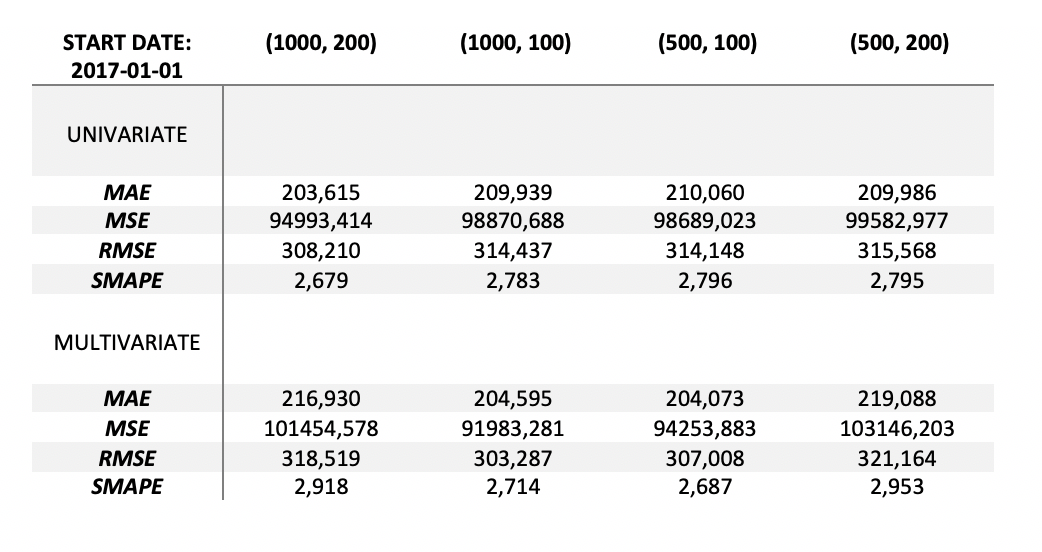
\includegraphics{1_2017.png}
\end{figure} 

\begin{figure}[H]
	\centering
		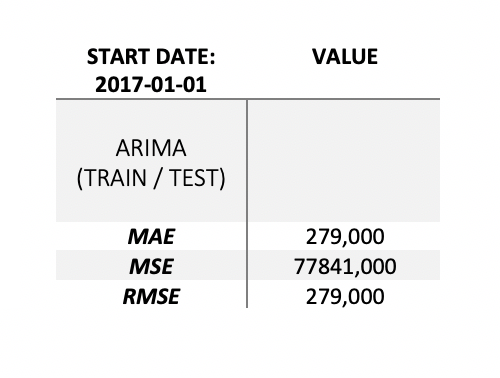
\includegraphics{2_2017.png}
\end{figure} 

\begin{figure}[H]
	\centering
		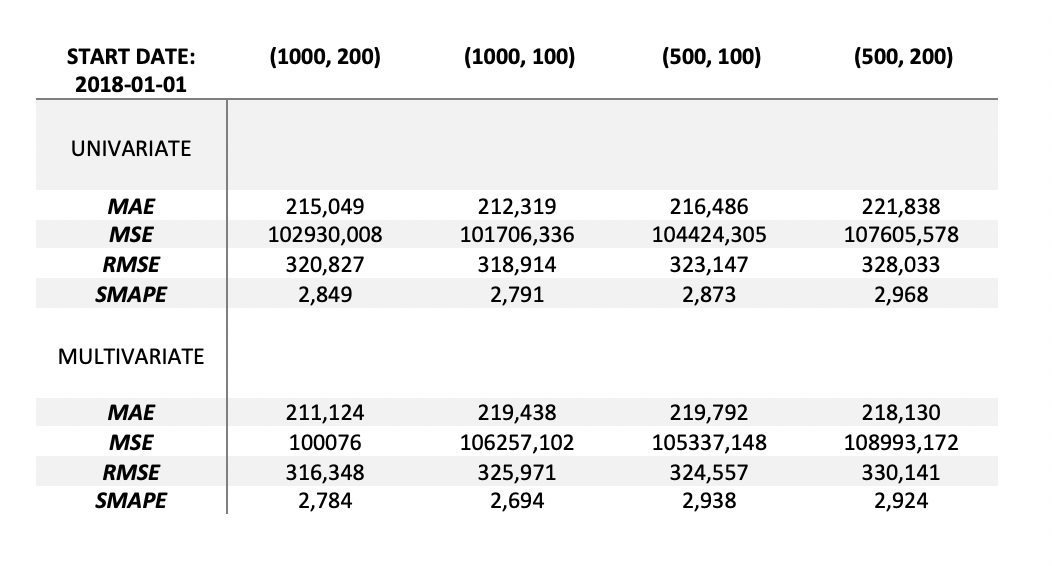
\includegraphics{1_2018.png}
\end{figure} 

\begin{figure}[H]
	\centering
		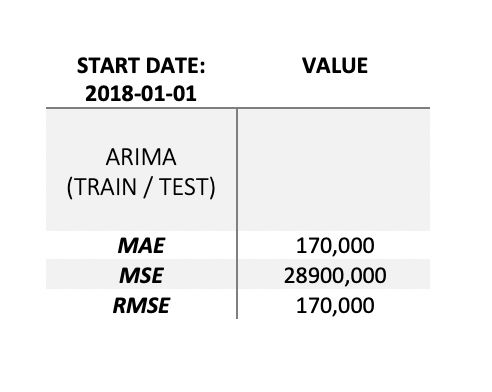
\includegraphics{2_2018.png}
\end{figure} 
    

    

    

    \hypertarget{conclusions}{%
\section{Conclusions}\label{conclusions}}

    Time series are not really different from other machine learning
problems: we want our test set to `look like' our training set, because
we want the model we learned on your training set to still be
appropriate for your test set. That's the important underlying concept
regarding stationarity. Time series have the additional complexity that
there may be long term structure in your data that our model may not be
sophisticated enough to learn.

    Stationarity is an important factor in determining the model structure
for the ARIMA family of models. The reason is because the model has to
have descriptive power over changing conditions, which you have to make
choices to enable. In contrast, an LSTM is not constrained on this
dimension- i.e.~a sufficiently trained LSTM with a sufficient
architectural descriptive base can determine the changing nature of the
time series without the modeler making explicit choices based on that
feature of the data.

    Advantages of ARIMA 1. Simple to implement, no parameter tuning 2.
Easier to handle multivariate data 3. Quick to run

    Advantages of LSTM 1. No pre-requisites (stationarity, no level shifts)
2. Can model non-linear function with neural networks 3. Needs a lot of
data

    ARIMA for instance gives more importance to immediate data points in the
test set and tries to perform well for them but as we get far we see a
larger variance in the predicted output . LSTM works better if we are
dealing with huge amount of data and enough training data is available,
while ARIMA is better for smaller datasets\ldots and our results seem to
confirm this.

    \hypertarget{bitcoin-price-prediction-using-prophet-facebook-with-coinmarketcap-api-optional}{%
\section{Bitcoin Price Prediction using Prophet Facebook with
CoinMarketCap API
(Optional)}\label{bitcoin-price-prediction-using-prophet-facebook-with-coinmarketcap-api-optional}}

    Prophet is a procedure for forecasting time series data based on an
additive model where non-linear trends are fit with yearly, weekly, and
daily seasonality, plus holiday effects. It works best with time series
that have strong seasonal effects and several seasons of historical
data. Prophet is based on decomposable (trend+seasonality+holidays)
models.

    At its core, the Prophet procedure is an~additive regression model~with
four main components: - A piecewise linear or logistic growth curve
trend. Prophet automatically detects changes in trends by selecting
changepoints from the data. - A yearly seasonal component modeled using
Fourier series. - A weekly seasonal component using dummy variables. - A
user-provided list of important holidays.

    In this case we use the CoinMarketCap API, a site of analysis and
monitoring of the cryptocurrency market based in Queens (New York) which
currently provides data on over 2000 cryptocurrencies:

    \begin{Verbatim}[commandchars=\\\{\}]
{\color{incolor}In [{\color{incolor}94}]:} \PY{k}{class} \PY{n+nc}{Predictor}\PY{p}{(}\PY{p}{)}\PY{p}{:}
             \PY{k}{def} \PY{n+nf}{\PYZus{}\PYZus{}init\PYZus{}\PYZus{}}\PY{p}{(}\PY{n+nb+bp}{self}\PY{p}{,} \PY{n}{currency}\PY{p}{,} \PY{n}{training\PYZus{}days}\PY{p}{,} \PY{n}{test\PYZus{}days}\PY{p}{,} \PY{n}{changepoint\PYZus{}prior\PYZus{}scale}\PY{o}{=}\PY{l+m+mi}{1}\PY{p}{)}\PY{p}{:}
                 \PY{n+nb+bp}{self}\PY{o}{.}\PY{n}{currency} \PY{o}{=} \PY{n}{currency}
                 \PY{n+nb+bp}{self}\PY{o}{.}\PY{n}{training\PYZus{}days} \PY{o}{=} \PY{n}{training\PYZus{}days}
                 \PY{n+nb+bp}{self}\PY{o}{.}\PY{n}{test\PYZus{}days} \PY{o}{=} \PY{n}{test\PYZus{}days}
                 \PY{n+nb+bp}{self}\PY{o}{.}\PY{n}{changepoint\PYZus{}prior\PYZus{}scale} \PY{o}{=} \PY{n}{changepoint\PYZus{}prior\PYZus{}scale}
                 \PY{n+nb+bp}{self}\PY{o}{.}\PY{n}{model} \PY{o}{=} \PY{n}{Prophet}\PY{p}{(}\PY{n}{changepoint\PYZus{}prior\PYZus{}scale}\PY{o}{=}\PY{n}{changepoint\PYZus{}prior\PYZus{}scale}\PY{p}{,}
                                      \PY{n}{yearly\PYZus{}seasonality}\PY{o}{=}\PY{k+kc}{False}\PY{p}{,} \PY{n}{daily\PYZus{}seasonality}\PY{o}{=}\PY{k+kc}{False}\PY{p}{)}
                 \PY{k}{assert} \PY{n+nb}{type}\PY{p}{(}\PY{n+nb+bp}{self}\PY{o}{.}\PY{n}{currency}\PY{p}{)} \PY{o}{==} \PY{n+nb}{str}
             
             \PY{k}{def} \PY{n+nf}{\PYZus{}\PYZus{}len\PYZus{}\PYZus{}}\PY{p}{(}\PY{n+nb+bp}{self}\PY{p}{)}\PY{p}{:}
                 \PY{k}{return} \PY{n+nb+bp}{self}\PY{o}{.}\PY{n}{training\PYZus{}days} \PY{o}{+} \PY{n+nb+bp}{self}\PY{o}{.}\PY{n}{test\PYZus{}days}
         
             \PY{k}{def} \PY{n+nf}{make\PYZus{}model}\PY{p}{(}\PY{n+nb+bp}{self}\PY{p}{)}\PY{p}{:}
                 
             \PY{c+c1}{\PYZsh{} Set date ranges to collect training and test data from CoinMarketCap}
                 \PY{n}{test\PYZus{}end} \PY{o}{=} \PY{n}{dt}\PY{o}{.}\PY{n}{today}\PY{p}{(}\PY{p}{)}
                 \PY{n}{test\PYZus{}start} \PY{o}{=} \PY{n}{test\PYZus{}end} \PY{o}{\PYZhy{}} \PY{n}{td}\PY{p}{(}\PY{n}{days}\PY{o}{=}\PY{n+nb+bp}{self}\PY{o}{.}\PY{n}{test\PYZus{}days}\PY{o}{\PYZhy{}}\PY{l+m+mi}{1}\PY{p}{)}
                 \PY{n}{training\PYZus{}end} \PY{o}{=} \PY{n}{test\PYZus{}start} \PY{o}{\PYZhy{}} \PY{n}{td}\PY{p}{(}\PY{n}{days}\PY{o}{=}\PY{l+m+mi}{1}\PY{p}{)}
                 \PY{n}{training\PYZus{}start} \PY{o}{=} \PY{n}{test\PYZus{}start} \PY{o}{\PYZhy{}} \PY{n}{td}\PY{p}{(}\PY{n}{days}\PY{o}{=}\PY{n+nb+bp}{self}\PY{o}{.}\PY{n}{training\PYZus{}days}\PY{p}{)}
         
                 \PY{n}{test\PYZus{}end} \PY{o}{=} \PY{n}{test\PYZus{}end}\PY{o}{.}\PY{n}{strftime}\PY{p}{(}\PY{l+s+s2}{\PYZdq{}}\PY{l+s+s2}{\PYZpc{}}\PY{l+s+s2}{Y}\PY{l+s+s2}{\PYZpc{}}\PY{l+s+s2}{m}\PY{l+s+si}{\PYZpc{}d}\PY{l+s+s2}{\PYZdq{}}\PY{p}{)}
                 \PY{n}{test\PYZus{}start} \PY{o}{=} \PY{n}{test\PYZus{}start}\PY{o}{.}\PY{n}{strftime}\PY{p}{(}\PY{l+s+s2}{\PYZdq{}}\PY{l+s+s2}{\PYZpc{}}\PY{l+s+s2}{Y}\PY{l+s+s2}{\PYZpc{}}\PY{l+s+s2}{m}\PY{l+s+si}{\PYZpc{}d}\PY{l+s+s2}{\PYZdq{}}\PY{p}{)}
                 \PY{n}{training\PYZus{}end} \PY{o}{=} \PY{n}{training\PYZus{}end}\PY{o}{.}\PY{n}{strftime}\PY{p}{(}\PY{l+s+s2}{\PYZdq{}}\PY{l+s+s2}{\PYZpc{}}\PY{l+s+s2}{Y}\PY{l+s+s2}{\PYZpc{}}\PY{l+s+s2}{m}\PY{l+s+si}{\PYZpc{}d}\PY{l+s+s2}{\PYZdq{}}\PY{p}{)}
                 \PY{n}{training\PYZus{}start} \PY{o}{=} \PY{n}{training\PYZus{}start}\PY{o}{.}\PY{n}{strftime}\PY{p}{(}\PY{l+s+s2}{\PYZdq{}}\PY{l+s+s2}{\PYZpc{}}\PY{l+s+s2}{Y}\PY{l+s+s2}{\PYZpc{}}\PY{l+s+s2}{m}\PY{l+s+si}{\PYZpc{}d}\PY{l+s+s2}{\PYZdq{}}\PY{p}{)} 
         
                 \PY{c+c1}{\PYZsh{} Read current price from CMC api}
                 \PY{n}{market\PYZus{}info\PYZus{}for\PYZus{}today} \PY{o}{=} \PY{n}{pd}\PY{o}{.}\PY{n}{read\PYZus{}json}\PY{p}{(}\PY{l+s+s2}{\PYZdq{}}\PY{l+s+s2}{https://api.coinmarketcap.com/v1/ticker/}\PY{l+s+s2}{\PYZdq{}} \PY{o}{+} \PY{n+nb+bp}{self}\PY{o}{.}\PY{n}{currency}\PY{p}{)}
                 \PY{n}{market\PYZus{}info\PYZus{}for\PYZus{}today}\PY{o}{.}\PY{n}{drop}\PY{p}{(}\PY{n}{market\PYZus{}info\PYZus{}for\PYZus{}today}\PY{o}{.}\PY{n}{columns}\PY{p}{[}\PY{p}{[}\PY{l+m+mi}{0}\PY{p}{,} \PY{l+m+mi}{1}\PY{p}{,} \PY{l+m+mi}{2}\PY{p}{,} \PY{l+m+mi}{4}\PY{p}{,} \PY{l+m+mi}{5}\PY{p}{,} \PY{l+m+mi}{6}\PY{p}{,} \PY{l+m+mi}{7}\PY{p}{,} \PY{l+m+mi}{8}\PY{p}{,} \PY{l+m+mi}{9}\PY{p}{,} \PY{l+m+mi}{10}\PY{p}{,} \PY{l+m+mi}{12}\PY{p}{,} \PY{l+m+mi}{13}\PY{p}{,} \PY{l+m+mi}{14}\PY{p}{]}\PY{p}{]}\PY{p}{,}
                                            \PY{n}{axis}\PY{o}{=}\PY{l+m+mi}{1}\PY{p}{,} \PY{n}{inplace}\PY{o}{=}\PY{k+kc}{True}\PY{p}{)}
                 \PY{n}{market\PYZus{}info\PYZus{}for\PYZus{}today}\PY{p}{[}\PY{l+s+s1}{\PYZsq{}}\PY{l+s+s1}{last\PYZus{}updated}\PY{l+s+s1}{\PYZsq{}}\PY{p}{]} \PY{o}{=} \PY{n}{market\PYZus{}info\PYZus{}for\PYZus{}today}\PY{p}{[}\PY{l+s+s1}{\PYZsq{}}\PY{l+s+s1}{last\PYZus{}updated}\PY{l+s+s1}{\PYZsq{}}\PY{p}{]}\PY{o}{.}\PY{n}{apply}\PY{p}{(}\PY{k}{lambda} \PY{n}{x}\PY{p}{:} \PY{n}{dt}\PY{o}{.}\PY{n}{fromtimestamp}\PY{p}{(}\PY{n+nb}{int}\PY{p}{(}\PY{n}{x}\PY{p}{)}\PY{p}{)}\PY{p}{)}
                 \PY{n}{market\PYZus{}info\PYZus{}for\PYZus{}today}\PY{o}{.}\PY{n}{columns} \PY{o}{=} \PY{p}{[}\PY{l+s+s1}{\PYZsq{}}\PY{l+s+s1}{ds}\PY{l+s+s1}{\PYZsq{}}\PY{p}{,} \PY{l+s+s1}{\PYZsq{}}\PY{l+s+s1}{y}\PY{l+s+s1}{\PYZsq{}}\PY{p}{]}
                 
                 \PY{c+c1}{\PYZsh{} Read table from historical data page of cryptocurrency}
                 \PY{k}{if} \PY{n+nb+bp}{self}\PY{o}{.}\PY{n}{test\PYZus{}days} \PY{o}{\PYZgt{}} \PY{l+m+mi}{1}\PY{p}{:}
                     \PY{n}{market\PYZus{}info\PYZus{}test} \PY{o}{=} \PY{n}{pd}\PY{o}{.}\PY{n}{read\PYZus{}html}\PY{p}{(}\PY{l+s+s2}{\PYZdq{}}\PY{l+s+s2}{https://coinmarketcap.com/currencies/}\PY{l+s+s2}{\PYZdq{}} 
                                                     \PY{o}{+} \PY{n+nb+bp}{self}\PY{o}{.}\PY{n}{currency} \PY{o}{+} \PY{l+s+s2}{\PYZdq{}}\PY{l+s+s2}{/historical\PYZhy{}data/?start=}\PY{l+s+s2}{\PYZdq{}} 
                                                     \PY{o}{+} \PY{n}{test\PYZus{}start} \PY{o}{+} \PY{l+s+s2}{\PYZdq{}}\PY{l+s+s2}{\PYZam{}end=}\PY{l+s+s2}{\PYZdq{}} \PY{o}{+} \PY{n}{test\PYZus{}end}\PY{p}{)}\PY{p}{[}\PY{l+m+mi}{0}\PY{p}{]}
                     \PY{n}{market\PYZus{}info\PYZus{}test}\PY{o}{.}\PY{n}{drop}\PY{p}{(}\PY{n}{market\PYZus{}info\PYZus{}test}\PY{o}{.}\PY{n}{columns}\PY{p}{[}\PY{p}{[}\PY{l+m+mi}{1}\PY{p}{,} \PY{l+m+mi}{2}\PY{p}{,} \PY{l+m+mi}{3}\PY{p}{,} \PY{l+m+mi}{5}\PY{p}{,} \PY{l+m+mi}{6}\PY{p}{]}\PY{p}{]}\PY{p}{,} \PY{n}{axis}\PY{o}{=}\PY{l+m+mi}{1}\PY{p}{,} \PY{n}{inplace}\PY{o}{=}\PY{k+kc}{True}\PY{p}{)}
                     \PY{n}{market\PYZus{}info\PYZus{}test} \PY{o}{=} \PY{n}{market\PYZus{}info\PYZus{}test}\PY{o}{.}\PY{n}{assign}\PY{p}{(}\PY{n}{Date}\PY{o}{=}\PY{n}{pd}\PY{o}{.}\PY{n}{to\PYZus{}datetime}\PY{p}{(}\PY{n}{market\PYZus{}info\PYZus{}test}\PY{p}{[}\PY{l+s+s1}{\PYZsq{}}\PY{l+s+s1}{Date}\PY{l+s+s1}{\PYZsq{}}\PY{p}{]}\PY{p}{)}\PY{p}{)}
                     \PY{n}{market\PYZus{}info\PYZus{}test}\PY{o}{.}\PY{n}{iloc}\PY{p}{[}\PY{p}{:}\PY{p}{:}\PY{o}{\PYZhy{}}\PY{l+m+mi}{1}\PY{p}{]}\PY{o}{.}\PY{n}{sort\PYZus{}index}\PY{p}{(}\PY{n}{axis}\PY{o}{=}\PY{l+m+mi}{0} \PY{p}{,}\PY{n}{ascending}\PY{o}{=}\PY{k+kc}{False}\PY{p}{)}
                     \PY{n}{market\PYZus{}info\PYZus{}test}\PY{o}{.}\PY{n}{columns} \PY{o}{=} \PY{p}{[}\PY{l+s+s1}{\PYZsq{}}\PY{l+s+s1}{ds}\PY{l+s+s1}{\PYZsq{}}\PY{p}{,} \PY{l+s+s1}{\PYZsq{}}\PY{l+s+s1}{y}\PY{l+s+s1}{\PYZsq{}}\PY{p}{]}
                     \PY{n}{market\PYZus{}info\PYZus{}test} \PY{o}{=} \PY{n}{pd}\PY{o}{.}\PY{n}{concat}\PY{p}{(}\PY{p}{[}\PY{n}{market\PYZus{}info\PYZus{}for\PYZus{}today}\PY{p}{,} \PY{n}{market\PYZus{}info\PYZus{}test}\PY{p}{]}\PY{p}{,} \PY{n}{axis}\PY{o}{=}\PY{l+m+mi}{0}\PY{p}{,} \PY{n}{ignore\PYZus{}index}\PY{o}{=}\PY{k+kc}{True}\PY{p}{)}
                 \PY{k}{else}\PY{p}{:}
                     \PY{n}{market\PYZus{}info\PYZus{}test} \PY{o}{=} \PY{n}{market\PYZus{}info\PYZus{}for\PYZus{}today}
                 
                 \PY{n}{market\PYZus{}info\PYZus{}test}\PY{p}{[}\PY{l+s+s1}{\PYZsq{}}\PY{l+s+s1}{y}\PY{l+s+s1}{\PYZsq{}}\PY{p}{]} \PY{o}{=} \PY{n}{np}\PY{o}{.}\PY{n}{log}\PY{p}{(}\PY{n}{market\PYZus{}info\PYZus{}test}\PY{p}{[}\PY{l+s+s1}{\PYZsq{}}\PY{l+s+s1}{y}\PY{l+s+s1}{\PYZsq{}}\PY{p}{]}\PY{p}{)}
                 \PY{n+nb+bp}{self}\PY{o}{.}\PY{n}{test} \PY{o}{=} \PY{n}{market\PYZus{}info\PYZus{}test}\PY{o}{.}\PY{n}{iloc}\PY{p}{[}\PY{p}{:}\PY{p}{:}\PY{o}{\PYZhy{}}\PY{l+m+mi}{1}\PY{p}{]}\PY{o}{.}\PY{n}{sort\PYZus{}index}\PY{p}{(}\PY{n}{axis}\PY{o}{=}\PY{l+m+mi}{0} \PY{p}{,}\PY{n}{ascending}\PY{o}{=}\PY{k+kc}{False}\PY{p}{)}
         
                 \PY{n}{market\PYZus{}info\PYZus{}training} \PY{o}{=} \PY{n}{pd}\PY{o}{.}\PY{n}{read\PYZus{}html}\PY{p}{(}\PY{l+s+s2}{\PYZdq{}}\PY{l+s+s2}{https://coinmarketcap.com/currencies/}\PY{l+s+s2}{\PYZdq{}} 
                                                     \PY{o}{+} \PY{n+nb+bp}{self}\PY{o}{.}\PY{n}{currency} \PY{o}{+} \PY{l+s+s2}{\PYZdq{}}\PY{l+s+s2}{/historical\PYZhy{}data/?start=}\PY{l+s+s2}{\PYZdq{}} 
                                                     \PY{o}{+} \PY{n}{training\PYZus{}start} \PY{o}{+} \PY{l+s+s2}{\PYZdq{}}\PY{l+s+s2}{\PYZam{}end=}\PY{l+s+s2}{\PYZdq{}} \PY{o}{+} \PY{n}{training\PYZus{}end}\PY{p}{)}\PY{p}{[}\PY{l+m+mi}{0}\PY{p}{]}
                 \PY{n}{market\PYZus{}info\PYZus{}training}\PY{o}{.}\PY{n}{drop}\PY{p}{(}\PY{n}{market\PYZus{}info\PYZus{}training}\PY{o}{.}\PY{n}{columns}\PY{p}{[}\PY{p}{[}\PY{l+m+mi}{1}\PY{p}{,} \PY{l+m+mi}{2}\PY{p}{,} \PY{l+m+mi}{3}\PY{p}{,} \PY{l+m+mi}{5}\PY{p}{,} \PY{l+m+mi}{6}\PY{p}{]}\PY{p}{]}\PY{p}{,} \PY{n}{axis}\PY{o}{=}\PY{l+m+mi}{1}\PY{p}{,} \PY{n}{inplace}\PY{o}{=}\PY{k+kc}{True}\PY{p}{)}
                 \PY{n}{market\PYZus{}info\PYZus{}training} \PY{o}{=} \PY{n}{market\PYZus{}info\PYZus{}training}\PY{o}{.}\PY{n}{assign}\PY{p}{(}\PY{n}{Date}\PY{o}{=}\PY{n}{pd}\PY{o}{.}\PY{n}{to\PYZus{}datetime}\PY{p}{(}\PY{n}{market\PYZus{}info\PYZus{}training}\PY{p}{[}\PY{l+s+s1}{\PYZsq{}}\PY{l+s+s1}{Date}\PY{l+s+s1}{\PYZsq{}}\PY{p}{]}\PY{p}{)}\PY{p}{)}
                 \PY{n}{market\PYZus{}info\PYZus{}training}\PY{o}{.}\PY{n}{columns} \PY{o}{=} \PY{p}{[}\PY{l+s+s1}{\PYZsq{}}\PY{l+s+s1}{ds}\PY{l+s+s1}{\PYZsq{}}\PY{p}{,} \PY{l+s+s1}{\PYZsq{}}\PY{l+s+s1}{y}\PY{l+s+s1}{\PYZsq{}}\PY{p}{]}
                 \PY{n}{market\PYZus{}info\PYZus{}training}\PY{p}{[}\PY{l+s+s1}{\PYZsq{}}\PY{l+s+s1}{y}\PY{l+s+s1}{\PYZsq{}}\PY{p}{]} \PY{o}{=} \PY{n}{np}\PY{o}{.}\PY{n}{log}\PY{p}{(}\PY{n}{market\PYZus{}info\PYZus{}training}\PY{p}{[}\PY{l+s+s1}{\PYZsq{}}\PY{l+s+s1}{y}\PY{l+s+s1}{\PYZsq{}}\PY{p}{]}\PY{p}{)}
                 \PY{n+nb+bp}{self}\PY{o}{.}\PY{n}{training} \PY{o}{=} \PY{n}{market\PYZus{}info\PYZus{}training}\PY{o}{.}\PY{n}{iloc}\PY{p}{[}\PY{p}{:}\PY{p}{:}\PY{o}{\PYZhy{}}\PY{l+m+mi}{1}\PY{p}{]}\PY{o}{.}\PY{n}{sort\PYZus{}index}\PY{p}{(}\PY{n}{axis}\PY{o}{=}\PY{l+m+mi}{0} \PY{p}{,}\PY{n}{ascending}\PY{o}{=}\PY{k+kc}{False}\PY{p}{)}
                 
                 
                 \PY{c+c1}{\PYZsh{} Fit training data to model and eval speed}
                 \PY{n+nb}{print}\PY{p}{(}\PY{l+s+s2}{\PYZdq{}}\PY{l+s+s2}{Fitting training data...}\PY{l+s+s2}{\PYZdq{}}\PY{p}{)}
                 \PY{n}{start} \PY{o}{=} \PY{n}{time}\PY{o}{.}\PY{n}{time}\PY{p}{(}\PY{p}{)}
                 \PY{n+nb+bp}{self}\PY{o}{.}\PY{n}{model}\PY{o}{.}\PY{n}{fit}\PY{p}{(}\PY{n+nb+bp}{self}\PY{o}{.}\PY{n}{training}\PY{p}{)}
                 \PY{n+nb}{print}\PY{p}{(}\PY{l+s+s2}{\PYZdq{}}\PY{l+s+s2}{Took}\PY{l+s+s2}{\PYZdq{}}\PY{p}{,} \PY{n+nb}{round}\PY{p}{(}\PY{n}{time}\PY{o}{.}\PY{n}{time}\PY{p}{(}\PY{p}{)}\PY{o}{\PYZhy{}}\PY{n}{start}\PY{p}{,} \PY{l+m+mi}{4}\PY{p}{)}\PY{p}{,} \PY{l+s+s2}{\PYZdq{}}\PY{l+s+s2}{seconds.}\PY{l+s+s2}{\PYZdq{}}\PY{p}{,} \PY{l+s+s2}{\PYZdq{}}\PY{l+s+se}{\PYZbs{}n}\PY{l+s+s2}{\PYZdq{}}\PY{p}{)}
                 
                 
                 \PY{c+c1}{\PYZsh{} Evaluate model by calculating Mean Absolute Error of predictions }
                 \PY{c+c1}{\PYZsh{} for test days with actual prices on those days}
                 \PY{n+nb}{print}\PY{p}{(}\PY{l+s+s2}{\PYZdq{}}\PY{l+s+s2}{Evaluating model on testing data...}\PY{l+s+s2}{\PYZdq{}}\PY{p}{)}
                 \PY{n}{future} \PY{o}{=} \PY{n+nb+bp}{self}\PY{o}{.}\PY{n}{model}\PY{o}{.}\PY{n}{make\PYZus{}future\PYZus{}dataframe}\PY{p}{(}\PY{n}{periods}\PY{o}{=}\PY{n+nb+bp}{self}\PY{o}{.}\PY{n}{test\PYZus{}days}\PY{p}{)}
                 \PY{n}{forecast} \PY{o}{=} \PY{n+nb+bp}{self}\PY{o}{.}\PY{n}{model}\PY{o}{.}\PY{n}{predict}\PY{p}{(}\PY{n}{future}\PY{p}{)}
                 \PY{n}{forecast} \PY{o}{=} \PY{n}{forecast}\PY{p}{[}\PY{o}{\PYZhy{}}\PY{n+nb+bp}{self}\PY{o}{.}\PY{n}{test\PYZus{}days}\PY{p}{:}\PY{p}{]}
                 
                 \PY{n}{revert} \PY{o}{=} \PY{k}{lambda} \PY{n}{x}\PY{p}{:} \PY{n}{np}\PY{o}{.}\PY{n}{e}\PY{o}{*}\PY{o}{*}\PY{n}{x}
                 \PY{n}{forecast}\PY{p}{[}\PY{l+s+s1}{\PYZsq{}}\PY{l+s+s1}{yhat}\PY{l+s+s1}{\PYZsq{}}\PY{p}{]} \PY{o}{=} \PY{n}{forecast}\PY{p}{[}\PY{l+s+s1}{\PYZsq{}}\PY{l+s+s1}{yhat}\PY{l+s+s1}{\PYZsq{}}\PY{p}{]}\PY{o}{.}\PY{n}{apply}\PY{p}{(}\PY{n}{revert}\PY{p}{)}
                 \PY{n}{forecast}\PY{p}{[}\PY{l+s+s1}{\PYZsq{}}\PY{l+s+s1}{yhat\PYZus{}upper}\PY{l+s+s1}{\PYZsq{}}\PY{p}{]} \PY{o}{=} \PY{n}{forecast}\PY{p}{[}\PY{l+s+s1}{\PYZsq{}}\PY{l+s+s1}{yhat\PYZus{}upper}\PY{l+s+s1}{\PYZsq{}}\PY{p}{]}\PY{o}{.}\PY{n}{apply}\PY{p}{(}\PY{n}{revert}\PY{p}{)}
                 \PY{n}{forecast}\PY{p}{[}\PY{l+s+s1}{\PYZsq{}}\PY{l+s+s1}{yhat\PYZus{}lower}\PY{l+s+s1}{\PYZsq{}}\PY{p}{]} \PY{o}{=} \PY{n}{forecast}\PY{p}{[}\PY{l+s+s1}{\PYZsq{}}\PY{l+s+s1}{yhat\PYZus{}lower}\PY{l+s+s1}{\PYZsq{}}\PY{p}{]}\PY{o}{.}\PY{n}{apply}\PY{p}{(}\PY{n}{revert}\PY{p}{)}
                 \PY{n+nb+bp}{self}\PY{o}{.}\PY{n}{error\PYZus{}forecast} \PY{o}{=} \PY{n}{forecast}\PY{p}{[}\PY{p}{[}\PY{l+s+s1}{\PYZsq{}}\PY{l+s+s1}{ds}\PY{l+s+s1}{\PYZsq{}}\PY{p}{,} \PY{l+s+s1}{\PYZsq{}}\PY{l+s+s1}{yhat}\PY{l+s+s1}{\PYZsq{}}\PY{p}{,} \PY{l+s+s1}{\PYZsq{}}\PY{l+s+s1}{yhat\PYZus{}upper}\PY{l+s+s1}{\PYZsq{}}\PY{p}{,} \PY{l+s+s1}{\PYZsq{}}\PY{l+s+s1}{yhat\PYZus{}lower}\PY{l+s+s1}{\PYZsq{}}\PY{p}{]}\PY{p}{]}
                 \PY{n}{test} \PY{o}{=} \PY{n+nb+bp}{self}\PY{o}{.}\PY{n}{test}\PY{o}{.}\PY{n}{copy}\PY{p}{(}\PY{n}{deep}\PY{o}{=}\PY{k+kc}{True}\PY{p}{)}\PY{p}{[}\PY{l+s+s1}{\PYZsq{}}\PY{l+s+s1}{y}\PY{l+s+s1}{\PYZsq{}}\PY{p}{]}\PY{o}{.}\PY{n}{apply}\PY{p}{(}\PY{n}{revert}\PY{p}{)}
                 
                 \PY{k}{if} \PY{o+ow}{not} \PY{n+nb}{all}\PY{p}{(}\PY{p}{[}\PY{n}{x}\PY{o}{.}\PY{n}{date}\PY{p}{(}\PY{p}{)}\PY{o}{==}\PY{n}{y}\PY{o}{.}\PY{n}{date}\PY{p}{(}\PY{p}{)} \PY{k}{for} \PY{n}{x}\PY{p}{,} \PY{n}{y} \PY{o+ow}{in} \PY{n+nb}{zip}\PY{p}{(}\PY{n}{forecast}\PY{p}{[}\PY{l+s+s1}{\PYZsq{}}\PY{l+s+s1}{ds}\PY{l+s+s1}{\PYZsq{}}\PY{p}{]}\PY{p}{,} \PY{n+nb+bp}{self}\PY{o}{.}\PY{n}{test}\PY{p}{[}\PY{l+s+s1}{\PYZsq{}}\PY{l+s+s1}{ds}\PY{l+s+s1}{\PYZsq{}}\PY{p}{]}\PY{p}{)}\PY{p}{]}\PY{p}{)}\PY{p}{:}
                     \PY{k}{raise} \PY{n+ne}{ValueError}\PY{p}{(}\PY{l+s+s2}{\PYZdq{}}\PY{l+s+s2}{Test or Forecast Dataframe isn}\PY{l+s+s2}{\PYZsq{}}\PY{l+s+s2}{t ordered by date or order is mismatched}\PY{l+s+s2}{\PYZdq{}}\PY{p}{)}
                 \PY{n+nb+bp}{self}\PY{o}{.}\PY{n}{mae\PYZus{}upper} \PY{o}{=} \PY{n+nb}{sum}\PY{p}{(}\PY{p}{[}\PY{n+nb}{abs}\PY{p}{(}\PY{n}{yhat} \PY{o}{\PYZhy{}} \PY{n}{y}\PY{p}{)} \PY{k}{for} \PY{n}{yhat}\PY{p}{,} \PY{n}{y} \PY{o+ow}{in} \PY{n+nb}{zip}\PY{p}{(}\PY{n}{forecast}\PY{p}{[}\PY{l+s+s1}{\PYZsq{}}\PY{l+s+s1}{yhat\PYZus{}upper}\PY{l+s+s1}{\PYZsq{}}\PY{p}{]}\PY{p}{,} 
                                                                        \PY{n}{test}\PY{p}{)}\PY{p}{]}\PY{p}{)} \PY{o}{/} \PY{n+nb}{len}\PY{p}{(}\PY{n}{forecast}\PY{p}{)}
                 \PY{n+nb+bp}{self}\PY{o}{.}\PY{n}{mae} \PY{o}{=} \PY{n+nb}{sum}\PY{p}{(}\PY{p}{[}\PY{n+nb}{abs}\PY{p}{(}\PY{n}{yhat} \PY{o}{\PYZhy{}} \PY{n}{y}\PY{p}{)} \PY{k}{for} \PY{n}{yhat}\PY{p}{,} \PY{n}{y} \PY{o+ow}{in} \PY{n+nb}{zip}\PY{p}{(}\PY{n}{forecast}\PY{p}{[}\PY{l+s+s1}{\PYZsq{}}\PY{l+s+s1}{yhat}\PY{l+s+s1}{\PYZsq{}}\PY{p}{]}\PY{p}{,} \PY{n}{test}\PY{p}{)}\PY{p}{]}\PY{p}{)} \PY{o}{/} \PY{n+nb}{len}\PY{p}{(}\PY{n}{forecast}\PY{p}{)}
                 \PY{n+nb+bp}{self}\PY{o}{.}\PY{n}{mae\PYZus{}lower} \PY{o}{=} \PY{n+nb}{sum}\PY{p}{(}\PY{p}{[}\PY{n+nb}{abs}\PY{p}{(}\PY{n}{yhat} \PY{o}{\PYZhy{}} \PY{n}{y}\PY{p}{)} \PY{k}{for} \PY{n}{yhat}\PY{p}{,} \PY{n}{y} \PY{o+ow}{in} \PY{n+nb}{zip}\PY{p}{(}\PY{n}{forecast}\PY{p}{[}\PY{l+s+s1}{\PYZsq{}}\PY{l+s+s1}{yhat\PYZus{}lower}\PY{l+s+s1}{\PYZsq{}}\PY{p}{]}\PY{p}{,} 
                                                                        \PY{n}{test}\PY{p}{)}\PY{p}{]}\PY{p}{)} \PY{o}{/} \PY{n+nb}{len}\PY{p}{(}\PY{n}{forecast}\PY{p}{)}
                 \PY{n+nb}{print}\PY{p}{(}\PY{l+s+s2}{\PYZdq{}}\PY{l+s+s2}{Upper MAE: \PYZdl{}}\PY{l+s+s2}{\PYZdq{}} \PY{o}{+} \PY{n+nb}{str}\PY{p}{(}\PY{n+nb+bp}{self}\PY{o}{.}\PY{n}{mae\PYZus{}upper}\PY{p}{)}\PY{p}{)}
                 \PY{n+nb}{print}\PY{p}{(}\PY{l+s+s2}{\PYZdq{}}\PY{l+s+s2}{MAE: \PYZdl{}}\PY{l+s+s2}{\PYZdq{}} \PY{o}{+} \PY{n+nb}{str}\PY{p}{(}\PY{n+nb+bp}{self}\PY{o}{.}\PY{n}{mae}\PY{p}{)}\PY{p}{)}
                 \PY{n+nb}{print}\PY{p}{(}\PY{l+s+s2}{\PYZdq{}}\PY{l+s+s2}{Lower MAE: \PYZdl{}}\PY{l+s+s2}{\PYZdq{}} \PY{o}{+} \PY{n+nb}{str}\PY{p}{(}\PY{n+nb+bp}{self}\PY{o}{.}\PY{n}{mae\PYZus{}lower}\PY{p}{)} \PY{o}{+} \PY{l+s+s2}{\PYZdq{}}\PY{l+s+se}{\PYZbs{}n}\PY{l+s+s2}{\PYZdq{}}\PY{p}{)}
             
             \PY{k}{def} \PY{n+nf}{predict}\PY{p}{(}\PY{n+nb+bp}{self}\PY{p}{,} \PY{n}{days}\PY{o}{=}\PY{l+m+mi}{30}\PY{p}{,} \PY{n}{make\PYZus{}plot}\PY{o}{=}\PY{k+kc}{True}\PY{p}{)}\PY{p}{:}
                 \PY{c+c1}{\PYZsh{} Reinitialize model and fit both training and test }
                 \PY{c+c1}{\PYZsh{} data to create most up\PYZhy{}to\PYZhy{}date model}
                 \PY{n+nb+bp}{self}\PY{o}{.}\PY{n}{model} \PY{o}{=} \PY{n}{Prophet}\PY{p}{(}\PY{n}{changepoint\PYZus{}prior\PYZus{}scale}\PY{o}{=}\PY{n+nb+bp}{self}\PY{o}{.}\PY{n}{changepoint\PYZus{}prior\PYZus{}scale}\PY{p}{,} 
                                      \PY{n}{yearly\PYZus{}seasonality}\PY{o}{=}\PY{k+kc}{False}\PY{p}{,} \PY{n}{daily\PYZus{}seasonality}\PY{o}{=}\PY{k+kc}{False}\PY{p}{)}
                 \PY{n+nb}{print}\PY{p}{(}\PY{l+s+s2}{\PYZdq{}}\PY{l+s+s2}{Fitting all data...}\PY{l+s+s2}{\PYZdq{}}\PY{p}{)}
                 \PY{n}{start} \PY{o}{=} \PY{n}{time}\PY{o}{.}\PY{n}{time}\PY{p}{(}\PY{p}{)}
                 \PY{n+nb+bp}{self}\PY{o}{.}\PY{n}{model}\PY{o}{.}\PY{n}{fit}\PY{p}{(}\PY{n}{pd}\PY{o}{.}\PY{n}{concat}\PY{p}{(}\PY{p}{[}\PY{n+nb+bp}{self}\PY{o}{.}\PY{n}{test}\PY{p}{,} \PY{n+nb+bp}{self}\PY{o}{.}\PY{n}{training}\PY{p}{]}\PY{p}{)}\PY{p}{)}
                 \PY{n+nb}{print}\PY{p}{(}\PY{l+s+s2}{\PYZdq{}}\PY{l+s+s2}{Took}\PY{l+s+s2}{\PYZdq{}}\PY{p}{,} \PY{n+nb}{round}\PY{p}{(}\PY{n}{time}\PY{o}{.}\PY{n}{time}\PY{p}{(}\PY{p}{)}\PY{o}{\PYZhy{}}\PY{n}{start}\PY{p}{,} \PY{l+m+mi}{3}\PY{p}{)}\PY{p}{,} \PY{l+s+s2}{\PYZdq{}}\PY{l+s+s2}{seconds.}\PY{l+s+s2}{\PYZdq{}}\PY{p}{)}
                 
                 \PY{n}{future} \PY{o}{=} \PY{n+nb+bp}{self}\PY{o}{.}\PY{n}{model}\PY{o}{.}\PY{n}{make\PYZus{}future\PYZus{}dataframe}\PY{p}{(}\PY{n}{periods}\PY{o}{=}\PY{n}{days}\PY{p}{)}
                 \PY{n+nb+bp}{self}\PY{o}{.}\PY{n}{forecast} \PY{o}{=} \PY{n+nb+bp}{self}\PY{o}{.}\PY{n}{model}\PY{o}{.}\PY{n}{predict}\PY{p}{(}\PY{n}{future}\PY{p}{)}
                 
                 \PY{n}{revert} \PY{o}{=} \PY{k}{lambda} \PY{n}{x}\PY{p}{:} \PY{n}{np}\PY{o}{.}\PY{n}{e}\PY{o}{*}\PY{o}{*}\PY{n}{x}
                 \PY{n+nb+bp}{self}\PY{o}{.}\PY{n}{model}\PY{o}{.}\PY{n}{history}\PY{p}{[}\PY{l+s+s1}{\PYZsq{}}\PY{l+s+s1}{y}\PY{l+s+s1}{\PYZsq{}}\PY{p}{]} \PY{o}{=} \PY{n+nb+bp}{self}\PY{o}{.}\PY{n}{model}\PY{o}{.}\PY{n}{history}\PY{p}{[}\PY{l+s+s1}{\PYZsq{}}\PY{l+s+s1}{y}\PY{l+s+s1}{\PYZsq{}}\PY{p}{]}\PY{o}{.}\PY{n}{apply}\PY{p}{(}\PY{n}{revert}\PY{p}{)}
                 \PY{n+nb+bp}{self}\PY{o}{.}\PY{n}{forecast}\PY{p}{[}\PY{l+s+s1}{\PYZsq{}}\PY{l+s+s1}{yhat}\PY{l+s+s1}{\PYZsq{}}\PY{p}{]} \PY{o}{=} \PY{n+nb+bp}{self}\PY{o}{.}\PY{n}{forecast}\PY{p}{[}\PY{l+s+s1}{\PYZsq{}}\PY{l+s+s1}{yhat}\PY{l+s+s1}{\PYZsq{}}\PY{p}{]}\PY{o}{.}\PY{n}{apply}\PY{p}{(}\PY{n}{revert}\PY{p}{)}
                 \PY{n+nb+bp}{self}\PY{o}{.}\PY{n}{forecast}\PY{p}{[}\PY{l+s+s1}{\PYZsq{}}\PY{l+s+s1}{yhat\PYZus{}upper}\PY{l+s+s1}{\PYZsq{}}\PY{p}{]} \PY{o}{=} \PY{n+nb+bp}{self}\PY{o}{.}\PY{n}{forecast}\PY{p}{[}\PY{l+s+s1}{\PYZsq{}}\PY{l+s+s1}{yhat\PYZus{}upper}\PY{l+s+s1}{\PYZsq{}}\PY{p}{]}\PY{o}{.}\PY{n}{apply}\PY{p}{(}\PY{n}{revert}\PY{p}{)}
                 \PY{n+nb+bp}{self}\PY{o}{.}\PY{n}{forecast}\PY{p}{[}\PY{l+s+s1}{\PYZsq{}}\PY{l+s+s1}{yhat\PYZus{}lower}\PY{l+s+s1}{\PYZsq{}}\PY{p}{]} \PY{o}{=} \PY{n+nb+bp}{self}\PY{o}{.}\PY{n}{forecast}\PY{p}{[}\PY{l+s+s1}{\PYZsq{}}\PY{l+s+s1}{yhat\PYZus{}lower}\PY{l+s+s1}{\PYZsq{}}\PY{p}{]}\PY{o}{.}\PY{n}{apply}\PY{p}{(}\PY{n}{revert}\PY{p}{)}
                 
                 \PY{c+c1}{\PYZsh{} Plot forecast and actual data if plotting desired}
                 \PY{k}{if} \PY{n}{make\PYZus{}plot}\PY{p}{:} \PY{k}{return} \PY{n+nb+bp}{self}\PY{o}{.}\PY{n}{model}\PY{o}{.}\PY{n}{plot}\PY{p}{(}\PY{n+nb+bp}{self}\PY{o}{.}\PY{n}{forecast}\PY{p}{)}\PY{p}{,} \PY{n+nb+bp}{self}\PY{o}{.}\PY{n}{model}\PY{o}{.}\PY{n}{plot\PYZus{}components}\PY{p}{(}\PY{n+nb+bp}{self}\PY{o}{.}\PY{n}{forecast}\PY{p}{)}
\end{Verbatim}

    We use 150 training days and 3 test days. The testing period is short
because thats the max range of days that the model is accurate enough
for. As such, this model should not be used for long forecasting of
prices and should only be used for finding short-term prices or the
long-term trend (up or down).

    \begin{Verbatim}[commandchars=\\\{\}]
{\color{incolor}In [{\color{incolor}95}]:} \PY{n}{bitcoin\PYZus{}predictor} \PY{o}{=} \PY{n}{Predictor}\PY{p}{(}\PY{l+s+s2}{\PYZdq{}}\PY{l+s+s2}{bitcoin}\PY{l+s+s2}{\PYZdq{}}\PY{p}{,} \PY{l+m+mi}{150}\PY{p}{,} \PY{l+m+mi}{3}\PY{p}{)}
\end{Verbatim}

    We assemble model:

    \begin{Verbatim}[commandchars=\\\{\}]
{\color{incolor}In [{\color{incolor}96}]:} \PY{n}{bitcoin\PYZus{}predictor}\PY{o}{.}\PY{n}{make\PYZus{}model}\PY{p}{(}\PY{p}{)}
\end{Verbatim}

    \begin{Verbatim}[commandchars=\\\{\}]
Fitting training data{\ldots}
Took 0.1363 seconds. 

Evaluating model on testing data{\ldots}
Upper MAE: \$1328.3178726991143
MAE: \$629.2084667897161
Lower MAE: \$52.30876775269159


    \end{Verbatim}

    We expect the next 15 days of the price value:

    \begin{Verbatim}[commandchars=\\\{\}]
{\color{incolor}In [{\color{incolor}97}]:} \PY{n}{bitcoin\PYZus{}predictor}\PY{o}{.}\PY{n}{predict}\PY{p}{(}\PY{l+m+mi}{15}\PY{p}{)}
         \PY{n}{plt}\PY{o}{.}\PY{n}{show}\PY{p}{(}\PY{p}{)}
\end{Verbatim}

    \begin{Verbatim}[commandchars=\\\{\}]
Fitting all data{\ldots}
Took 0.208 seconds.

    \end{Verbatim}

    \begin{center}
    \adjustimage{max size={0.9\linewidth}{0.9\paperheight}}{output_276_1.png}
    \end{center}
    { \hspace*{\fill} \\}
    
    \begin{center}
    \adjustimage{max size={0.9\linewidth}{0.9\paperheight}}{output_276_2.png}
    \end{center}
    { \hspace*{\fill} \\}
    
    The forecast for testing period is:

    \begin{Verbatim}[commandchars=\\\{\}]
{\color{incolor}In [{\color{incolor}98}]:} \PY{n}{bitcoin\PYZus{}predictor}\PY{o}{.}\PY{n}{error\PYZus{}forecast}\PY{o}{.}\PY{n}{head}\PY{p}{(}\PY{p}{)}
\end{Verbatim}

\begin{Verbatim}[commandchars=\\\{\}]
{\color{outcolor}Out[{\color{outcolor}98}]:}             ds          yhat    yhat\_upper    yhat\_lower
         150 2019-07-20  11318.450036  11985.766504  10700.116753
         151 2019-07-21  11205.940881  11899.499359  10551.374273
         152 2019-07-22  11254.896599  11991.349872  10567.579445
\end{Verbatim}
            
    The actual value(s) for testing period is:

    \begin{Verbatim}[commandchars=\\\{\}]
{\color{incolor}In [{\color{incolor}99}]:} \PY{n}{bitcoin\PYZus{}predictor}\PY{o}{.}\PY{n}{test}\PY{p}{[}\PY{l+s+s1}{\PYZsq{}}\PY{l+s+s1}{y}\PY{l+s+s1}{\PYZsq{}}\PY{p}{]} \PY{o}{=} \PY{n}{bitcoin\PYZus{}predictor}\PY{o}{.}\PY{n}{test}\PY{p}{[}\PY{l+s+s1}{\PYZsq{}}\PY{l+s+s1}{y}\PY{l+s+s1}{\PYZsq{}}\PY{p}{]}\PY{o}{.}\PY{n}{apply}\PY{p}{(}\PY{k}{lambda} \PY{n}{x}\PY{p}{:} \PY{n}{np}\PY{o}{.}\PY{n}{e}\PY{o}{*}\PY{o}{*}\PY{n}{x}\PY{p}{)}
         \PY{n}{bitcoin\PYZus{}predictor}\PY{o}{.}\PY{n}{test}\PY{o}{.}\PY{n}{head}\PY{p}{(}\PY{p}{)}
\end{Verbatim}

\begin{Verbatim}[commandchars=\\\{\}]
{\color{outcolor}Out[{\color{outcolor}99}]:}                    ds             y
         2 2019-07-20 00:00:00  10767.140000
         1 2019-07-21 00:00:00  10599.110000
         0 2019-07-22 15:30:31  10525.412116
\end{Verbatim}
            
    The forecast for the next 15 days is:

    \begin{Verbatim}[commandchars=\\\{\}]
{\color{incolor}In [{\color{incolor}100}]:} \PY{n}{bitcoin\PYZus{}predictor}\PY{o}{.}\PY{n}{forecast}\PY{p}{[}\PY{p}{[}\PY{l+s+s1}{\PYZsq{}}\PY{l+s+s1}{ds}\PY{l+s+s1}{\PYZsq{}}\PY{p}{,} \PY{l+s+s1}{\PYZsq{}}\PY{l+s+s1}{yhat}\PY{l+s+s1}{\PYZsq{}}\PY{p}{]}\PY{p}{]}\PY{o}{.}\PY{n}{tail}\PY{p}{(}\PY{l+m+mi}{15}\PY{p}{)}
\end{Verbatim}

\begin{Verbatim}[commandchars=\\\{\}]
{\color{outcolor}Out[{\color{outcolor}100}]:}                      ds          yhat
          153 2019-07-23 15:30:31  10919.515608
          154 2019-07-24 15:30:31  10776.304846
          155 2019-07-25 15:30:31  10686.987255
          156 2019-07-26 15:30:31  10848.353044
          157 2019-07-27 15:30:31  10727.967964
          158 2019-07-28 15:30:31  10736.989882
          159 2019-07-29 15:30:31  10702.333134
          160 2019-07-30 15:30:31  10816.707830
          161 2019-07-31 15:30:31  10674.845405
          162 2019-08-01 15:30:31  10586.368744
          163 2019-08-02 15:30:31  10746.215266
          164 2019-08-03 15:30:31  10626.963617
          165 2019-08-04 15:30:31  10635.900593
          166 2019-08-05 15:30:31  10601.570140
          167 2019-08-06 15:30:31  10714.867993
\end{Verbatim}
            
    As you can see, we can closely predict the closing prices for the next
week based on a training period representative of the current price
volatility.

    \hypertarget{appendix}{%
\section{Appendix}\label{appendix}}

    \hypertarget{blockchain-tecnology}{%
\subsection{Blockchain Tecnology}\label{blockchain-tecnology}}

    A Blockchain is essentially a distributed database of records or public
ledger of all transactions or digital events that have been executed and
shared among participating parties. Each transaction in the public
ledger is verified by consensus of a majority of the participants in the
system. Once entered information can never be erased. The Blockchain
contains a certain and verifiable record of every single transaction
ever made.

    Blockchain technology itself has worked flawlessly over the years and is
being successfully applied to both financial and non-financial world
applications.

    \hypertarget{the-basic-components-of-the-blockchain}{%
\subsection{The basic components of the
Blockchain}\label{the-basic-components-of-the-blockchain}}

    \textbf{Node}: they are the participants of the Blockchain and are
physically constituted by the servers of each participant.

    \textbf{Transaction}: the data that represent the values object of
``exchange'' and that need to be verified, approved and then archived.

    \textbf{Block}: is represented by the grouping of a set of transactions
that are merged to be verified, approved and then archived by the
participants of the Blockchain.

    \textbf{Ledger}: is the public register in which all the transactions
carried out in an orderly and sequential manner are ``annotated'' with
maximum transparency and in an immutable manner. The Ledger is made up
of the set of blocks that are chained to each other through an
encryption function and thanks to the use of hash.

    \textbf{Hash}: is an operation (Non-Invertable) that allows you to map a
text and/or numeric string of variable length into a unique string of a
given length. The Hash uniquely and securely identifies each block. A
hash must not be used to trace the text that generated it.

    Each block therefore contains several transactions and has a hash
located in the header. The Hash records all information related to the
block and a Hash with information about the previous block allows you to
create the chain and tie a block to the other.

    The Blockchain is organized to update itself automatically on each of
the clients participating in the network. Each operation performed must
be automatically confirmed by all the individual nodes through
cryptographic software, which checks a data set defined by private key
or seed, which is used to sign the transactions, guaranteeing the
digital identity of those who authorized them.

    \hypertarget{how-blockchain-works}{%
\subsection{How Blockchain works}\label{how-blockchain-works}}

    \begin{enumerate}
\def\labelenumi{\arabic{enumi}.}
\tightlist
\item
  A node starts a transaction by first creating and then digitally
  signing it with its private key (created via cryptography) . A
  transaction can represent various actions in a Blockchain, most
  commonly this is a data structure that represents transfer of value
  between users on the Blockchain network. Transaction data structure
  usually consists of some logic of transfer of value, relevant rules,
  source and destination addresses, and other validation information.
\end{enumerate}

    \begin{enumerate}
\def\labelenumi{\arabic{enumi}.}
\setcounter{enumi}{1}
\tightlist
\item
  A transaction is propagated by using a flooding protocol called
  ``Gossip'' to peers that validate the transaction based on preset
  criteria. Usually, more than one node are required to verify the
  transaction.
\end{enumerate}

    \begin{enumerate}
\def\labelenumi{\arabic{enumi}.}
\setcounter{enumi}{2}
\tightlist
\item
  Once the transaction is validated it is included in a block which is
  then propagated onto the network. At this point, the transaction is
  considered confirmed.
\end{enumerate}

    \begin{enumerate}
\def\labelenumi{\arabic{enumi}.}
\setcounter{enumi}{3}
\tightlist
\item
  The newly-created block now becomes part of the ledger, and the next
  block links itself cryptographically back to this block. This link is
  a hash pointer. At this stage the transaction gets its second
  confirmation and the block gets its first confirmation.
\end{enumerate}

    \begin{enumerate}
\def\labelenumi{\arabic{enumi}.}
\setcounter{enumi}{4}
\tightlist
\item
  Transactions are then reconfirmed every time a new block is created.
  Usually six confirmations in the a network are required to consider
  the transaction final.
\end{enumerate}


\begin{figure}[H]
	\centering
		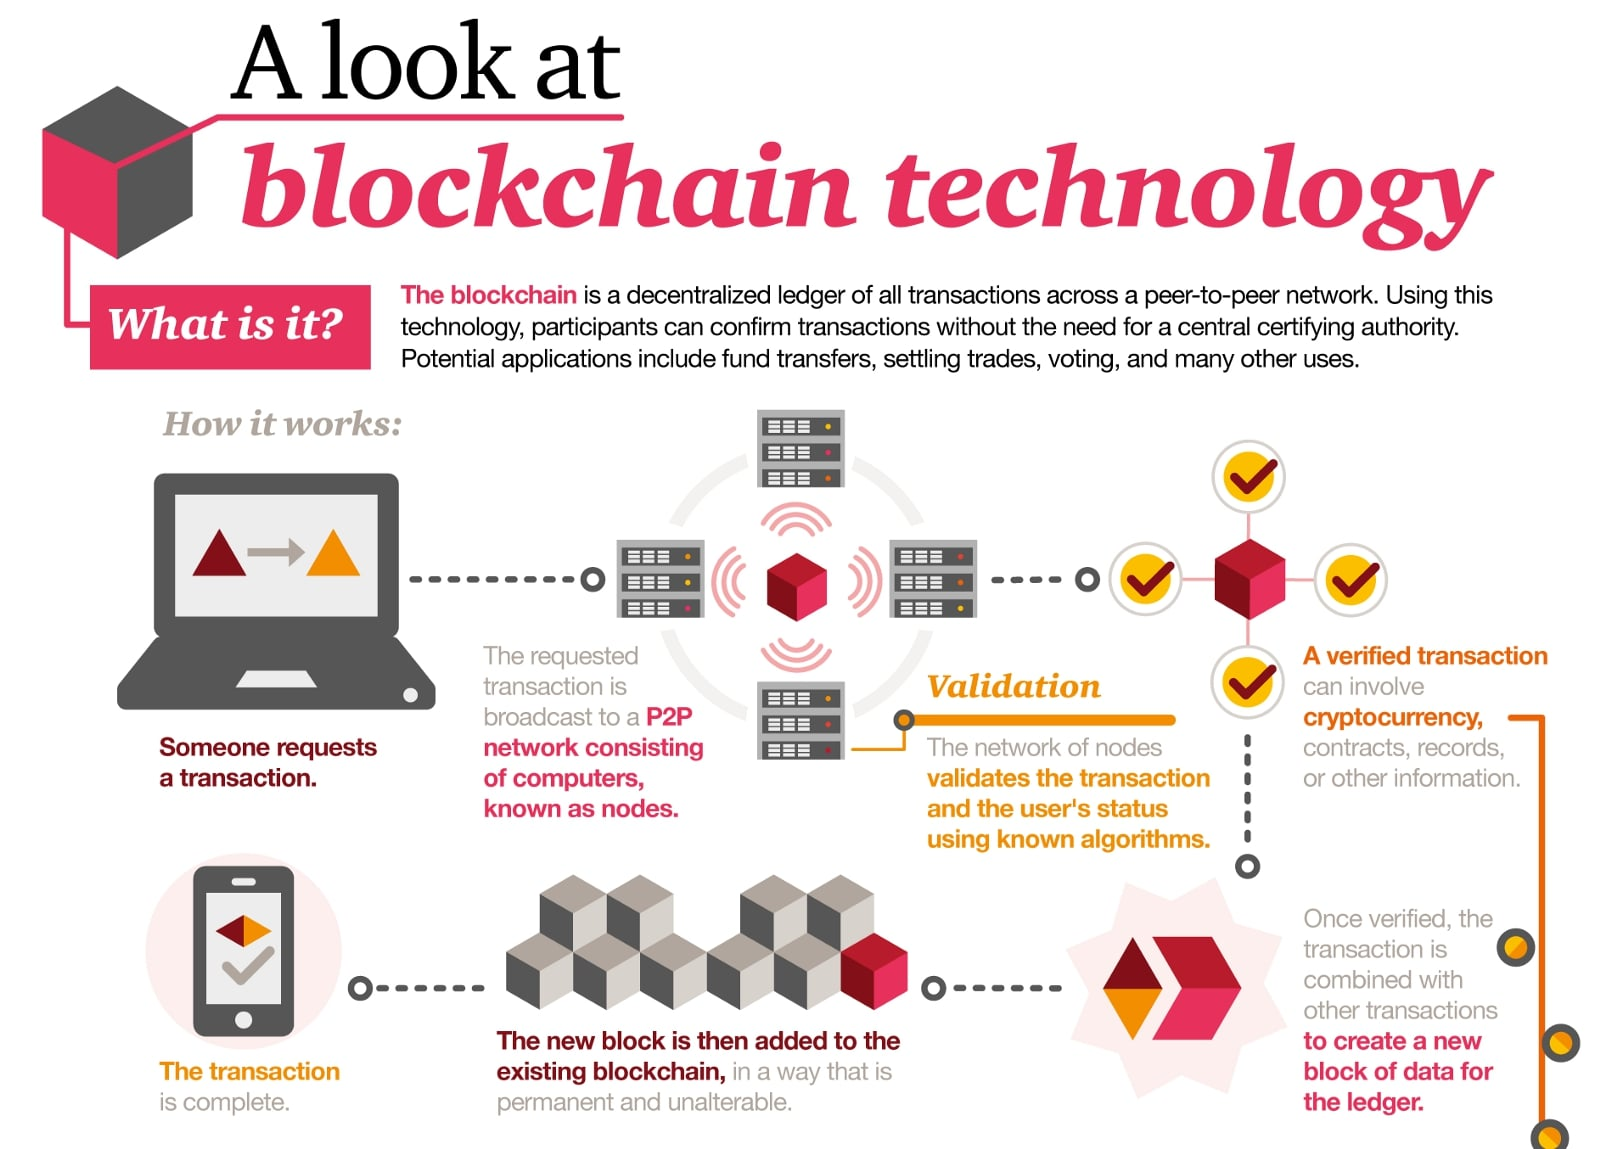
\includegraphics{blockchain.jpg}
		  \caption{Figure 5 : How Blockchain works}
\end{figure}

    \hypertarget{characteristics-of-a-blockchain}{%
\subsection{Characteristics of a
Blockchain}\label{characteristics-of-a-blockchain}}

    Understanding how a Blockchain works from a technical point of view is
valuable only to the extent of developing or troubleshooting one. In
order cohesively grasp the potential unto apply Blockchain technology,
you must also understand the characteristics of a Blockchain. It is
important to note that not all characteristics listed below will apply
to all Blockchains.

    \textbf{CONSENSUS}

Probably the most important characteristic of Blockchain is consensus.
Blockchain consensus refers to the ability of all anonymous network
participants agreeing network's rules are followed and there is only one
truth in the Blockchain environment. Consensus can be achieved in many
different ways such as Proof of Work (PoW) algorithm or Proof of Stake
(PoS) algorithm.

    \textbf{DISTRIBUTED COMPUTATION}

The impact capability of the Blockchain network is largely attributed to
its distributed architecture. Continuing with the Bitcoin Blockchain
example, each user that is running a full node on their computer will
have download a full copy of the whole Blockchain. Each full copy will
include data for all transactions recorded on the Bitcoin Blockchain.
After the copy has been downloaded the node can then run-independently
to process transactions and propagate them further across the network.
Nodes can also contribute to network-consensus via mining by including
transaction data in a block and then finding a proof-of-work for the
block. An important concept about Blockchain's distributed network is
that there is no central node processing and distributing the data, but
every node can run independently and broadcast any work that is proved.

    \textbf{INFORMATION STORAGE}

In the case of the Bitcoin Blockchain, information stored within the
blocks is btransactional data. However, this feature extends further
beyond just cryptocurrency transactions, and can extend into smart
contracts, as used on the Ethereum Blockchain.

    \textbf{PROVENANCE}

In traditional banking, you know your money is in the bank because the
bank tells you it is. In a Blockchain transaction, each activity is
tracked, recorded, and fully traceable without a third-party required to
attest to a specific action.

    \textbf{IMMUTABILITY}

No participant in the Blockchain network can modify a transaction after
it has been recorded. In case of error you cannot edit or undo it, the
erroneous record cannot be erased and is always be visible once
recorded. To correct the error a new transaction must be generated which
will reference the erroneous record.

    \textbf{ACCESS CONTROL}

In a shared open public ledger such as the Bitcoin Blockchain everyone
has access to view and append to the Blockchain. Conversely, a
Blockchain can be more privatized and have stricter access to who has
permissions to view and edit the Blockchain. These types of privatized
chains are typically found in private enterprise blockchains, where data
tends to be more sensitive.

    \hypertarget{types-of-blockchains}{%
\subsection{Types of Blockchains}\label{types-of-blockchains}}

    Blockchain is a continually evolving technology. Because of its
foundational technology characteristics, new applications are being
continuously developed on top of its framework. This means that new
there are new sets of requirements to support said innovations. These
new requirements mean a specific Blockchain that works for one
application, may not work for another. This problem is solved by
creating different types of Blockchains.

    We explore the three most common types of Blockchain below:

    \textbf{Public Blockchain}

Also called ``permissionless ledgers'', contain absolutely no
restrictions. Public Blockchains allow anyone to contribute data to the
ledger with all participants possessing an identical copy of the ledger.
Since there is no single owner of the ledger, this methodology is more
suitable for censorship resistant applications (e.g.~Bitcoin). Public
Blockchains often offer economic incentives for those who secure the
network.

    \textbf{Private Blockchain}

These networks are controlled by either a single or series of designated
network administrators. Private Blockchains allow for distributed
identical copies of a ledger, but only to a limited amount of trusted
participants only. As the network may have an owner(s), this methodology
is better suited for applications requiring simplicity, speed, and
greater transparency.

    \textbf{Hybrid Blockchain}

Also called ``consortium Blockchains'', are considered to be
semi-decentralized and employ characteristics of both public and private
blockchains. Hybrid Blockchains contain sets of permissions, similar to
private blockchains, however, instead of a single organization
controlling it, a group of agreed upon organizations control it.
Administers of each organization can restrict users' reading rights as
they desire and only allow a limited set of trusted nodes to execute a
consensus protocol.

    \hypertarget{bitcoin}{%
\subsection{Bitcoin}\label{bitcoin}}

    Bitcoin is a digital currency created in January 2009. It follows the
ideas set out in a white paper by the mysterious Satoshi Nakamoto, whose
true identity has yet to be verified. Bitcoin offers the promise of
lower transaction fees than traditional online payment mechanisms and is
operated by a decentralized authority unlike government-issued
currencies.

    The first exchange rate was 5 October 2009 and set the value of \$ 1 to
1309 BTC.

    Bitcoin first reached \$ 1,000 on November 27th, 2013.

    There are no physical Bitcoins, only balances kept on a public ledger in
the cloud that, along with all Bitcoin transactions, is verified by a
massive amount of computing power.

    Balances are kept using public and private ``keys'' which are long
strings of numbers and letters linked through the mathematical
encryption algorithm that was used to create them. The public key
(comparable to a bank account number) serves as the address which is
published to the world and to which others may send Bitcoins. The
private key (comparable to an ATM PIN) is meant to be a guarded secret
and only used to authorize Bitcoin transmissions.

    \hypertarget{how-bitcoin-works}{%
\subsection{How Bitcoin Works}\label{how-bitcoin-works}}

    Bitcoin is one of the first digital currencies to use peer-to-peer
technology to facilitate instant payments. The independent individuals
and companies who own the governing computing power and participate in
the Bitcoin network, also known as ``miners,'' are motivated by rewards
(the release of new Bitcoin) and transaction fees paid in Bitcoin. These
miners can be thought of as the decentralized authority enforcing the
credibility of the Bitcoin network. New Bitcoin is being released to the
miners at a fixed, but periodically declining rate, such that the total
supply of Bitcoins approaches 21 million. One Bitcoin is divisible to
eight decimal places (100 millionths of one Bitcoin) and this smallest
unit is referred to as a Satoshi. If necessary, and if the participating
miners accept the change, Bitcoin could eventually be made divisible to
even more decimal places.

    Bitcoin mining is the process through which Bitcoins are released to
come into circulation. Basically it involves solving a computationally
difficult puzzle to discover a new block which is added to the
blockchain and receiving a reward in the form of a few Bitcoins. The
block reward was 50 new Bitcoins in 2009 it decreases every four years.
As more and more Bitcoins are created, the difficulty of the mining
process -- that is, the amount of computing power involved -- increases.


\begin{figure}[H]
	\centering
		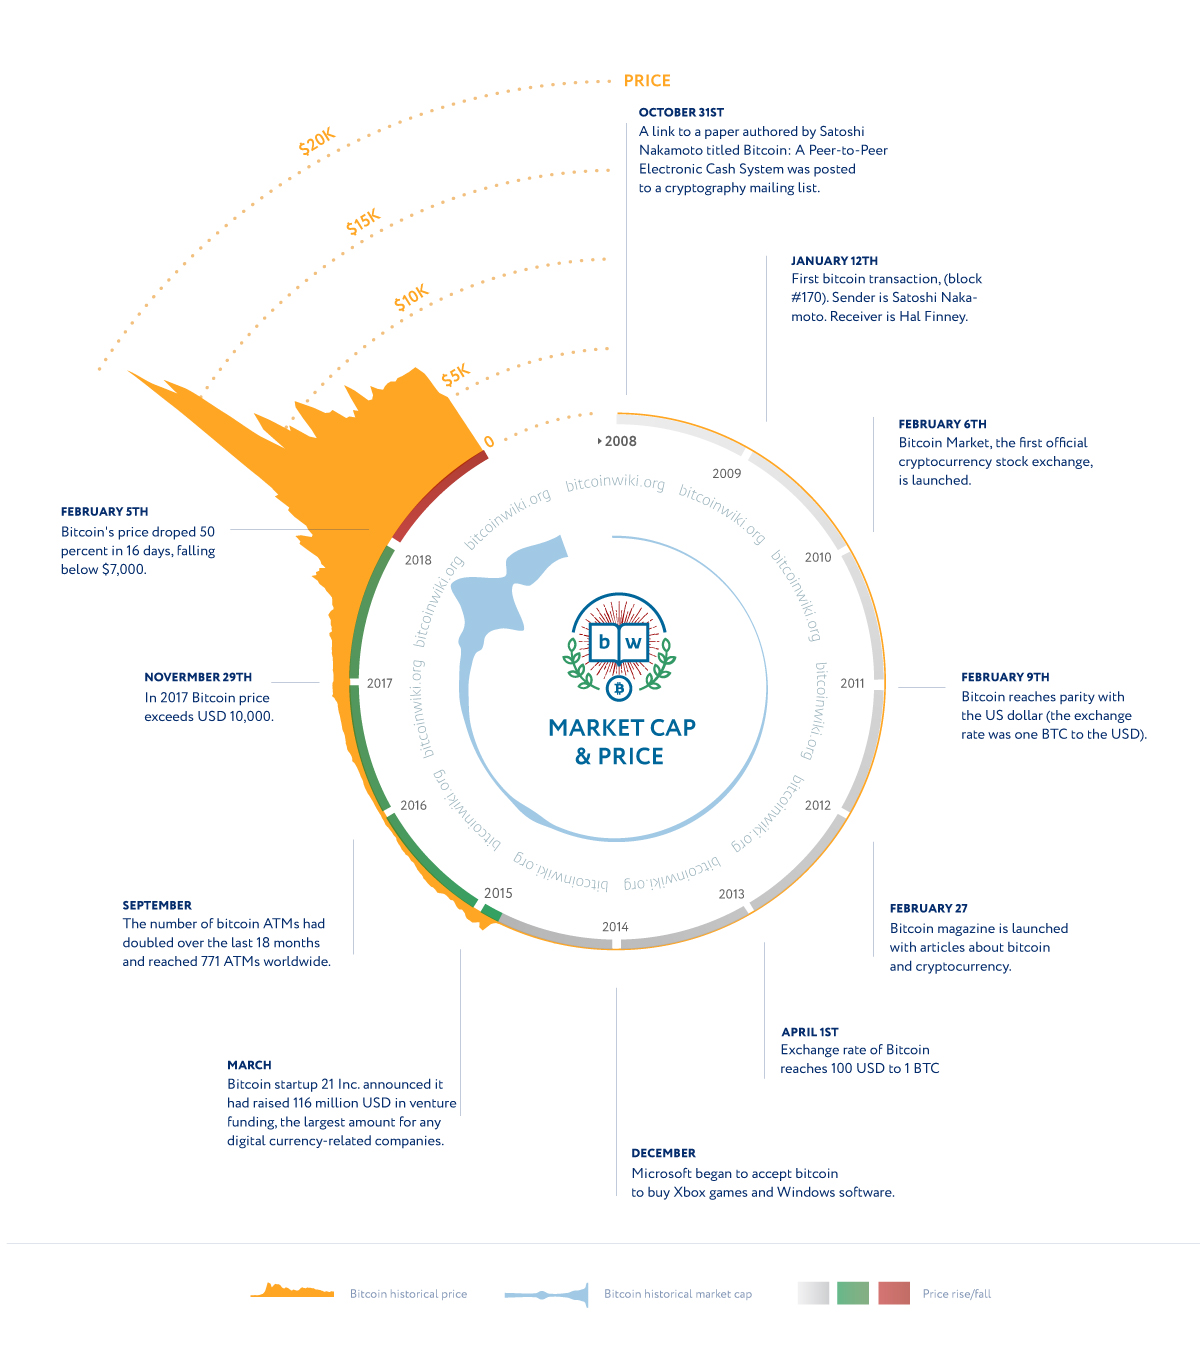
\includegraphics{history_price.jpg}
		  \caption{Figure 6 : History Price of Bitcoin}
\end{figure}

    \hypertarget{what-factors-affect-the-price-of-bitcoin}{%
\subsection{What factors affect the price of
Bitcoin?}\label{what-factors-affect-the-price-of-bitcoin}}

    There are several factors that can influence the price of Bitcoin more
or less profoundly:

    \textbf{Market demand and supply} - This is undoubtedly the most
important factor. To date, Bitcoin does not have a physical equivalent
in the real world, and can therefore only be sold using networked
Exchange services. One of the fundamental principles of the economy
explains that the more a currency is purchased the more its value
increases, and vice versa it is lowered when it is sold: the Bitcoin is
no exception, so much that in the last months of 2013 the price of the
currency multiplied by over ten times due to high demand from China.

    \textbf{Bitcoin and coin holders} - There are currently around 16
million Bitcoins in the world and, although new ones are being generated
every day, the maximum number of Bitcoins is around 21 million: since
the currency has a maximum unit cost, the price in the future is set to
increase.

    \textbf{News disclosed by the media} - The human factor should never be
underestimated, and how people react to news. We recall for example the
sharp reduction in the price following the arrest of Ross Ulbricht or
the record figures reached shortly before the decision of the SEC on
ETFs.

    \textbf{Technical problems} - The code behind Bitcoin is totally open
source, and can therefore be examined by anyone. Updates aimed at fixing
bugs or strengthening some weak areas of the code can drive up prices.
Conversely, account hacking or DDoS attacks on major companies can make
it crash.

    \textbf{World political and economic events} - In a globalized world
like ours, the decisions of a single country can affect the entire
planet: it was the case of Japan which began accepting payments starting
from the first half of 2017 in Bitcoin.

    \textbf{Strong instability} - In the world of finance, the term
``volatility'' means the degree of change in prices over a certain
limited period of time. The value of a highly volatile security may
increase or decrease from one moment to another, moving along a very
wide price scale: the result of the investment is therefore uncertain
and potentially risky.


    % Add a bibliography block to the postdoc
    
    
    
    \end{document}
